\documentclass[12pt]{report}

% This first part of the file is called the PREAMBLE. It includes
% customizations and command definitions. The preamble is everything
% between \documentclass and \begin{document}.

\usepackage[margin=1in]{geometry}  % set the margins to 1in on all sides
\usepackage{graphicx}              % to include figures
\usepackage{amsmath}               % great math stuff
\usepackage{amsfonts}              % for blackboard bold, etc
\usepackage{amsthm}                % better theorem environments
\usepackage{import}
%\documentclass{report}
\usepackage{url}
\usepackage{natbib}
\usepackage{chapterbib}

% Packages for pyFRET chapter
\usepackage{amsmath}
% amssymb package, useful for mathematical symbols
\usepackage{amssymb}

% graphicx package, useful for including eps and pdf graphics
% include graphics with the command \includegraphics
\usepackage{graphicx}

% cite package, to clean up citations in the main text. Do not remove.
%\usepackage{cite}
\usepackage{hyperref}
\usepackage{color} 

\usepackage{listings}

% Packages for Illumina chapter
\usepackage{multirow}
\usepackage{hyperref}
\usepackage{parskip}
\usepackage{subfigure}


\definecolor{dkgreen}{rgb}{0,0.6,0}
\definecolor{gray}{rgb}{0.5,0.5,0.5}
\definecolor{mauve}{rgb}{0.58,0,0.82}

\lstset{frame=tb,
  language=Python,
  aboveskip=3mm,
  belowskip=3mm,
  showstringspaces=false,
  columns=flexible,
  basicstyle={\small\ttfamily},
  numbers=none,
  numberstyle=\tiny\color{gray},
  keywordstyle=\color{blue},
  commentstyle=\color{dkgreen},
  stringstyle=\color{mauve},
  breaklines=true,
  breakatwhitespace=true,
  tabsize=3
}



\begin{document}


\title{Thesis of DOOM}

\author{Rebecca Roisin Murphy \\ 
Department of Chemistry \\
University of Cambridge \\
Lensfield Road, Cambridge, CB2 1EW}

\maketitle

\begin{abstract}
  My PhD thesis.
\end{abstract}

\tableofcontents

\chapter*{Acknowledgements}
\emph{Had I the heavens' embroidered cloths,\\
	Enwrought with golden and silver light,\\
	The blue and the dim and the dark cloths\\
	Of night and light and the half-light,\\
	I would spread the cloths under your feet:\\
	But I being poor have only my dreams;\\
	I have spread my dreams under your feet;\\
	Tread softly because you tread on my dreams.\\
	\bf{W. B. Yeates}\\
}

This thesis presents more than three years of work at the University of Cambridge, during which time I have had the privilege to meet and work with many fantastic people. Please allow me to begin by thanking those of you who have supported and encouraged me in my research work -- without you, nothing that I achieved would have been possible.

First and foremost, I would like to thank my supervisors, David Klenerman and Sophie Jackson. Thank you both for your continued support and encouragement, despite the somewhat unusual structure and focus of my PhD. Thank you for giving me the freedom to pursue my research interests and for allowing me to find a path that is my own, if somewhat unconventional.

To my colleagues in the Klenerman and Jackson groups, thank you all for making my time in the Chemistry Department so enjoyable. Particular thanks are due to:

\begin{itemize}
\item[] Mathew, for many many invaluable conversations about data, sizing and thresholding. Your enthusiasm for research, your attention to detail and your ability to get things done are all phenomenal. I wish you great success and great happiness in your future research career. Enjoy your life as an expatriate.
\item[] Vladas, you were a fantastic collaborator and Masters student throughout your research project, even though it was somewhat ``wetter'' than you might have hoped. The Holliday Junctions that you prepared have been invaluable to our research on oligomer sizing and have given the group many useful insights. Thank you also for sharing Marmalade!
\item[] Alex, for your amazing skills with hardware description languages and all of your custom FPGA correlators. Without your expertise, none of this research could have been done. Thank you also for your patience in the face of my lack of physics knowledge and your assisstance with signal generators.
\item[] Kristina, for your help with TIRF experiments, as well as for many interesting discussions about data analysis and statistics. As a scientist, you are an inspiration.
\item[] Magnus, for all your support with pyFRET, in particular your enthusiasm to test new functionality and all your suggestions for improvements. Your encouragement took this from just an idea to something real and made me a much better sofware engineer in the process.
\item[] Yu, thank you for many interesting discussions about data, your honesty, and your eventual agreement that actually I am quite clumsy in the lab!
\item[] Steve, thank you for many helpful discussions. Your enthusiasm and insight have dramatically improved my understanding of optics, light and physics generally. Your guidance and collaboration helped to bring many ideas from theoretical concept to concrete reality.
\end{itemize}

Gratitude is also owing to the Algorithms Group at Illumina, who made my internship there such an interesting and memorable experience. In particular, I would like to thank Ole and Jared for all their patience and understanding, as well as for your support in bringing such an interesting project to reality.

To George, my partner. Thank you for your unconditional support, your infinite love and the best conversation in the world. Thank you for introducing me to the magic that is programming and for your many hours debugging my early spaghetti attempts at writing code. You have brought more to my life than you can imagine.

To James, my colleague and friend, thanks are owing for many years of great discussions, tea and cynicism. Thanks for your support and for telling me to get my act together.

Finally to my family: Granny, Mum and Peter, thank you all so much for your help and support throughout my life. Thank you for teaching me about the truly important things: kindess, integrity and honesty. And Grandad, thank you for your early enouragement on my scientific journey. Thank you for teaching me about evidence and proof. I hope you would be proud of me today. 
\chapter*{Summary}
%\section{General Introduction}
%\section{Contributions}
%\section{Thesis Overview}
Single molecule fluorescence microscopy describes a number of experimental techniques for the study of individual molecules using fluorescence detection. Single molecule microscopy has found a wide range of research applications. These applications include the study of protein folding, protein aggregation and intermolecular associations. Since the first demonstration of the detection of a single, fluorescently-labelled molecule, considerable effort has been made to improve the quality of the data obtained, through the development of novel experimental methodologies.

However, the development of novel experimental methods requires the concommitant development and rigorous evaluation of analysis tools that can maximise the information available from the data obtained. This thesis describes the development and thorough evaluation of data analsysis methodologies for confocal single molecule fluorescence microscopy. We describe the implementation of an open source software library for the analysis of confocal single molecule fluorescence data, and the systematic evaluation of existing data analysis methodologies. We then describe the development of a novel method of data analsysis, based on Monte Carlo sampling. We apply this analysis methodology to the calculation of intramolecular distances and to the determination of oligomer sizes using confocal fluorescence microscopy. We then describe a thorough evaluation of the performance of these analysis methods. A final chapter describes the development of an error correction tool for genome assemblies generated using fluorescence-based sequencing technology from Illumina.

Overall, the work described in this thesis describes the development and systematic evaluation of computational techniques for the analysis of fluorescence data. We describe the theoretical basis of novel techniques and the deployment and analysis of both novel and existing methodologies. In completing this work, we hope to provide a stable foundation on which further research can be built, both through application of the techniques described here and through their extension to further experimental techniques.

%To date, the same attention has not been paid to data analysis. Analysis of single molecule fluorescence data is typically considered of secondary importance to data collection. As a consequece of this, the development and evaluation of data analysis tools for single molecule fluorescence microscopy have lagged behind development of experimental techniques. 



%The rest of this thesis is structured as follows. Chapter 2 provides a introduction to other research that has been undertaken in the field of fluorescence microscopy. General experimental and analysis techniques for fluorescence microscopy of single molecules are introduced, and the work presented in this thesis is contextualised. Chapter 2 also provides an overview of current research in Bayesian statistics and probabilistic analysis, introducing the statistical methods that are used in later chapters. Following this introductory section, we present our results over four separate chapters.

%Chapter 3 introduces the pyFRET library, which we developed for analysis of confocal smFRET data. We describe the theory and implementation of different analysis algorithms for smFRET datasets. Data from both continuous and alternating excitation experiments are considered. In the second part of Chapter 3, we provide a comprehensive evaluation of different smFRET analysis algorithms, using a combination of simulated and experimental datasets. We benchmark popular analysis techniques, demonstrating their relative utility under different data collection regimes.

%Chapter 4 considers a Bayesian method for the analysis of data from continuous excitation smFRET datasets. First, we introduce a model-based theory of the smFRET experiment. Then, we describe how this parametric model can be used to infer intramolecular distances and population sizes from time-binned smFRET data. We benchmark our Bayesian analysis technique against thresholding techniques used for time-binned data, showing the superior performance of the inference technique.

%Chapter 5 extends this Bayesian analysis to sizing of labelled protein aggregates. We describe how a simplified model can be used to describe photon emission from multiple fluorophores. Using a combination of real and simulated datasets, we then show that this model is degenerate, making inference of aggregate sizes undecidable. We further show that a single emission event has multiple sources of heterogeneity, creating a complex, non-linear relationship between aggregate size and the number of photons emitted in a fluorescent event.

%Chapter 6, the final results chapter, is somewhat different. This chapter describes a Bayesian analysis tool for error correction in genome assemblies generated using Illumina Nextera mate pairs. Illumina sequencing technology uses fluorescence emission from multiple fluorophores in its base calling algorithm. However, base calling errors and complex repeat structures can make reassembly of short reads challenging. In this chapter, we introduce NxRepair, an error correction tool that can identify mistakes in {\emph de novo} assemblies of bacterial genomes. We benchmark NxRepair against existing tools, demonstrating its superior performance.

%Finally, Chapter 7 provides the conclusion to the thesis. Here, we summarise the overall contribution of this thesis and relate the work described to its wider research context. We also discuss possible extensions of the research described, indicating future applications of the research.
\chapter{Introduction}
\label{chap:intro}
\section{Introduction}
This chapter provides a general introduction to the contextual background of the work presented in this thesis. First, we provide a general overview of the physical phenomena of fluorescence and F\"{o}rster resonance energy transfer (FRET) and describe how these pheonomena can be applied to the study of biological molecules. We also review the common experimental and analytical techniques used in these research areas. We then present an overview of techniques of statistical analysis, with a particular focus on model-based Bayesain inference. We present common sampling-based techniques for Bayesian statistical analysis and describe why Bayesian inference is a useful tool in the analysis of single-molecule fluorescence data.

\section{Fluorescence and FRET}
Since FRET was first used to measure the distance between two fluorescent dyes on individual molecules bound to a surface~\cite{ha96}, single-molecule FRET (smFRET) has become a popular tool to investigate the structure and dynamics of biomolecules, both on a surface and diffusing freely in solution~\cite{haran03, schuler02, weiss00}. We open this chapter with a discussion of the physical basis of molecular fluorescence and FRET. We then describe some of the applications of fluorescence in biological research, and describe the constraints and experimental techniques commonly used in single molecule fluorescence microscopy.

\subsection{The Physical Basis of Fluorescence}
\paragraph{Fluorescence}
Fluorescence is the physical phenomenon by which a molecule that has absorbed a photon of electromagnetic radiation and which is in an excited state relaxes via non-radiative processes, such as vibrational interactions, rotation and translation in its medium and then  emits a photon, returning to its ground state~\cite{valeur2001}. Typically, a fluorescence excitation-emission cycle involves transitions between the singlet ground state ($\text{S}_0$) and first excited state ($\text{S}_1$) of the fluorophore (Fig.~\ref{fig:jablonski}). Owing to the intramolecular transitions occurring prior to emission, the photon emitted is of a lower energy than the photon absorbed. The difference in energy between the absorbed and emitted photons is termed the Stokes shift (Fig.~\ref{fig:stokes},~\cite{Albani2011}) and is a characteristic of the energy levels available to the excited molecule. 

The typical timescale for a single fluorescence excitation-emission cycle is approximately $10^{-10} - 10^{-7}$ s. This timescale is dominated by the lifetime of the excited state, (typically $10^{-10} - 10^{-7}$ s); photon excitation and emission processes, as well as vibrational transitions, occur on a timescale that is several orders of magniude shorter (absorption $10^{-15}$ s, relaxation $10^{-12} - 10^{-10}$ s).

\begin{figure}[!ht]
   \begin{center}
      \includegraphics*[clip=true, width=6in]{introduction/jablonski.pdf}
      \caption{Schematic Jablonski diagram depicting the possible electronic processes undergone by an excited fluorophore. Solid lines indicate electronic transitions, wavy lines indicate vibrational transitions. Absorption of a high-energy photon promotes an electron from the ground state $\text{S}_0$ to an excited state, typically $\text{S}_1$. Fluorescence emission occurs during the electronic relaxation from $\text{S}_1$ to $\text{S}_0$. Non-radiative relaxation via internal conversion (IC) or other competing processes, such as inter-system crossing (ISC) to the triplet state $\text{T}_1$, reduce the quantum yield. Figure adapted from~\cite{Horrocks2014}, with permission.}
      \label{fig:jablonski}
   \end{center}
\end{figure}

\begin{figure}
	\begin{center}
	\includegraphics*[clip=true, width=3in]{introduction/QuantaRed-Spectra.jpg}
	\caption{The absorption (black line) and emission (red line) spectra for the Quanta Red dye. Due to fast vibrational relaxation, the fluorescence emission is shifter to longer wavelengths than the absorption. This is termed the Stokes shift. Figure from~\cite{spectral}}
	\label{fig:stokes}
	\end{center}
\end{figure}

\paragraph{Competing Processes}
In addition to the $\text{S}_1$ to $\text{S}_0$ transition that results in fluorescence emission, other competing energetic transitions can also occur, resulting in non-radiative relaxation to the ground state $\text{S}_0$, or permanent changes to the electronic structure of the fluorophore (photobleaching). Internal conversion -- a non-radiative transition to a lower energy state of the same spin multiplicity -- is possible, although the large energy gap between the $\text{S}_1$ and $\text{S}_0$ states makes it much less frequent than the more accessible fluorescent pathway. A more significant competitor is inter-system crossing, involving a non-radiative transition from the first singlet excited state, $\text{S}_1$ to the first triplet excited state, $\text{T}_1$. Although forbidden by spin selection rules, inter-system crossing is facilitated by spin-orbit coupling, allowing it to compete with fluorescence (rate $10^{-10} - 10^{-8}$ s) as a relaxation pathway.

From the $\text{T}_1$ state there are several accessible pathways to the ground state ($\text{S}_0$). Phosphorescence is the radiative decay from $\text{T}_1$ to $\text{T}_0$; alternatively, a second inter-system crossing back to $\text{S}_1$, followed by delayed fluorescence emission to reach the $\text{S}_0$ state is more common. As the lifetime of the $\text{T}_1$ state is long (on the order of $10^{-6} - 1$ s), this can be observed as photoblinking. These two processes are illustrated in Fig.~\ref{fig:jablonski}.  

A third relaxation pathway from the $\text{T}_1$ state is photobleaching. If the fluorophore is in a solution containing dissolved oxygen, the $\text{T}_1$ state can interact with the triplet ground state of molecular oxygen, leading to de-excitation via triplet-triplet annihilation:

\begin{equation}
^3\text{T}_1 + ^3\text{O}_2 \longrightarrow ^1\text{S}_0 + ^3\text{O}_2
\label{eq:blinking1}
\end{equation} 

The resultant singlet oxygen can then irreversibly oxidise the fluorophore, leaving it unable to undergo further fluorescent excitation-emission cycles.   

%Intersystem crossing ($10^{-10} - 10^{-8}$ s) and internal conversion ($10^{-11} - 10^{-9}$ s) are slower processes.

\paragraph{The Extinction Coefficient and Quantum Yield}
\label{par:qy}
In choosing a fluorophore for a single molecule fluorescence experiment, it is desirable to maximise the number of successful absorption-emisssion cycles undergone per unit time. Hence, the best fluorophores both absorb many exciting photons, increasing the number of possible cycles, and return to the ground state via fluorescence emission following the majority of excitations, maximising the number of photons actually emitted. Two key parameters that enable quantitative evaluation of fluorescent properties are the molar extinction coefficient, $\epsilon$, and quantum yield, $\phi$. 

The extinction coefficient, $\epsilon$, measures how strongly a fluorophore absorbs light at a given wavelength $\lambda$. It can be calculated for a fluorophore $f$, from the Beer-Lambert law~\cite{goldbook2006} as:

\begin{equation}
I = I_0 e^{-\epsilon_f l}
\label{eq:ext_coeff}
\end{equation}

where for an initial excitation intensity $I_0$, $I$ is the excitation intensity at a distance $l$ into a solution of fluorophore $f$ and $\epsilon_f$ is the extinction coefficient of the fluorophore.

Similarly, the fluorescence quantum yield for fluorophore $f$, $\phi_f$, describes the fraction of photon absorption events that result in emission of a photon. It can be defined as: 

\begin{equation}
\phi_f = \frac{k_f}{k_f + k_{nr}}
\label{eq:quantum_yield}
\end{equation}

where $k_f$ and $k_{nr}$ are the rates of fluorescence emission and non-radiative emission respectively. When all molecules in the excited state were promoted by photon absorption, $\phi_f$ can be equivalently defined as the fraction of absorption events that result in fluorescence emission: 


\begin{equation}
\phi_f = \frac{n_{\text{emitted}}}{n_{\text{absorbed}}}
\label{eq:quantum_yield_ratio}
\end{equation}

where $n_{\text{emitted}}$ and $n_{\text{absorbed}}$ are respectively the number of emitted and absorbed photons.

%The energetic interconversions involved in fluorescence can be summarised using a Jablonski diagram (Fig.~\ref{fig:jablonski}).

\subsection{The Physical Basis of FRET}
\label{sect:fret}
\paragraph{F\"{o}rster Resonance Energy Transfer}
F\"{o}rster resonance energy transfer (FRET) is a non-radiative energy transfer process that can occur between chromophoric molecules~\cite{forster48}. The degree of energy transfer, E, is dependent on the fluorophore distance, varying inversely with the sixth power of the dye-dye distance, $r$: 

\begin{equation}
E = \frac{1}{1+ (\frac{r}{R_0})^6}
\label{eq:FRET_d}
\end{equation}

where, $R_0$ is the F\"{o}rster distance, a dye-dependent constant that defines the dye-dye distance for which the energetic transfer efficiency is 50 \%. $R_0$ is defined, for a donor (D) and acceptor (A) fluorophore pair, by their degree of spectral overlap and their relative orientation:

\begin{equation}
R_0 = \sqrt[\leftroot{-2}\uproot{2}6]{\frac{9000\phi_D\ln(10)\kappa^2J(\lambda)}{128\pi^2n^4N_A}}
\label{eq:R_0}
\end{equation}

Here, $\phi_D$ is the quantum yield of the donor fluorophore, $\kappa$ is the dipole orientation factor, $N_A$ is Avogadro's number, n is the refractive index of the medium, and $J(\lambda)$ is the spectral overlap integral:

\begin{equation}
J(\lambda) = \int f_D(\lambda)\epsilon_A(\lambda)\lambda^4\,d\lambda
\label{eq:J}
\end{equation}

where $f_D(\lambda)$ and $\epsilon_A(\lambda)$ are respectively the normalised emission spectrum of the donor and the molar extinction coefficient of the acceptor at wavelength $\lambda$. The dipole orientation factor, $\kappa^2$ is typically assumed to be $\frac{2}{3}$, the value observed if both dyes are freely rotating and hence can be assumed to be isotropically oriented during the lifetime of the $\text{S}_1$ excited state~\cite{Demchenko2008}.

\paragraph{Deriving the FRET Equation}
The distance dependence of the energy transfer allows FRET to be used as a ``molecular ruler"~\cite{stryer67}, to determine intramolecular distances. For a given FRET enrgy transfer event, the FRET Efficiency, $E$, defined with respect to the intramolecular distance $r$ in Eq.~\ref{eq:FRET_d}, is given ratiometrically by:

\begin{equation}
E = \frac{n_A}{\gamma \cdot n_D + n_A}
\label{eq:FRET_E}
\end{equation}

where $n_A$ and $n_D$ are the number of observed photons emitted by the acceptor and donor fluorophores respectively, and $\gamma$ is an instrument-dependent constant that corrects for unequal detection efficiencies. The equivalence of Eq.~\ref{eq:FRET_d} and Eq.~\ref{eq:FRET_E} is derived below.

As defined above, the quantum yield of a (donor) fluorophore is given by the ratio of the rates of decay from the excited state $\text{S}_1$ via radiative and non-radiative processes: 

\begin{equation}
\phi_D = \frac{k_f}{k_f + k_{nr}}
\label{eq:quantum_yield_donor}
\end{equation}

Similar ratios can be used to describe the quantum yield of a donor fluorophore that can undergo FRET energy transfer (Eq.~\ref{eq:quantum_yield_donor_FRET}) and the FRET efficiency (Eq.~\ref{eq:FRET_ratio}):

\begin{equation}
\phi_{DA} = \frac{k_f}{k_f + k_{nr} + k_{ET}}
\label{eq:quantum_yield_donor_FRET}
\end{equation}

\begin{equation}
E = \frac{k_{ET}}{k_f + k_{nr} + k_{ET}}
\label{eq:FRET_ratio}
\end{equation}

where $k_{ET}$, the rate constant for the FRET energy transfer process, is given by:

\begin{equation}
k_{ET} = \frac{1}{t_D} \left(\frac{R_0}{r}\right)^6
\label{eq:k_ET}
\end{equation}

and $t_D$ is the lifetime of the excited state in the absence of an acceptor fluorophore: 

\begin{equation}
t_D = \frac{1}{k_{f} + k_{nr}}
\label{eq:ex_lifetime}
\end{equation}

Combining Equations~\ref{eq:quantum_yield_donor},~\ref{eq:quantum_yield_donor_FRET} and~\ref{eq:FRET_ratio} yields:

\begin{equation}
\begin{split}
E &= 1 - \frac{k_{f} + k_{nr}}{k_f + k_{nr} + k_{ET}} \\ 
&= 1 - \frac{\phi_{DA}}{\phi_{D}} \\
&= 1 - \frac{n_{DA}}{n_{D}}
\label{eq:FRET_ratio_2}
\end{split}
\end{equation}

where $n_{DA}$ and $n_D$ are respectively the number of observed photons emitted by the donor fluorophore in the presence and absence of a FRET acceptor at distance $r$.

In the presence of a FRET acceptor, it is not possible to directly observe $n_D$. However, this can be derived from the number of photons observed to be emitted by the acceptor fluorophore, $n_A$. The difference in the number of photons emitted by the donor in the presence and absence of the acceptor is $n_D - n_{DA}$. This is related to the number of photons emitted by the acceptor, $n_A$, as follows:

\begin{equation}
\frac{n_D - n_{DA}}{n_A} = \frac{\phi_D\eta_D}{\phi_A\eta_A}
\label{eq:ratio_FRET}
\end{equation}

where $\phi_D$ and $\phi_A$ are the quantum yields of the donor and acceptor fluorophores respectively, and $\eta_D$ and $\eta_A$ are the respective instrumental detection efficiencies of donor and acceptor photons.

If we call the ratio $\frac{\phi_D\eta_D}{\phi_A\eta_A}$ $\gamma$, Eq.~\ref{eq:ratio_FRET} can be re-arranged to give:

\begin{equation}
n_D = n_{DA} - \frac{n_A}{\gamma}
\label{eq:get_gamma}
\end{equation}

Substituting this definition of $n_D$ back into Eq.~\ref{eq:FRET_ratio_2} yields the expected definition of E,~\ref{eq:FRET_E}, that allows the inter-fluorophore distance to be related to an experimentally observed ratio of donor and acceptor photons.

%\section{Fluorescence Microscopy}
\section{Single Molecule Fluorescence Microscopy}
Both fluorescence and FRET have found many applications in the study of biological systems. Fluorescence microscopy is a well-established field of research, which uses fluorescence emission to generate an image. Synthetic or naturally occurring fluorophores are conjugated to biomolecules of interest and then excited using monochromcatic light matched to the fluorophore's absorption spectrum~\cite{Michalet2003}. Photons emitted from the fluorophores are collected and used to gain information about the structures and associations of the labelled molecules. 

Advances in the fields of optical microscopy, fluorophore synthesis and data analysis have facilitated development of optical techniques that are sensitive enough to detect emission from individual fluorophores. This has created the field of single molecule fluorescence microscopy and the capacity to characterise the behaviour of individual biomolecules. The following section describes the benefits of single molecule fluorescence microscopy, introduces the main optical systems used for single molecule imgaing, and discusses the experimental and analytical challenges involved in a single molecule experiment. As the main experimental technique used in this thesis, we focus our discussion on single molecule confocal spectroscopy; however, for context, we include an overview of other single molecule fluorescent techniques.  

%Fluorescence can be used simply to gain information about cellular organisation and molecular localisations; for example by fluorescently labelling specific cellular structures with organic dyes and then imaging planes of the entire cell to identify  
\subsection{Techniques of Single Molecule Imaging}
The greatest challenge in single molecule microscopy is to be able to detect dim fluorescence emission from individual molecules against a background of photon emission from other sources, such as Raman scattering by solution molecules and residual fluorescence from solution impurities~\cite{Moerner2003}. Consequently, a large amount of work has been done to maximise the signal-to-noise ratio (SNR) of fluorescent emission data. This ratio can be optimised from both ends; namely maximising the signal and minimising the background noise. Maximising the signal involves the development and selection of fluorophores that achieve many fluorescent emission cycles during an excitation event. This is discussed in Section~\ref{sect:fluorophores}. 

An effective way to minimize the background noise is to reduce the emission detection volume; as the number of photons detected from irrelevant species will be reduced with a smaller detection volume, whereas detection of photons from a single fluorophore of interest within the detection volume will be unaffected~\cite{Dillingham2008}. Single molecule fluorescence techniques can hence be characterised based on their method of detection volume reduction: Wide-field techniques, including Epifluorescence Microscopy and Total Internal Fluorescence Microscopy (TIRFM) illuminate and collect data from a wide image plane with a large area but minimal depth; by contrast confocal microscopy techniques attempt to collect data from the smallest detection volume possible -- a voxel of volume approximately 1 fL. These techniques and the optical geometry required for successful data collection, are summarized below. 

\paragraph{Epifluorescence Microscopy}
The simplest geometry for single molecule fluorescence detection is epifluorescence microscopy (Fig.~\ref{fig:epi}). In an epifluorescence microscope monochromatic, collimated light is focused into the back apperture of an objective lens with a high Numerical Aperture (N.A.). A large volume of the fluorescently labelled sample, which is placed above the objective, is illuminated; emitted photons are collected through the same objective. Fluorescence emission is separated from excitation light using various filters before being focused onto a charge coupled device (CCD) camera which generates a current at each pixel proportional to the intensity of incident light.

\begin{figure}
	\begin{center}
	\includegraphics*[clip=true, width=2in]{introduction/epi.pdf}
	\caption{Schematic of an epifluorescence microscope. Laser light is focused into a sample using an objective lens with a high N.A. Emitted fluorescence is captured using the same objective, separated from reflected exciting photons using a dichroic mirror and directed onto a CCD.}
	\label{fig:epi}
	\end{center}
\end{figure}

The principal advantage of epifluorescent illumination, in addition to its ease of set-up, is the large illumination area. The detection volume is typically seveal microns in diameter, allowing multiple emitters to be imaged at the same time and to be tracked across multiple image frames~\cite{Webb2014}. However, because the depth of the illumination volume in epifluorescence microscopy is relatively large, the SNR is quite low: many molecules at different depths into the sample volume are illuminated, resulting in a large amount of out-of-focus fluorescence reaching the CCD camera. Consequently, although epifluorescence microscopes are the most commonly used variant of the fluorescence microscope, they are less useful for single molecule detection, as the SNR is too low to efficiently resolve fluorescence emission from individual molecules.

\paragraph{Total Internal Fluorescence Microscopy}
Total Internal Fluorescence Microscopy (TIRFM) (Fig.~\ref{fig:TIRF} A) uses a similar optical geometry to epifluorescence microscopy: as in epifluorescence imaging, the sample is illuminated via the back port of an objective and fluorescence emission is collected via the same objective and focused onto a CCD camera. Howerver, TIRFM exploits the phenomenon of Total Internal Reflection (TIR) to reduce the depth of the illumination volume and hence increase the SNR.

\begin{figure}
	\begin{center}
	\includegraphics*[clip=true, width=6in]{introduction/tirf.pdf}
	\caption{A) Schematic of a TIRF microscope. As in epifluorescence, laser light is focused into a sample using an objective lens with a high N.A. Emitted fluorescence is captured using the same objective, separated from reflected exciting photons using a dichroic mirror and directed onto a CCD. However, because the excitation wavelength meets the glass coverslip at an angle exceeding the critical angle, only molecules very close to the coverslip are excited. B) For two materials with refractive indices $n_2 < n_1$, TIR occurs when the incident angle, $\theta$, exceeds the critical angle $\theta_c$.}
	\label{fig:TIRF}
	\end{center}
\end{figure}

TIR occurs when a light wave passing through a medium with refractive index $n_1$ meets a dielectric medium with refractive index $n_2 < n_1$ with an incident angle $\theta$, where $\theta > \theta_c$, the critical angle (Fig.~\ref{fig:TIRF} B). Under these conditions, rather than some of the light being refracted at the boundary between the two media, all of the light is reflected internally. As a result of the TIR, an evanescent wave is generated at the boundary. This wave is propagated along the boundary, but decays exponentially with distance from the boundary. The distance that the wave penetrates beyond the boundary is dependent on the incident angle $\theta$, decreasing as $\theta$ increases. 

The critical angle, $\theta_c$ is determined using Snell's Law~\cite{Wolf1995} using the ratio of the refractive indices $n_1$ and $n_2$:

\begin{equation}
\theta_c = \sin^{-1}\left(\frac{n_2}{n_1}\right)
\label{eq:snell}
\end{equation}

For a typical borosilicate coverslide ($n = 1.518$) in contact with water ($n = 1.33$), a TIRF angle of $61.2^{\circ}$ is required, enabling fluorescence excitation to be limited to a depth of $\sim 100$ nm. The narrow excitation depth of TIRFM allows all of the advantages of epifluorescence (specifically large excitation area and particle tracking), but increases the SNR sufficiently that fluorescence emission from individual molecules can be effectively resolved.

%\paragraph{Super-Resolution Microscopy}
\paragraph{Confocal Microscopy}
Confocal microscopy takes the reduction in excitation volume a further step, minimizing the detection volume in all dimensions and collecting fluorescence emission from a solution volume of $\sim 1$ fL. In confocal microscopy (Fig.~\ref{fig:confocal}), a collimated laser beam is focused through an infinity corrected objective with a high N.A. onto a diffraction limited spot (diameter $> 1 \mu$m) a few microns into the sample volume. Fluorescence emission from the sample is collected and recollimated by the same objective, passed through a dichroic mirror to remove reflected incident light and then directed through a small aperture pinhole (diameter $50 - 100 \mu$m) placed in the conjugate focal plane to remove out-of-focus fluorescence. The remaining photons are directed onto an Avalanche Photodiode (APD) detector, which can detect individual photons with nanosecond resolution. To enable detection of fluorescence from individual fluorescent molecules, analyte solutions are used at extremely low concentrations (typically $10 - 100$ pM), such that the probability of more than one molecule occupying the confocal volume simultaneously is extremely small. Single molecule confocal microscopy is typically used in this manner to image labelled molecules diffusing freely in solution~\cite{weiss00} or flowed rapidly through the exciting laser beam~\cite{horrocks2012}; in conjunction with a moveable sample stage or movable laser mount, it can also be used to image surfaces and surface-tethered molecules~\cite{Brown2008}. 


\begin{figure}
	\begin{center}
	\includegraphics*[clip=true, width=4in]{introduction/confocal.pdf}
	\caption{Schematic of a confocal microscope. As in epifluorescence, laser light is focused into a sample using an objective lens with a high N.A. Emitted fluorescence is captured using the same objective and separated from reflected exciting photons using a dichroic mirror. The addition of a pinhole enables removal of out-of-focus light, improving the SNR as emitted fluorescence is now collected from only the fL-scale confocal volume. A second dichroic separates the remaining photons into donor and acceptor wavelengths. These photons are then directed onto APDs for counting and anlysis.}
	\label{fig:confocal}
	\end{center}
\end{figure}

\paragraph{Fluorescence Correlation Spectroscopy}
Fluorescence Correlation Spectroscopy (FCS)~\cite{Magde1972} is an extension of the Confocal method described above. In FCS, a higher concentration ($1 - 100$ nM) of analyte solution is used, such that multiple fluorophores occupy the confocal volume an any time. Temporal fluctuations in the detected fluorescence emission can be used to determine physical paramters of the analyte solution, such as molecular concentrations and diffusion constants. These are determined by fitting a fluorescence autocorrelation function (Eq.~\ref{eq:fcs}), 

\begin{equation}
G(\tau) = \frac{\langle \delta F(t) \cdot \delta F(t + \tau)\rangle}{\langle F(t)^2 \rangle}
\label{eq:fcs}
\end{equation}   

where  $F(t)$ and $\delta F(t)$ are the absolute fluorescence intensity and the fluctuation about the mean intensity at a time t, respectively, using a three-dimensional diffusion model corrected for photoblinking effects (Eq.~\ref{eq:diffusion}): 

\begin{equation}
G(\tau) = \left( 1 - T + T\exp(\frac{-\tau}{-\tau_T}) \right)\frac{1}{N}\left( \frac{1}{1 + \frac{\tau}{\tau_T}} \right)\left( \frac{1}{1 + (\frac{\omega}{z_0})^2}\frac{t}{\tau_D}\right)^{0.5}
\label{eq:diffusion}
\end{equation}   

Here, $N$ is the average number of molecules residing in the confocal volume, $\tau_D$ is the characteristic residence time of the molecules, $\omega$ is the beam-waist and $z_0$ is the length of the measurement volume. The term $\left( 1 - T + T\exp(\frac{-\tau}{-\tau_T}) \right)$ corrects for photoblinking caused by population of the triplet excited state; $T$ is the fraction of molecules occupying the triplet state and $\tau_T$ is the triplet state lifetime.

FCS is used in Fluorescent Cross Correlation Spectroscopy~\cite{Bacia2007} to determine the stoichiometry of molecular complexes; it is also used to study chemical reaction processes such as protein aggregation~\cite{Berland1996, Tjernberg1999} and to study the behaviour of fluorescently labelled molecules inside living cells~\cite{Bacia2006}. 

\subsection{Fluorophores for Single Molecule Imaging}
\label{sect:fluorophores}
All of the techniques of single molecule fluorescent microscopy described thus far are reliant on the availability of fluorophores that are bright enough that emission from individual fluorophores can be detected against background noise.  This requires the fluorophores to undergo sufficient cycles of excitation and fluorescent emission that a large number of photons can be detected. Several factors affect the suitability of fluorophores for this purpose.

As described above (Section~\ref{par:qy}), to maximise the number of excitation-emission cycles, a fluorophore should have both a high extinction coefficient and a high quantum yield, to maximise the number of photons emitted per unit time. The lifetime of the excited state should also be short, to increase the number of excitation-emission cycles per unit time. Furthermore, the fluorophore should have a high extinction coefficient at the excitation wavelength, to maximise the number of photon absorption events. Furthermore, the fluorophore should be resistant to both permanent photobleaching and to transient photoblinking, to prevent premature attenuation of fluorescence emission. These considerations are particularly pertinent for fluorophores used in confocal techniques, where the number of photons observed from each fluorophore is additionally limited by the dwell-time of the molecule in the confocal volume (typically less than 1 ms).

Considerable effort has been made to synthesize fluorophores that fulfil these requirements for the excitation wavelengths accessible to single molecule microscopy. Many of the most popular dyes are derived from fluorone (Fig.~\ref{fig:fluorone}): fluorescein, the fluorophore used in the first demonstration of single molecule detection~\cite{Sun1997} and the green-excited Rhodamine 6G are both built around fluorone's chromophoric heterocyclic structure; functionalised derivatives of these molecules form the basis of a range of blue- and green-excited fluorophores in the commercial Alexa Fluor and Atto ranges (Fig.~\ref{fig:dyes}). Red-excited fluorophores are typically derived from cyanine structures, although the polymethine backbone makes them susceptible to photobleaching via cis/trans isomerisation. To address this issue, conformationally locked derivatives, such as the commercially available Atto647N, have been developed; however both locked and unlocked cyanine derivatives are prone to photoblinking via population of long-lived triplet states~\cite{zondervan03}.


\begin{figure}
	\begin{center}
	\includegraphics*[clip=true, width=5in]{introduction/dyes.pdf}
	\caption{Chemical structures of some common fluorescent dyes. Top row, left to right: fluorone forms the basis of many flurorescnent dyes; fluorescein was used in the first demonstration of single molecule detection; Rhodamine 6G was XXX? Bottom row, left to right: the commercially-available dyes Alexa Fluor 488; Alexa Fluor 647; and the conformationally locked variant Atto 647N.}
	\label{fig:dyes}
	\end{center}
\end{figure}


\section{Confocal Microscopy}
Thus far, we have given a general overview of the different applications of fluorescence in single molecule imaging. Howerver, this thesis primarily focuses on the analysis of data single molecule confocal microscopy. Hence, we shall now give a more detailed description of the challenges and experiemntal methodologies specific to this single molecule imaging technique.

\subsection{Data Acquisition and Analysis}
\paragraph{Single Molecule FRET}
The most common form of confocal single microscopy exploits the phenomenon of FRET (Section~\ref{sect:fret}) to determine intramolecular distances in a single molecule FRET (smFRET) experiment. In such an experiment, each molecule is site-specifically labelled with two fluorescent dyes, a donor ($D$) and an acceptor ($A$). The dyes are chosen such that the emission spectrum of the donor overlaps with the excitation spectrum of the acceptor, enabling FRET emission to occur when the two dyes are sufficiently close in space. 

A collimated laser beam, matched to the excitation spectrum of the donor, is used to illuminate an extremely dilute solution of these labelled molecules. When a labelled molecule diffuses through the laser beam, the fluorophore is excited and photons are emitted.  Emitted photons are collected, separated from excitation photons, recollimated, then further separated into donor and acceptor wavelengths using a dichroic mirror and directed onto two APD detectors for collection and analysis (Fig.~\ref{fig:fig1_instrumentation} A, B).

In the simplest smFRET experiment, all photons reaching the detectors during data acquisition binned as they are received into time-bins of length similar to the expected dwell-time of a molecule in the confocal volume. Fluorescent events are identified as the time-bins that contain sufficient photons to meet a specified criterion~\cite{weiss00}. Alternatively, to avoid missing or double counting fluorescent events that are split over more than one time-bin, photons can be binned a time-scale much shorter than the typical dwell time. A burst search algorithm~\cite{nir06} is then used to scan the resultant photon stream for bursts of a specified duration and brightness. Details of these two methods of event selection are provided in Chapter~\ref{chap:pyfret}.

Identified fluorescent events are then used to generate FRET histograms: the FRET efficiency of each event is calculated as described above:

\begin{equation}
E = \frac{n_A}{n_A + \gamma \cdot n_D}
\label{eq:Eprod}
\end{equation} 

Histograms of the observed FRET efficiencies (Fig.~\ref{fig:histogram}) can be fitted with gaussian distributions to calculate approximate intramolecular distances and to identify conformational sub-populations that might have been invisible to an ensemble-based technique~\cite{joo08, Walter2008}.

\paragraph{Direct Acceptor Excitation}
One drawback of the experimental technique summarized above is that the acceptor fluorophore can only be observed indirectly via FRET energy transfer from an excited donor fluorophore. Acceptor photobleaching and imperfect labelling of the analyte molecules can therefore lead to experimental artifacts such as the zero peak (Fig.~\ref{fig:zeropeak}), which complicate or distort downstream analysis. As a consequence, several experimental modifications of the simple FRET experiment have been developed to enable direct observation of the acceptor fluorophore.

One simple modification is Two Colour Coincidence Detection (TCCD)~\cite{orte06, orte10}. In this technique, two collimated, overlapped lasers are used to simultaneously excite both the donor and the acceptor fluorophores, enabling observation of the acceptor fluorophore even when the donor fluorophore is not present or when the inter-fluorophore distance is too great for FRET to occur. TCCD has been used in conjuction with simple FRET to study protein aggregation~\cite{cremades2012} and molecular conformation~\cite{Ye2012}.  

A more complex mmodification uses Alternating Laser Exciation (ALEX). In an ALEX experiment the diffusing molecules are excitated by two lasers in rapid alternation~\cite{kapanidis05}. One laser excites the donor fluorophore and the other can directly excite the acceptor fluorophore. The modulation is fast on the timescale of molecular dwell-time, allowing a single fluorescent molecule to receive multiple cycles of donor-acceptor direct excitation. The additional information obtained from direct excitation of the acceptor fluorophore allows fluorescent events originating from improperly labelled molecules to be excluded from further analysis. 

A further modification of this ALEX technique is Periodic Acceptor Excitation (PAX)~\cite{doose07}. PAX is a simplified version of ALEX, in which donor excitation is continuous, but there is rapid modulation of the acceptor excitation power. As in an ALEX experiment, this enables information about the molecular labelling state to be determined, however the experimental setup is simpler as rapid modulation is required for only one of the two lasers used.

\paragraph{Application to Oligomer Sizing}
As described above, a smFRET experiment is used to obtain information about intramolecular distances. However, single molecule confocal spectroscopy can also be applied to the problem of determining the size and stoichiometry of oligomeric species~\cite{orte10, cremades2012}. In these experiments, individual monomer molecules are labelled with a single fluorophore. Following some period of time during which the aggregation reaction proceeds, the reaction mixture is diluted to picomolar concentrations and subjected to TCCD illumination.  Oligomer size and stoichiometry is then calculated by comparing the brightness of observed fluorescent events with the brightness of a labelled monomer:

\begin{equation}
\text{Size} = 2 \cdot \left(\frac{n_D + \gamma^{-1}n_A}{\langle n_{\text{monomer}}\rangle}\right)
\label{eq:sizing}
\end{equation}

where $n_D$ and $n_A$ are the number of observed donor and acceptor photons, $\gamma$ is the instrumental gamma-factor described above and $\langle n_{\text{monomer}}\rangle$ the mean number of photons observed in fluoreoscence events from labelled monomeric species.

A further extension of this sizing technique uses microfluidic flow~\cite{horrocks12} combined with increased excitation intensities to increase the data collection rate. Automated dilution can also be used to rapidly dilute analyte solutions by up to six orders of magnitude~\cite{horrocks2013,}. This enables unstable mulitmeric complexes with weaker ($\mu$M) binding constants to be successfully analysed using smFRET before dissociation occurs.  


%For a single fluorescent burst, the FRET efficiency, $E$, can be calculated as (Eq~\ref{eq:Eprod}):

%\begin{equation}
%E = \frac{n_A}{n_A + \gamma \cdot n_D}
%\label{eq:Eprod}
%\end{equation} 

%for $n_A$ and $n_D$ detected acceptor and donor photons respectively and $\gamma$ an experimentally determined instrument-dependent correction factor. During the course of a smFRET experiment, several thousand fluorescent bursts are collected and used to construct FRET efficiency histograms. These histograms can be used to identify populations of fluorescent species~\cite{ha96}, typically by fitting multiple gaussian distributions.

%diluted to The emission spectrum of the donor dye ($D$) is chosen to overlap with the excitation spectrum of the acceptor ($A$). When the donor and acceptor are sufficiently close in space, exciting the donor dye results in FRET and fluorescent emission from the acceptor dye. The FRET efficiency, $E$, which describes the proportion of excitation energy transferred from the donor to the acceptor, depends on the distance, $r$ between the two dyes (Eq.~\ref{eq:efficiency}) and $R_0$, the F\"{o}rster distance, a dye dependent constant that describes the dye separation at which 50\% energy transfer is achieved (Fig.~\ref{fig:fig1_instrumentation} C)

%\begin{equation}
%E = \frac{1}{1 + (\frac{r}{R_0})^6} 
%\label{eq:efficiency}
%\end{equation}

%Consequently, the distance between the two fluorophores can be determined from the ratio of donor and acceptor photons emitted during an excitation event (Eq.~\ref{eq:Eprod}).

%\subsection{Data Analysis}
%\paragraph{Event Selection and Denoising}
%\paragraph{Information Gathering?}

%\subsection{Advantages over Ensemble Fluorescence Methods}
\subsection{Computational Challenges}
A confocal smFRET experiment, as described above, presents several computational challenges during data analysis. Based on an experimentally observed stream of observed photon counts, analysis should be able to determine many properties of the analyte and experiment, such as the number and concentration of fluorescent populations, the intramolecular distances between the dye attachment sites and, in an aggregation experiment, the stoichiometry of a multimeric complex. The following chapter (Chapter~\ref{chap:pyfret}) describes implementation of the most common methods for this form of data analsysis, involving deterministic event selection algorithms, simple subtraction based denoising, and the construction and fitting of FRET histograms to determine the number of fluorescent populations. Similar methods for oligomer sizing are briefly discussed in Chapter~\ref{chap:sizing}. 

However, as photon emission by fluorophores is inherently a probabilistic phenomenon, these problems are also well-posed as problems of probabilistic inference: given an observed sequence of fluorescent bursts, what are the most likely properties of the experimental system that generated that dataset. A considerable part of this thesis deals with the application of the tools of probabilistic analysis to the analysis of smFRET data, both to infer intramolecular distances (Chapter~\ref{chap:inference}) and to oligomer sizing (Chapter~\ref{chap:sizing}). Consequently, we now give a brief overview of the research discipline of Bayesian inference and outline the sampling techniques used in this work.  

%Firstly, it is necessary to be able to accurately identify fluorescent events and to separate them from noise photons. Secondly, where multiple fluorescent populations are present, they must be separated and their intramolecular distances determined. Finally, it is also necessary to be able to relate the 

%\paragraph{Improving the Signal}
%\paragraph{Accurate Event Selection}
%\paragraph{Accurate Distance Determination}

%\subsection{Advantages of Single Molecule Imaging}

%\section{Single Molecule Fluorescence Microscopy}
%\subsection{Overview}
%\subsection{Confocal Microscopy}

%\subsection{Total Internal Fluorescence Miroscopy}

%\subsection{Epifluorescent Microscopy}

%\subsection{Super-Resolution Microscopy}

\section{Probabilistic Inference and Bayesian Statistics}
This section introdeces the core concepts of probability theory and relates them to the analysis of smFRET datasets. We first introduce the concepts of model-based inference and Bayesian statistics. We then demonstrate how these concepts can be used to describe the physical processes underlying a smFRET experiment. We show that this describes a physical model of the smFRET experiment. Next, we introdue the sampling-based techniques that can be used to infer the parameters of these models in order to determine information from the experiments performed.   

\subsection{Probabily Theory}
\paragraph{Probabilty}
Probability theory is the study of stochastic processes and the mathematical functions, termed probability distributions, that describe them. In probability theory, a variable whose value is subject to chance variations is termed a random variable. A discrete random variable, such as the outcome of a die roll or a coin flip, can take one of a fixed number of values and is described by a probability mass function (PMF); a continuous random variable can take any of a continous range of values and is described by a probability density function (PDF). 

In the field of single molecule fluorescence, the number of photons emitted by a fluorophore undergoing continuous excitation can be described as a discrete random variable. It is discrete since the number of photons emitted must be integral: it is unphysical to consider fractions of a photon. Photon emission can therefore be modeled using a discrete probability distribution. The most common choice is the Poisson distribution~\cite{???}. The Poisson distribution, given by the below equation:

\begin{equation}
\Pr{X = x} = \frac{\lambda^x \cdot e^{-\lambda}}{x!}
\label{eq:poisson}
\end{equation}
 
for integer values of $x$, describes the probability of a given number of events occurring in a fixed time interval, so is a good model for photon emission. 


%The canonical example is the outcome of an experiment in which a fair, six-sided die is rolled once. If we term the final value shown on the die $X$, we can describe the probability distribution over possible values of $X$ as follows:

%\begin{equation}
%\Pr(X = x) = \frac{1}{6}, x = 1, 2, ... , 6 
%\label{eq:prob_die}
%\end{equation}  
\paragraph{Conditional Probability and Bayes Theorem}
Conditional probability is the probability that some event occurs, conditioned on the value of some other observation. From set theory, the conditional probability of event A, given event B, written $\Pr(A \mid B)$, is given by: 

\begin{equation}
\Pr(A \mid B) = \frac{\Pr(A \cup B)}{\Pr(B)}
\label{eq:conditional}
\end{equation}

This can be simply rearranged to give an expression for the probability of both events A and B occurring:

\begin{equation}
\Pr(A \cup B) = \Pr(A \mid B) \cdot \Pr(B) 
\label{eq:conditional_and}
\end{equation}

An analagous expression can be derived from the probability of event B given event A:


\begin{equation}
\Pr(A \cup B) = \Pr(B \mid A) \cdot \Pr(A) 
\label{eq:conditional_and}
\end{equation}

A simple substitution and rearrangement allows the derivation of Bayes' theorem, which relates the conditional probability $\Pr(A \mid B)$ to the conditional probability $\Pr(B \mid A)$~\cite{barberBRML2012}:

\begin{equation}
\Pr(A \mid B) = \frac{\Pr(B \mid A) \cdot \Pr(A)}{\Pr(B)} 
\label{eq:bayes}
\end{equation}
 
\paragraph{Bayesian Statistics}
Bayes Theorem (Eq.~\ref{eq:bayes}) provides the basis for Bayesian inference -- a method of statistical hypothesis testing. In Bayesian inference, the conditional probability $\Pr(A \mid B)$ is interpreted as a hypothesis, or model, the likelihood of which is evaluated based on observational evidence. Rewriting Eq.~\ref{eq:bayes} as the probability of a specific, parametric, model given some experimental observations, 

\begin{equation}
\Pr(\text{model}|\text{data}) = \frac{\Pr(\text{data}|\text{model}) \cdot \Pr(\text{model})}{\Pr(\text{data})} = \frac{\Pr(\text{data}|\text{model}) \cdot \Pr(\text{model})}{\int_{\forall \text{parameter values}}\Pr(\text{data}|\text{model}) \cdot \Pr(\text{model})} 
\label{eq:bayes_model}
\end{equation}

we see that it is possible to use a forward, generative model of an observed dataset, $\Pr(\text{data}|\text{model})$, coupled with a prior, $\Pr(\text{model})$, that describes appropriate values for the model parameters, to infer the posterior probability, $\Pr(\text{model}|\text{data})$, of the model paramters~\cite{barberBRML2012}. This reltionship, which forms the basis of Bayesian statistics, allows model parameters to be inferred based on observed experimental evidence.

\subsection{Monte Carlo Sampling}
For an extremely simple model, it may be possible to compute the solution to Eq.~\ref{eq:bayes_model} exactly, by enumerating all possible states of the model. However, computing the normalisation factor in the denominator requires summing over all possible values of parameter of the model. Consequently, it quickly becomes computationally intractable either to derive an analytical expression for the denominator, or to compute it numerically. 

To overcome this issue, sampling methods have been developed, which allow estimation of the distribution of values taken by the model parameters. To estimate the distribution of parameter values, it is sufficient to draw parameter samples distributed proportionally to the posterior distribution, $\Pr(\text{data}|\text{model}) \cdot \Pr(\text{model})$~\cite{hastings70}. The mean, variance and quantiles of these samples can be used to estimate the parameter values.

Monte Carlo Markov chain (MCMC) algorithms are a class of algorithms that facilitate sampling from the posterior probability over the model parameters, $\Pr(\text{data}|\text{model}) \cdot \Pr(\text{model})$. A Markov chain is a memoryless random walk~\cite{Norris1998}, that transitions between different, enumerable, states in a manner that depends only on the state currently occupied. A Markov Chain Monte Carlo algorithm constructs a Markov chain that has as its equilibrium distribution the desired posterior distribution $\Pr(\text{data}|\text{model}) \cdot \Pr(\text{model})$, but which can be easily sampled from~\cite{Smith1993}. Running such a Markov chain for many thousands of iterations allows it to reach equilibrium; once this state has been reached, sampling further values with long inter-sample intervals is equivalent to drawing independent samples of the model parameter values, conditioned on the observed data, allowing inference of the distribution of parameter values. 

The following sections provide a brief overview of some of the most widely used MCMC algorithms.  

\paragraph{Metropolis Hastings Sampling}
The Metropolis-Hastings algorithm~\cite{hastings70}, an extension of the earlier Metropolis Algorithm~\cite{metropolis53}, is a sampling algorithm for approximating a probability distribution, $\Pr{x}$, by sampling from a distribution, $f(x)$ that is propoprtional to the probability density of $\Pr(x)$. As with all MCMC sampling methods, Metropolis-Hastings sampling iteratively samples parameter values such that, as more samples are made, the distribution $f(x)$ comes to approximate $\Pr(x)$ more and more closely. 

At each step of the Metropolis-Hastings algorithm, one of the model parameters, $x^i$ is selected at random and its value modified by a small amount. The probability density $f(x, x^i)$, which is proportional to $\Pr(\text{data}|\text{model}) \cdot \Pr(\text{model})$, is evaluated using both the old and the new value of the parameter $x^i$ and the new parameter value is accepted with probability proportional to the acceptance ratio $\alpha$, defined as~\cite{chib95, barberBRML2012}:

\begin{equation}
\alpha =  \frac{f(x, x^i_{\text{new}})}{f(x, x^i_{\text{old}})} \sim \frac{\Pr(\text{data}|\text{model}, x^i_{\text{new}}) \cdot \Pr(\text{model}, x^i_{\text{new}})}{\Pr(\text{data}|\text{model}, x^i_{\text{old}}) \cdot \Pr(\text{model}, x^i_{\text{old}})}
\label{eq:MH_alpha}
\end{equation}

$x^i_{\text{new}}$ is always accepted if it improves the probability that the observed dataset was generated by the model parameters including $x^i_{\text{new}}$; accepting $x^i_{\text{new}}$ with some probability even when it makes the models worse prevents the sampler from getting stuck in a local optimum. Sampling in this manner allows the Markov chain to converge towards a better estimates of the model parameter values, by sampling from high-density regions of $\Pr{x}$.

\paragraph{Gibbs Sampling}
Gibbs sampling is a MCMC algorithm that is, in its simplest implementation, closely related to the Metropolis-Hastings algorithm. In Gibbs sampling, starting from a parametric model with a random initialisation of all parameter values, the sampling algorithm cycles through each parameter and draws a new sample value from a probability distribution, $\pi(x)$, conditioned on the current values of all other parameters~\cite{Smith1993}:

\begin{equation}
x_i \sim \pi(x_i \mid x_0, \cdots, x_{i-1}, x_{i+1}, \cdots, x_n)
\label{eq:gibbs}
\end{equation} 

Multiple iterations of this cycle produces a Markov chain whose stationary distribution, as for other MCMC sampling techinques, is the the desired posterior distribution $\Pr(\text{data}|\text{model}) \cdot \Pr(\text{model})$~\cite{gelman1995}.

\paragraph{Slice Sampling}
A third method of MCMC sampling is slice sampling. Slice sampling samples approximates the value of a random variable by sampling points uniformly from the are under the curve of its probability distribution function and then storing the $x$-coordinates of the samples obtained~\cite{Neal2003}. To approximate a univariate random varaible distributed according to some distribution, $f(x)$, the slice sampling algorithm is initialised with a random value of $x$, $x_0$, for which $f(x_0) > 0$. An auxiliary variable, $y$ is then chosen by drawing from the uniform distribution $U(0, f(x_0))$. Drawing a horizontal line across the distribution $f(x)$ at the value $y$ defines a horizontal slice, above which $f(x) > y$. An interval $I = (x_L, x_R)$ is defined such that the horizontal slice lies within $I$ and a new value of x, $x_1$ is chosen by sampling uniformly from $I$. This defines a Markov chain that converges to a uniform distribution over the area under the curve of the desired probability distribution~\cite{Neal2003}. Extensions of the slice sampling procedure to infer the values of multiple parameters can be achieved either by applying the univariate sampling algorithm to each variable in turn; or by sampling directly from the multivariate distribution using hyperrectangles to define the sample space for uniform sampling~\cite{Neal2003}. 

\paragraph{Considerations for MCMC Sampling}
In order to obtain valid estimates of model parameters, several important aspects of the MCMC process must be considered. Firstly, to avoid perturbation of the stationary distribution away from the desired equilibrium distribution (namely the probability distribution $\Pr(\text{data}|\text{model}) \cdot \Pr(\text{model})$), it is necessary that the property of Detailed Balance is maintained~\cite{???}. Detailed Balance refers to the microscopic reversibility of the Markov chain, such that the probability of being in some state $x$ and transitioning to some other state $x'$ must be equal to the probability of being in state $x'$ and transitioning to state $x$:

\begin{equation}
\Pr(x)\cdot\Pr(x \rightarrow x') = \Pr(x')\cdot\Pr(x' \rightarrow x)
\label{eq:balance}
\end{equation}

This is a consideration of particular importance for both Metropolis-Hastings and Gibbs sampling, where it is important to select proposal distributions such that detailed balance is maintained.

Two further important considerations are the related concepts of burn-in and sample thinning. In MCMC sampling, the Markov chain is typically intialised with random values that result in a model that approximates very poorly the posterior distribution $\Pr(\text{data}|\text{model}) \cdot \Pr(\text{model})$. Hence, in sampling parameters using Markov chain sampling, it is necessary to run the sampler through many sampling iterations before beginning to store parameter estimates, in order to ensure that the initial values have been forgotten and the Markov chain has reached equilibrium. Similarly, once equlibrium has been reached, parameter samples that are drawn in quick succession will be correlated, as the Markov chain explores only slowly the parameter space. Therefore, in order to obtain many independent samples from the stationary distribution, it is important to ``thin'' the samples made by storing samples on only a small fraction of iterations, in order to ensure samples are taken from the whole parameter space.    

\section{Thesis Objectives}
This thesis describes the development of software for the analysis of fluorescence data. We implement and rigorously evaluate standard algorithms for the analysis of smFRET data. We then describe the implementation and evaluation of novel techniques for the analysis ofsmFRET data using sampling-based probabilistic inference. Finally, we apply methods of probabiliistic analysis to the proble of error correction in genome assemblies. Although this research was undertaken primarily to explore analysis methodologies appropriate to smFRET data, the methods and implementations described here have found considerable application, both within the Klenerman research group and beyond.

The primary objectives of this thesis are as follows:

\begin{enumerate}

\item To develop open-source software for the analysis of confocal smFRET data and to evaluate the performance of different algorithms for data analysis, in order to facilitate reproducible research practises within the smFRET research community and ensure best-practice data analysis.

\item To develop data analysis tools for confocal smFRET data that use model-based probabilistic inference and to evaluate the performance of these tools.

\item To understand the relationships between oligomer size and photon emission for fluorescently labelled oligomers, in order to improve the algorithms used for determination of oligomer size.

\item To develop and release tools for error correction in \emph{de novo} genome assemblies constructed using reads from fluourescence-based sequencing technologies.    

\end{enumerate}

Each chapter in this thesis is presented in a stand-alone manner, to accurately reflect their relative independence. In each chapter, we first provide a more detailed overview of the specific context within which the research was performed. We then introduce any required theoretical concepts and experimental techniques, before presenting the relevant results and appropriate conclusion. The rest of this thesis is structured as follows.

Chapter~\ref{chap:pyfret} introduces the pyFRET library, which we developed for analysis of confocal smFRET data. We describe the theory and implementation of different analysis algorithms for smFRET datasets. Data from both continuous and alternating excitation experiments are considered. In the second part of Chapter 3, we provide a comprehensive evaluation of different smFRET analysis algorithms, using a combination of simulated and experimental datasets. We benchmark popular analysis techniques, demonstrating their relative utility under different data collection regimes. 

%The software described in this chapter was presented at EuroScipy, a European conference on the development of scientific software, where it received the award for best talk.

Chapter~\ref{chap:inference} considers a Bayesian method for the analysis of data from continuous excitation smFRET datasets. First, we introduce a model-based theory of the smFRET experiment. Then, we describe how this parametric model can be used to infer intramolecular distances and population sizes from time-binned smFRET data. We benchmark our Bayesian analysis technique against thresholding techniques used for time-binned data, showing the superior performance of the inference technique.

Chapter~\ref{chap:sizing} extends this Bayesian analysis to sizing of labelled protein aggregates. We describe how a simplified model can be used to describe photon emission from multiple fluorophores. Using a combination of real and simulated datasets, we then show that this model is degenerate, making inference of aggregate sizes undecidable. We further show that a single emission event has multiple sources of heterogeneity, creating a complex, non-linear relationship between aggregate size and the number of photons emitted in a fluorescent event. Finally, we describe the development and evaluation of a novel excitation regime that mitigates some of these sources of heterogeneity.

Chapter~\ref{chap:illumina}, the final results chapter, is somewhat different. This chapter describes a Bayesian analysis tool for error correction in genome assemblies generated using Illumina Nextera mate pairs. Illumina sequencing technology uses fluorescence emission from multiple fluorophores in its base calling algorithm. However, base calling errors and complex repeat structures can make reassembly of short reads challenging. In this chapter, we introduce NxRepair, an error correction tool that can identify mistakes in {\emph de novo} assemblies of bacterial genomes. We benchmark NxRepair against existing tools, demonstrating its superior performance. Although not specifically related to smFRET data, this tool falls into the remit of this thesis, as it applies similar techniques of inference analysis to a problem encountered in analsis of fluorescence data.

Finally, Chapter~\ref{chap:conclusions} provides the conclusion to the thesis. Here, we summarise the overall contribution of this thesis and relate the work described to its wider research context. We also discuss possible extensions of the research described, indicating future applications of the research. Overall, the work presented in this thesis describes a rigorous evaluation of the analysis methodologies used in an experimental discipline, identifies several shortcomings and implements novel tools to mitigate overcome these issues. We hope that this work proves useful and informative to other researchers working in this field.



\chapter{Analysis Tools for Single Molecule Confocal Microscopy}
\label{chap:pyfret}
\section{Overview}
This chapter describes the development of pyFRET, an open source library of analysis tools for confocal single molecule spectroscopy. The chaper is structured as follows. Firstly, we describe the analysis algorithms supported by pyFRET, including their theoretical basis and programmatic implementation. Next, we describe the specifics of their implemenation and deployment using pyFRET. Finally, we compare the performance of different analysis techniques, as implemented using pyFRET, to understand their strengths. 

The contributions of this chapter are twofold. Firstly, pyFRET is the first open source software released for smFRET data analysis. This is important as open software facilitates effective benchmarking and comparison of different analysis methods. Secondly, we present the first detailed comparison of different analysis techniques for confocal smFRET. The data collection and analysis methods used by different research groups are currently highly heterogeneous, so this comparison makes an important contribution to our understanding of the best techniques to use for accuarate evaluation of smFRET data.  

\section{Introduction}
\subsection{The Single Molecule Fluorescence Experiment}

As described in Chapter~\ref{chap:intro}, in a confocal smFRET experiment, molecules are labelled with two fluorescent dyes. The emission spectrum of the donor dye ($D$) is chosen to overlap with the excitation spectrum of the acceptor ($A$). When the donor and acceptor are sufficiently close in space, exciting the donor dye results in FRET and fluorescent emission from the acceptor dye. The FRET efficiency, $E$, which describes the proportion of excitation energy transferred from the donor to the acceptor, depends on the distance, $r$ between the two dyes (Eq.~\ref{eq:efficiency}) and $R_0$, the F\"{o}rster distance, a dye dependent constant that describes the dye separation at which 50\% energy transfer is achieved (Fig.~\ref{fig:fig1_instrumentation} C)

\begin{equation}
E = \frac{1}{1 + (\frac{r}{R_0})^6} 
\label{eq:efficiency}
\end{equation}

Consequently, the distance between the two fluorophores can be determined from the ratio of donor and acceptor photons emitted during an excitation event (Eq.~\ref{eq:Eprod}).

\begin{figure}[!ht]
   \begin{center}
      \includegraphics*[clip=true, width=5in]{pyFRET/Fig1_schematic.pdf}
      \caption{{\bf Instrumentation for a smFRET experiment.} A) The confocal microscope, excitation and detection apparatus. B) Labelled molecules diffuse through the excitation volume. C) The characteristic sigmoidal dependence of FRET efficiency on dye-dye distance.}
      \label{fig:fig1_instrumentation}
   \end{center}
\end{figure}


Experimentally, a collimated laser beam, is used to illuminate an extremely dilute solution of labelled molecules. When a labelled molecule diffuses through the laser beam, the donor dye is excited and photons are emitted from both donor and acceptor dyes.  Emitted photons are collected through the objective and separated into donor and acceptor streams for collection and analysis (Fig.~\ref{fig:fig1_instrumentation} A, B). 

For a single fluorescent burst, the FRET efficiency, $E$, can be calculated as (Eq~\ref{eq:Eprod}):

\begin{equation}
E = \frac{n_A}{n_A + \gamma \cdot n_D}
\label{eq:Eprod}
\end{equation} 

for $n_A$ and $n_D$ detected acceptor and donor photons respectively and $\gamma$ an experimentally determined instrument-dependent correction factor. During the course of a smFRET experiment, several thousand fluorescent bursts are collected and used to construct FRET efficiency histograms, which cab then be used to identify populations of fluorescent species~\cite{ha96}.

\section{Data Analysis in Confocal smFRET Experiments}
Analysis of smFRET data involves several computational challenges. Firstly, photons emitted by a fluorescent molecule diffusing through the excitation volume must be identified against a noisy background. Secondly, identified bursts must be denoised, including removal of background auto-fluorescence and donor-acceptor crosstalk. Fluorescent bursts that are distorted by photobleaching or other photophysical artifacts should be identified and excluded. Multiple methods of burst selection and analysis have been developed and applied to the analysis of smFRET data~\cite{weiss00, deniz01, gell06, nir06, kapanidis05, muller05, doose07, kudryavtsev2012, eggeling01}. However, software for analysis of smFRET data has thus far been developed on an ad hoc basis, with individual groups preparing and maintaining their own analysis scripts, leading to problems typical of research programming projects~\cite{wilson06, merali10}.

\subsection{Development of Scientific Software}

A lot has been written concerning the development and maintenance of software used by academic researchers~\cite{wilson06, merali10}. Compared with code written by professional software engineers, scientists are often described as writing poor quality code that is inefficient, badly documented and difficult to use. Software for smFRET analysis has historically experienced several of these issues, which has slowed innovation in the field.

% Problems with the lack of open source software and collaboration: Keep for now as want to restructure this section
% - poorly maintained code
% - code that is not reused
% - difficult to adopt new techniques as code must be implemented from scratch
% - difficult to reproduce others' results -- no access to analysis methods
% - difficult for new groups to be established as new code must be written to reimplement basic analysis techniques
% - results beween groups not comparable
% - unclear how other groups performed analysis
% - data analysis seen as secondary to experimental techniques, but methods of anlaysis can significantly alter expt outcomes, often disregarded in papers.

%Firstly: reinventing the wheel

Firstly, smFRET software used by different research groups often requires ``reinventing the wheel"~\cite{mirams13}. Within smFRET research groups, programming ability is not a standard skill, despite the need for sophisticated data analysis and use of custom data collection hardware. It is common for researchers with programming skills to maintain their own series of data-analysis scripts which may be wholly dependent on particular hardware tools or analysis packages. Other researchers, who may lack the skills to maintain and develop even simple scripts, are dependent on these black-box techniques provided by their colleagues. Consequently, data analysis is dependent on scripts written and maintained by just a few researchers. Loss of programming expertise when these team members leave can result in significant difficulties for the remaining group members, who are then dependent on poorly documented code that they do not fully understand how to use. Furthermore, the lack of available open source software often requires new researchers in the field of smFRET to completely reimplement standard analysis techniques in order to become independently productive.    

%Secondly: productivity
Secondly, the need for many researchers to develop and maintain their own analyis tools has significant impact on research productivity. The requirement to reimplement standard analysis techniques consumes valuable time that could better be used in experimental research or in developing and benchmarking improved analysis tools. Furthermore, most researchers have no formal training in software engineering, with the result that analysis software can vary hugely in quality and is frequently poorly documented and maintained, making it difficult for other researchers to understand and use. New analysis scipts are often added in an ad hoc manner, transforming simple modifications into complex undertakings requring significant time investmenent. Poorly maintained code and undocumented code adds an additional barrier to open sharing of resources.  

% Finally: reproducibility
Finally, there is the issue of research reproducibility. Different research groups use widely differing tools to complete relatively similar tasks. New methods of data collection and analysis are frequently developed~\cite{kapanidis05, nir06, sisamakis2010}. However, when software is not released to the community, it is difficult for researchers, who must often implement poorly described methodologies entirely from scratch, to verify results or to adopt new techniques in their own research. As a consequence, new techniques are poorly benchmarked, making it difficult to understand whether a new analysis adds quality or merely complexity, whilst adoption of useful new methods is relatively slow. These three issues of productivity, reliability and reproducibility, all linked to the problem of poorly maintained softwared and lack of software development skills, are now becoming a key bottleneck in smFRET research.  

\subsection{Continuous Excitation}
\paragraph{Time-binned Data}
In the most simple smFRET experiment, fluorescently labelled molecules are excited by a laser that will excite the donor dye; all photons reaching the detectors during data acquisition binned as they are received into time-bins of length similar to the expected dwell-time of a molecule in the confocal volume (for small, freely diffusing molecules, a bin-time of 1 ms is typically used). Event selection then simply involves identifying time-bins that contain sufficient photons to meet a specified criterion. Two thresholding criteria are in common use. AND thresholding selects time bins for which $n_D > T_D$ AND $n_A > T_A$ for $n_D$ and $n_A$ photons in the donor and acceptor channels respectively, and $T_D$ and $T_A$ the donor and acceptor thresholds. In a similar manner, SUM thresholding considers the sum of photons observed in the donor and acceptor channels, selecting time bins for which $n_D + n_A > T$.

\paragraph{Fluorescent Burst Data}
Although using time-bins that are matched to the dwell-time of molecules in the confocal volume is simple, it is not ideal, as some bursts will be split over several bins, so may be counted as separate events, or not considered for analysis. More sophisticated event selection algorithms, typically called burst search algorithms~\cite{nir06}, bin photons on a time-scale much shorter than the typical dwell time in the confocal volume and then scan the resultant photon stream for bursts of a specified duration and brightness. pyFRET implements both All Photons Burst Search (APBS) and a Dual Channel Burst Search (DCBS) algorithms both for ALEX data and for simple FRET data, as originally described~\cite{nir06}.

In APBS burst search for FRET data, photons from both donor and acceptor channels are considered together. A burst is defined according to three constants: $T$, the averaging window; $M$, the minimum number of photons within window $T$; and $L$, the minimum total number of photons required for an identified burst to be retained. These three values are used in a two-step process for burst identification.

Firstly, ``the start (respectively, the end) of a potential burst is detected when the number of photons in the averaging window of duration T is larger (respectively, smaller) than the minimum number of photons M."~\cite{nir06}.

The DCBS burst search is similar, but considers the donor and acceptor channels separately. For a burst to be accepted in DCBS, both channels must simultaneoulsy meet the running sum criterion, allowing exclusion of single colour bursts and bursts where one fluorophore bleaches.

\subsection{Alternating Laser Excitation}
\paragraph{Time-binned Data}
A more sophisticated smFRET experiment uses Alternating Laser Excitation (ALEX) during data acquisition. In this method, the diffusing fluorescent molecules are subjected to excitation from both two lasers in rapid alternation~\cite{kapanidis05}. One laser excites the donor fluorophore and the other can directly excite the acceptor fluorophore. The alternation of the laser excitation is fast on the timescale of molecular dwell-time in the confocal volume, allowing a single fluorescent molecule to receive multiple cycles of donor-acceptor direct excitation.

Instead of the two photon streams -- donor and acceptor photons -- observed in a simple smFRET experiment, in a confocal ALEX experiment, there are four streams: $F_{D_{ex}}^{D_{em}}$, $F_{D_{ex}}^{A_{em}}$, $F_{A_{ex}}^{D_{em}}$ and $F_{A_{ex}}^{A_{em}}$. $F_{D_{ex}}^{D_{em}}$ and $F_{D_{ex}}^{A_{em}}$, respectively donor and acceptor emission during donor excitation, are analogous to the two original donor and acceptor photon streams in a smFRET experiment. $F_{A_{ex}}^{A_{em}}$ records acceptor emission during direct acceptor excitation, whilst $F_{A_{ex}}^{D_{em}}$ records donor emission during acceptor excitation. Initial event selection is performed based on the number of photons observed during both donor excitation and acceptor excitation: $F_{D_{ex}}^{D_{em}} + F_{D_{ex}}^{A_{em}} > T_{D_{ex}}$ AND $F_{A_{ex}}^{A_{em}} > T_{A_{ex}}$ for threshold $T_{D_{ex}}$ during donor excitation and $T_{A_{ex}}$ during acceptor excitation provides an equivalent to AND thresholding; $F_{D_{ex}}^{D_{em}} + F_{D_{ex}}^{A_{em}} + F_{A_{ex}}^{A_{em}} > T$ for overall threshold $T$ is analogous to SUM thresholding. Performing event selection in this manner, based on direct excitation of both fluorophores, should remove the biases caused by simple AND or SUM thresholding. The presence of these extra channels also provides additional information about the labelling state of molecules giving rise to fluorescent bursts, allowing calculation of an emission stoichiometry, $S$:

\begin{equation}
S = \frac{F_{D_{ex}}^{D_{em}} + F_{D_{ex}}^{A_{em}}}{F_{D_{ex}}^{D_{em}} + F_{D_{ex}}^{A_{em}} + F_{A_{ex}}^{A_{em}}}
\label{eq:stoichiometry}
\end{equation}

Values of $S$  that are very close to one or very close to zero, indicate presence of only the donor or acceptor fluorophore respectively, so can be excluded from further analysis using a second event selection criterion: $S_{min} < S < S_{max}$. 

\paragraph{Fluorescent Burst Data}
The burst search algorithms implemented for ALEX data work in a similar manner to those implemented for simple FRET data. In the ALEX APBS method, bursts are identified by considering the total number of fluorescent photons $F_{total} = F_{D_{ex}}^{D_{em}} + F_{D_{ex}}^{A_{em}} + F_{A_{ex}}^{A_{em}}$ in each time bin. Bursts are identified where the running sum (calculated using the  $F_{total}$ photon stream) in the averaging window $T$ exceeds the threshold $M$. The DCBS method considers donor excitation photons $F_{D_{ex}}^{D_{em}} + F_{D_{ex}}^{A_{em}}$ separately from photons emitted during direct acceptor excitation $F_{donor} = F_{A_{ex}}^{A_{em}}$, requiring that the running sum exceeds $M$ for both $F_{donor}$ and $F_{A_{ex}}^{A_{em}}$.

\section{pyFRET: Design and Implementation}
This chpter presents pyFRET, an open-source library, written in the python programming language, for the analysis of smFRET data. To our knowledge, this is the first open source software ever released by the smFRET research community. pyFRET is a small library that provides a toolkit facilitating all key steps in analysis of smFRET data: burst selection; cross-talk subtraction and burst denoising; data visualisation; and construction and simple fitting of FRET efficiency histograms. In providing this toolkit to the smFRET research community, we hope to facilitate the wider adoption of smFRET techniques in biological research as well as providing a framework for open communication about and sharing of data analysis tools.

\subsection{Code Layout and Design}
pyFRET provides four key data structures (classes) for manipulation of smFRET data. The FRET data object describes two fluorescence channels, corresponding to time-bins containing photons collected from donor (the donor channel, $D$) and acceptor (the acceptor channel, $A$) fluorophores. The ALEX data object describes four fluorescence channels, corresponding to the four temporal states in a smFRET experiment using Alternating Laser Excitation (ALEX), namely the donor channel when the donor laser is switched on ($D_D$); the donor channel when the acceptor laser is switched on ($D_A$); the acceptor channel when the donor laser is on ($A_D$); and the acceptor channel when the acceptor laser is on ($A_A$). These data channels are implemented as numpy arrays~\cite{numpy}, allowing efficient computations and selection operations. The data structure can readily be expanded to include data from more detectors, which is needed in e.g. three-colour or anisotropy measurements.

Two similar classes are used for fluorescence bursts identified using the burst search algorithms. In addition to the donor and acceptor channels, the FRET bursts class type holds three additional arrays, giving the first and last bin of each burst, and the duration of each burst. These three new attributes are similarly present in the ALEX bursts object, in addition to the four fluorescent channels in the ALEX data object. In addition to the methods present for the simple FRET and ALEX objects, the burst data objects also implement methods to plot burst duration and to analyse recurrent bursts (RASP)~\cite{hoffmann11}. 

The data analysis workflow is illustrated in Fig.~\ref{fig:fig2_workflow} Following initialization of data objects, a single line of code performs background subtraction, event selection, cross-talk correction and calculation of the FRET efficiency. Likewise, simple but high-quality figures (see Fig.~\ref{fig:fig3_sample_results} for examples) can be generated in a single step.

\begin{figure}[!ht]
   \begin{center}
      \includegraphics*[clip=true, width=6in]{pyFRET/workflow.pdf}
      \caption{{\bf Typical workflow for data analysis using pyFRET.}}
      \label{fig:fig2_workflow}
   \end{center}
\end{figure}

\begin{figure}[!ht]
   \begin{center}
      \includegraphics*[clip=true, width=6in]{pyFRET/6bp_example.pdf}
      \caption{{\bf Figures made using pyFRET.} A) A Proximity Ratio histogram. B) A scatter-plot of FRET efficiency and fluorophore stoichiometry from ALEX data. C) A heatmap of event frequencies.  D) A 3D plot of event frequencies.}
      \label{fig:fig3_sample_results}
   \end{center}
\end{figure}

\subsection{Dependencies}
In addition to the numpy arrays used for efficient data processing, pyFRET uses several other python modules to enable efficient data analysis. Specifically, we use matplotlib~\cite{Hunter2007} for plotting and data visualisation; whilst gaussian fitting of the FRET histograms is implemented using scikit-learn~\cite{scikit-learn}. These dependencies are available for free anonymous download for all platforms (see Section~\ref{sect:availability}). We used the free Anaconda package bundle (\url{https://store.continuum.io/cshop/anaconda/}) to install these dependencies. Detailed installation instructions can be found in the pyFRET documentation (\url{http://pyfret.readthedocs.org/en/latest/tutorial.html#installing-pyfret}).

\subsection{Simple Event Selection and Denoising}
\paragraph{FRET Data}
As described above, the most straighforward method of smFRET data analysis of data from a continuous excitation experiement uses time-binned data and simply selects time-bins where the photon count exceeds some stated threshold. This threshold can be over  both the donor and acceptor channels (AND thresholding) or over the sum of photons in both donor and acceptor channels. These thresholding techniques can be implemented using a single call to a pyFRET function: 

\begin{lstlisting}
# Simple thresholding

# define thresholds
Td = 20  # donor threshold
Ta = 20  # acceptor threshold
T = 50   # combined threshold

# AND thresholding
data.threshold_AND(Td, Ta)

# SUM thresholding
data.threshold_SUM(T)
\end{lstlisting}

Following event selection, a simple method of denoising is to subtract from each selected event the average background autofluorescence observed in each channel and the average cross-talk between the two channels:

\begin{lstlisting}
# Simple denoising

# removing autofluorescence
auto_donor = 0.5     # donor autofluorescence
auto_acceptor = 0.3  # acceptor autofluorescence
my_data.subtract_bckd(auto_donor, auto_acceptor)

# removing cross-talk
cross_DtoA = 0.05   # fractional cross-talk from donor to acceptor
cross_AtoD = 0.01   # fractional cross-talk from acceptor to donor
my_data.subtract_crosstalk(cross_DtoA, cross_AtoD)
\end{lstlisting}

This is the simplest method for event selection and denoising. However, it has several limitations. In particular, simple subtraction of constant values can lead to unphysical artifacts such as negative and fractional photon counts. Furthermore, the simple thresholding criteria for event selection are known to be biased~\cite{nir06}, so can distort downstream data analysis. 

\paragraph{ALEX Data}
pyFRET implements ALEX event selection as described in the original publication~\cite{lee06}. In brief, bursts are initially selected using a selection criterion based on the total number of photons emitted during donor and acceptor excitation:
 $F_{D_{ex}}^{D_{em}} + F_{D_{ex}}^{A_{em}} > T_D$ AND $F_{A_{ex}}^{A_{em}} > T_A$.

Following this initial event selection, a second selection step is performed, based on the ratio of photons emitted during donor and acceptor excitation periods. The photon stoichiometry, $S$ is calculated for each burst as:

\begin{equation}
S = \frac{F_{D_{ex}}^{D_{em}} + F_{D_{ex}}^{A_{em}}}{F_{D_{ex}}^{D_{em}} + F_{D_{ex}}^{A_{em}} + F_{A_{ex}}^{A_{em}}}
\label{eq:Eprod_ALEX}
\end{equation}

Events for which the stoichiometry is either very close to one or very close to zero, indicating presence of only the donor or acceptor fluorophore respectively can be excluded using a second event selection criterion: $S_{min} < S < S_{max}$

Following event selection, remaining bursts can be corrected for photon leakage and direct excitation contributions. A two-dimensional scatter plot of FRET efficiency $E$ and stoichiometery $S$ is then produced, including one-dimensional histograms of both $E$ and $S$. 

pyFRET allows each of these steps to be performed separately, however they can also be combined into a single step combining event selection, denoising, FRET efficiency calculation and plotting:

\begin{lstlisting}
# Simple ALEX analysis

g_factor = 0.95 # instrumental gamma factor
S_min = 0.2     # min accepted value of S
S_max = 0.8     # max accepted value of S
filepath = "path\to\my\file"
filename = "scatter_plot"
ALEX_data.scatter_hist(S_min, S_max, gamma=g_factor, save=True, filepath=filepath, imgname=filename, imgtype="png")
\end{lstlisting}

Example ALEX analysis scripts can be found in the iPython notebooks available online (\url{???}).

\subsection{Burst Search Algorithms}
pyFRET implements busrt search algorithms for both continuous excitation and ALEX experiments. As described above, to use a burst search algorithm effectively, photons must be binned into time-bins of duration much shorter than the average dwell time of a molecule in the confocal volume. Bursts are first identified through an initial scan of the burst stream, to identify windows in which the number of photons observed exceeds the threshold $M$. In pyFRET, this initial search is performed using the convolve method from numpy~\cite{numpy11} to provide a running sum across windows of $T$ time-bins. Following initial burst identification, a burst is retained if it contains more than $L$ photons~\cite{nir06}.

Example code for running a burst search algorithm is shown below:

\begin{lstlisting}
# Burst search using FRET burst data

# required parameters
T = 50             # time window (bins)
M = 50             # first threshold
L = 60             # second threshold

# calling APBS algorithm
bursts_APBS = FRET_data.APBS(T, M, L)
\end{lstlisting}

The procedure for running a burst search algorithm on ALEX data is precisely analogous:

\begin{lstlisting}
# Burst search using ALEX burst data

# required parameters
T = 50             # time window (bins)
M = 50             # first threshold
L = 60             # second threshold

# calling APBS algorithm
bursts_APBS = ALEX_data.APBS(T, M, L)
\end{lstlisting}

\section{RASP: Recurrence Analysis of Single Particles}
A recent innovation in confocal smFRET is Recurrence Analysis of Single Particles (RASP)~\cite{hoffmann11}. RASP exploits the fact that fluorescent bursts occurring close in time are more likely to be from the same molecule diffusing back through the confocal volume than from a newly observed molecule. This can be used to determine interconversion kinetics and to test whether broad peaks in the FRET histogram derive from overlapping static populations.

RASP is a two-step process. First, initial bursts ($b_1$) with a FRET efficiency $E_{b1}$ within some defined range $\Delta(E_{b1})$ are identified. Secondly, bursts ($b_2$) occurring within a time interval (called the recurrence interval) $T = (t_1, t_2)$ of $b_1$ are identified. Analysis of the distribution of FRET efficiencies in $b_2$, the population of recurrent bursts, provides information about the interconversion rate between subpopulations. The rate constants of interconversion can be extracted by fitting the relative subpopulations as a function of the recurrence interval $T$.

pyFRET implements RASP using array masking, to allow efficient selection of relevant bursts. RASP can be called in a single step from a FRET bursts or ALEX bursts object, and a loop can readily be made to repeat the process at different time intervals:

\begin{lstlisting}
# RASP

# initial E range: 0.4 < E < 0.6
Emin = 0.4
Emax = 0.6

# Time interval for re-occurrence
# given in number of bins
Tmin = 1000
Tmax = 10000

# selecting re-occurring bursts
recurrent_bursts = bursts_APBS.RASP(Emin, Emax, Tmin, Tmax)

# histogram of re-occurring bursts
recurrent_bursts.build_histogram(filepath, csvname, gamma=g_factor)
\end{lstlisting} 

\subsection{Compatibilities}
pyFRET is written in Python. Both python 2 (v2.7) and python 3 (v3.3) are supported. pyFRET requires four further python libraries, namely numpy and scipy for data manipulation, matplotlib for data visualisation and scikit-learn for peak fitting.  pyFRET was written and tested in a Linux environment. However, it was written to be platform independent and has also been used successfully on both iOS and Windows computers.

The lack of Open Source software in the smFRET community has led to a proliferation of esoteric file-types used for data collection and storage. To make pyFRET as usable as possible for a wide range of smFRET researchers, we provide file parsers for simple .csv and .txt file formats, as well as the custom binary format used in the Klenerman group. The pyFRET data structures can be initialised using simple python arrays of time-binned photons, for users whose file format is not currently supported. The tutorial provides example scripts for parsing common filetypes into pyFRET objects.

\section{Experimental Methods}
In order to effectively evaluate the performance of the pyFRET library, we generated some simulated data with known parameters.  We also collected some smFRET data under various different excitation and data collection regimes. We then analysed the datasets using pyFRET and compared the results. The following section describes the experimental protocols used in the generation of simulated datasets and the methods used in the collection and analysis of smFRET data. 

\subsection{Benchmarking the Gaussian Fitting Using Simulated Datasets}
To test the ability of the fitting algorithms to distinguish fluorescent populations with similar FRET efficiencies, we generated simulated datasets consisting of mixtures of FRET bursts with a known FRET efficiency and population size. These bursts were then fitted using pyFRET's two component mixture model and the results compared to the known input FRET efficiencies and population sizes. The python script used to generate and fit these datasets can be found in the online repository. 

\subsection{Data to Evaluate the Simple Event Selection Algorithms}
We tested the pyFRET library using DNA duplexes dual-labelled with Alexa Fluor 488 and Alexa Fluor 647. The duplex sequences and labelling sites are shown in Tables~\ref{tab:donor} and~\ref{tab:acceptors}. Labelled duplexes were diluted to a concentration of 50 pM in TEN buffer (10 mM Tris, 1mM EDTA, 100 mM Nacl), pH 8.0, containing 0.0001 \% Tween-20. FRET data were collected for 15 minutes using continuous excitation at 488 nm at a power of 80 mW. Collected photons were binned online in intervals of 1 ms and stored in files of 10000 bins. To process the data, AND thresholding was performed using thresholds $N_D = 10$ and $N_A = 10$. SUM thresholding used a threshold $N = 20$. For FRET efficiency calculation the $\gamma$-factor was 0.95.

ALEX data were collected for 15 minutes using alternating excitation at 488 and 640 nm, with respective laser powers of 80 and 70 mW, and a modulation rate of 0.1 ms, a dead-time of 0.1 $\mu$s and a delay compensation of 3 $\mu$s. ALEX data were then binned in intervals of 1 ms. The scripts and configuration files used to analyse these data using pyFRET can be found in the online repository.

\begin{table}[!ht]
\caption{
{\bf{Donor DNA Sequence}} DNA sequence of the donor-labelled strand, where {\bf 5} is a deoxy-T nucleotide, labelled with Alexa Fluor 488 at the C6 amino position.}
\begin{tabular}{|l|l|}
\hline
Construct & Sequence \\
\hline
Donor & \footnotesize{TACTGCCTTTCTGTATCGC{\bf 5}TATCGCGTAGTTACCTGCCTTGCATAGCCACTCATAGCCT} \\
\hline
\end{tabular}
\label{tab:donor_1}
\end{table}

\begin{table}[!ht]
\caption{
{\bf{Acceptor DNA Sequences}}. Preparing the dual-labelled dsDNA. An acceptor-labelled ssDNA, with the sequence shown was annealed to the indicated donor construct, to yield a dual-labelled construct with the labels separated by the given number of base pairs. In the displayed acceptor-strand sequences, {\bf 6} is a deoxy-T nucleotide, labelled with Alexa Fluor 647 at the C6 amino position.
}
\begin{tabular}{|l|l|}
\hline
Separation / bp & Acceptor Sequence \\
\hline
4 & \footnotesize{AGGCTATGAGTGGCTATGCAAGGCAGGTAACTACGCGATAAGCGA\bf{6}} \\
6 & \footnotesize{AGGCTATGAGTGGCTATGCAAGGCAGGTAACTACGCGATAAGCGATA\bf{6}} \\
8 & \footnotesize{AGGCTATGAGTGGCTATGCAAGGCAGGTAACTACGCGATAAGCGATACA\bf{6}} \\
10 & \footnotesize{AGGCTATGAGTGGCTATGCAAGGCAGGTAACTACGCGATAAGCGATACAGA\bf{6}} \\
12 & \footnotesize{AGGCTATGAGTGGCTATGCAAGGCAGGTAACTACGCGATAAGCGATACAGAAA\bf{6}} \\
\hline
\end{tabular}
\label{tab:acceptors}
\end{table}

\subsection{Data to Evaluate Event Selection Using the Burst Search Algorithms}
To test the burst search algorithms, we collected data under both ALEX and FRET conditions. Data were collected for 10 minutes, using laser powers of 130 $\mu$W in both donor and acceptor excitation. For FRET data collection, laser illumination by the donor laser was continuous and the data were binned online into time bins of 50 $\mu$s, roughly 5 \% of the duration of the average burst from a freely diffusing molecule. The acceptor laser was not used. For ALEX data collection, photons were similarly binned online into time bins of 50 $\mu$s length, but the laser modulation rate was increased to 50 $\mu$s, with a dead-time of 0.1 $\mu$s and a delay compensation of 3 $\mu$s, corresponding to 2 modulations per short time bin. 

To evaluate the effect of bin-time on performance of the burst search algorithms, a further dataset was collected using FRET excitation on the 6 bp duplex. For this dataset, data were collected for 10 minutes using the 488 nm laser at 130 $\mu$W. Data were binned into time bins of 10 $\mu$s, allowing for re-binning into longer time-bins as required.

Unless otherwise specified, DCBS was carried out using parameters $T = 20$ bins, $L = 10$ and $M = 10$; APBS was carried out using parameters $T = 20$ bins, $L = 20$ and $M = 20$.

\subsection{Performance Analysis Using Mixtures of DNA Duplexes}
To test the accuracy of the burst search algorithms, we collected ALEX data from mixtures of two DNA duplexes at known concentration ratios. The 4, 8 and 12 bp duplexes were used (see Table~\ref{tab:acceptors}). Samples were prepared containing a mixture of two duplexes in TEN buffer with a total DNA concentration of 80 pM, divided in either a 3 : 1 ratio (high concentration 60 pM, low concentration 20 pM) or a 1 : 1 ratio (both components 40 pM). Data were collected under ALEX excitation for 10 minutes, using 50 $\mu$s time-bins as described above. The data were later re-binned into 1 ms time-bins, to compare performance of burst search and simple thresholding in separating the two populations.  


\subsection{Testing the RASP Algorithm}
To test the RASP Algorithm, a 1:1 mixture of 6 bp and 12 bp duplex was prepared to a total DNA concentration of 50 pM. A 400 $\mu$L aliquot of the dilute solution was placed in one chamber of a lidded, chambered coverslide (LabTex) to reduce evaporation during the measurement. FRET data were collected for 600 minutes using continuous excitation at 488 nm at a power of 140 $\mu$W. Collected photons were binned online in intervals of 50 $\mu$s and stored in files of 1000000 bins. Events were identified using APBS burst selection was used, with the lower thresholds of $L = 10$ and $M = 10$ to maximise the number of detected events. RASP was performed on the selected events, using the parameters given in Table~\ref{tab:RASP}. 

\begin{table}[!ht]
\caption{
{\bf{RASP Parameters}}. Parameters used in RASP analysis of the 6 bp duplex - 12 bp duplex mixture.}
\begin{tabular}{|l|l|}
\hline
Parameter & Value \\
\hline
T & 20 \\
M & 10 \\
L & 10 \\
$E_{min}$ & 0.65 \\
$E_{max}$ & 0.85 \\
$\Delta$T & 1 ms \\
\hline
\end{tabular}

\label{tab:RASP}
\end{table}

\section{Performance Analysis of smFRET Analysis Algorithms}
To evaluate the performance of the smFRET analysis algorithms, we used experimental datasets collected as described above. The following sections describe the data analysis pathway using pyFRET and present the results of pyFRET analysis. We also provide a comparison of the performance of different algorithms on smFRET data collected from the same DNA constructs but under different excitation and photon collection regimes.

\subsection{Evaluating Performance with DNA Duplexes}
\paragraph{Simple Algorithms}
We tested the pyFRET library using DNA duplexes dual-labelled with Alexa Fluor 488 and Alexa Fluor 647. The duplex sequences, dye attachment sites and dye-dye separations are shown in Tables~\ref{tab:donor_1} and~\ref{tab:acceptors}. Event selection and denoising, calculation of FRET efficiency and the plotting and fitting of FRET efficiency histograms were performed using pyFRET. The results, shown in Fig.~\ref{fig:fig4_AND_plots} for FRET data analysed using AND thresholding, and Fig.~\ref{fig:fig5_ALEX_plots} for ALEX data, demonstrate that even using the simplest event selection and denoising techniques, pyFRET is able to effectively fit histograms from single fluorescent populations (Fig.~\ref{fig:fig4_AND_plots} and Fig.~\ref{fig:fig5_ALEX_plots} A - E), to reproduce the characteristic sigmoidal FRET efficiency curve (Fig.~\ref{fig:fig4_AND_plots} and Fig.~\ref{fig:fig5_ALEX_plots} F). However, as can be seen from Fig.~\ref{fig:fig6_Eplots} C), where the FRET efficiency curves from four different analysis algorithms are overlaid, the simple FRET analysis results in a flattened curve, caused by the bias towards events with intermediate FRET efficiencies displayed by the simple AND thresholding algorithm. 

\begin{figure}[!ht]
   \begin{center}
      \includegraphics*[clip=true, width=6in]{pyFRET/FRET_AND.pdf}
      \caption{{\bf Analysis of FRET data from DNA duplexes using pyFRET.} A - E: Fitted FRET histograms from DNA duplexes labelled with a dye-dye separation of 4, 6, 8, 10 and 12 base pairs respectively. F) Characteristic sigmoidal curve of FRET efficiency against dye-dye distance.}
      \label{fig:fig4_AND_plots}
   \end{center}
\end{figure}

\begin{figure}[!ht]
   \begin{center}
      \includegraphics*[clip=true, width=6in]{pyFRET/FRET_ALEX.pdf}
      \caption{{\bf Analysis of ALEX data from DNA duplexes using pyALEX.} A - E: Fitted FRET histograms from DNA duplexes labelled with a dye-dye separation of 4, 6, 8, 10 and 12 base pairs respectively. F) Characteristic sigmoidal curve of FRET efficiency against dye-dye distance.}
      \label{fig:fig5_ALEX_plots}
   \end{center}
\end{figure}


\paragraph{Burst Search Algorithms}
We tested the pyFRET burst search algorithms using data collected from the same DNA duplexes but using a shorter bin-time. Sample results, from DCBS analysis of both FRET and ALEX data, and APBS analsysis of ALEX data are shown in Fig.~\ref{fig:burst_search}. APBS analysis of the FRET burst data is not shown, as the presence of a zero peak hampered fitting of the low-FRET species. The characteristic sigmoidal FRET efficiency curves generated from DCBS analysis of all five duplexes are shown in Fig.~\ref{fig:fig6_Eplots} A (FRET data) and B (ALEX data).

\begin{figure}[!ht]
   \begin{center}
      \includegraphics*[clip=true, width=6in]{pyFRET/burst_search.pdf}
      \caption{{\bf Testing the burst search algorithms.} A) Fitted FRET histograms from DCBS on FRET data. B) Fitted FRET histograms from APBS on ALEX data. C) Fitted FRET histograms from DCBS on ALEX data. In A-C histograms from left to right are collected from 12 bp, 10 bp, 8 bp, 6 bp and 4 bp duplexes respectively. Histograms from APBS on FRET data are not shown, as the large zero peak hampers gaussian fitting when the FRET efficiency is low.}
      \label{fig:burst_search}
   \end{center}
\end{figure}


\begin{figure}[!ht]
   \begin{center}
      \includegraphics*[clip=true, width=6in]{pyFRET/Bp_vs_E.pdf}
      \caption{{\bf Plot of FRET Efficiency vs dye-dye separation.} A) FRET data, analysed using the DCBS burst search algorithm. B) ALEX data, analysed using the DCBS burst search algorithm. C) Comparison of different methods. Blue circles and red triangles show ALEX and FRET burst data respectively; green crosses and open circles show simple thresholded data from ALEX and FRET experiments respectively.}
      \label{fig:fig6_Eplots}
   \end{center}
\end{figure}

\subsection{Evaluating the Burst Search Algorithms}
In addition to demonstrating the functionality of the burst search algorithms, we have performed a comprehensive analysis of the impact of bin-time, threshold and detection window on the performance of the burst search algorithms. To our knowledge, this is the first time that such an analysis has been performed, and hence provides useful insight to other researchers depending on the performance of these algorithms.

Burst search algorithms were developed as an improvement to the simple thresholding technique, designed to reduce inaccuracies caused by photobleaching and by long bursts being split over multiple time-bins. To assess the improvement in data quality as a result of using the burst search algorithm, we collected data from the 6 bp duplex using short time-bins of 10 $\mu$s, which could then be re-binned into longer time-bins for comparative analysis. Analysis was performed using both APBS and DCBS burst search algorithms on FRET data. For APBS, thresholds of $M=20$ and $L=20$ were used; the thresholds used for DCBS were $M = 10$ and $L = 10$. As the bin-time was varied, the minimum burst duration $T$, given in number of bins, was also varied, to keep the minimum burst duration to a constant time of 1 ms. The bin lengths and their corresponding value of T are shown in Table~\ref{tab:bin-times}. The results, shown in Fig.~\ref{fig:fig7_binning} A (DCBS) and B (APBS) are surprising. When the minimum time-interval for burst detection is not varied, the performance of the algorithm is essentially unaffected by the bin-times used: for both APBS and DCBS algorithms, the resultant FRET efficiency histograms are extremely similar, whether many short bins or a few long bins are searched.


\begin{table}[!ht]
\caption{
{\bf{Bin-times}.} Bin lengths and the corresponding minimum burst duration used to evaluate the effect of bin-time on burst search performance.}
\begin{tabular}{|l|l|}
\hline
Bin-time / $\mu$s & T / bins \\
\hline
10 & 100 \\
20 & 50 \\
40 & 25 \\
50 & 20 \\
100 & 10 \\
500 & 2 \\
1000 & 1\\
\hline
\end{tabular}

\label{tab:bin-times}
\end{table}

Secondly, we evaluated the effect of the search window T on burst search performance. For a fixed bin-time of 50 $\mu$s, we varied the required burst duration T between 100 $\mu$s (2 bins) and 1000 $\mu$s (10 bins). The results, shown in Fig.~\ref{fig:fig7_binning} C for the DCBS algorithm are again surprising. Across all values tested, the shape of the FRET efficiency histogram is unaffectd by the size of the burst search window. The peak areas are also relatively unaffected by the search window size: the very shortest window of 100 $\mu$s retains only the brightest bursts, resulting in a slightly reduced peak area; other than this the number of detected events is not significantly altered. An analysis of DCBS and APBS on ALEX data showed similar results (Fig.~\ref{fig:fig7_binning} D - F), although the reduction in peak area when the time window is shortest (100 $\mu$s) is more pronounced (Fig.~\ref{fig:fig7_binning} F). This lack of dependence on the burst search parameters ensures that conclusions drawn are independent of the thresholding parameters used.

\begin{figure}[!ht]
   \begin{center}
      \includegraphics*[clip=true, width=6in]{pyFRET/window_effect.pdf}
      \caption{{\bf Evaluating the effect of detection window and bin time on the DCBS burst search algorithm for FRET and ALEX data.} A - C show analysis of FRET data. D - F show analysis of ALEX data. A) Varying the length of the time-bin has little effect on the performance of the DCBS algorithm. B) Varying the length of the time-bin has little effect on the performance of the APBS algorithm. C) Reducing the length of the minimum detection window used in DCBS selects for very bright bursts. For very short windows, this reduces the number of detected bursts but does not affect the calculated FRET efficiency. D) Varying the length of the time-bin has little effect on the performance of the DCBS algorithm. E) Varying the length of the time-bin has little effect on the performance of the APBS algorithm. D) Reducing the length of the minimum detection window used in DCBS selects for very bright bursts.}
      \label{fig:fig7_binning}
   \end{center}
\end{figure}

Finally, we evaluated the effect of the thresholds M and L on the performance of the DCBS algorithm for both FRET and ALEX data using the high-FRET 6 bp duplex. We systematically varied the thresholds used in burst search analysis, then evaluated their effect on the fitted peak area and FRET efficiency. The results, shown in Fig.~\ref{fig:fig8_heatmaps}, display several interesting features. Firstly, the decline in peak area with increased threshold is striking for both FRET (Fig.~\ref{fig:fig8_heatmaps} C) and ALEX (Fig.~\ref{fig:fig8_heatmaps} D) data, suggesting that the lowest possible values of L and M should be used, to maximise the data retained. Secondly, increasing the thresholds systematically reducuces the calculated FRET efficiency for the FRET dataset (Fig.~\ref{fig:fig8_heatmaps} A). This is caused by the DCBS algorithm selecting against bursts that have a low donor count, as they do not meet the initial threshold M. This effect is not seen in DCBS on ALEX data (Fig.~\ref{fig:fig8_heatmaps} B), as events are selected based on photons emitted during direct donor and acceptor excitation, so there is no bias towards intermediate FRET efficiencies.

\begin{figure}[!ht]
   \begin{center}
      \includegraphics*[clip=true, width=6in]{pyFRET/heatmaps.pdf}
      \caption{{\bf Heatmaps showing the effect on calculated FRET efficiency and peak area of varying the burst search thresholds L and M.} A) Calculated FRET efficiency from DCBS analysis of FRET data. B) Calculated FRET efficiency from DCBS analysis of ALEX data. Missing values in B) are the result of insufficient events being retained for a gaussian fit to be performed. C) Calculated peak area from DCBS analysis of FRET data. D) Calculated FRET efficiency from DCBS analysis of ALEX data.}
      \label{fig:fig8_heatmaps}
   \end{center}
\end{figure}

We note that, when used on FRET data, the APBS and DCBS burst search algorithms perform in an analogous manner to simple AND and SUM thresholding. Consequently, they retain the well-known disadvantages of these thresholding methods~\cite{murphy14}: specifically, APBS retains a zero-peak caused by donor-only labelled molecules, whereas DCBS is biased against extreme FRET efficiencies, distorting the FRET efficiency histogram. ALEX data does not display these biases, as the direct excitation of both fluorophores allows events to be selected independently of their FRET efficiencies. The effect of these biases in analysis of simple FRET data can be seen in Fig.~\ref{fig:fig6_Eplots} C, which overlays the calculated FRET efficiency curves for DCBS analysis of FRET and ALEX data. The curves for both AND-thresholded FRET data and DCBS burst selection of FRET data are distorted towards intermediate FRET efficiencies; ALEX data does not show this distortion. Consequently, ALEX is a superior technique and should be used when available.

\subsection{Evaluating the Gaussian Fitting}
As part of pyFRET, we used the gaussian mixture model implemented in scikit-learn~\cite{scikit-learn} to fit the FRET histograms with one or more gaussian distributions. The fits shown in the preceeding figures use this mixture model. However, we also wanted to understand the limitations of the fitting method and to demarcate the conditions under which multiple fluorescent populations could not be effectively distinguished using pyFRET. 

We used a combination of simulated and experimental data to benchmark the performance of the Gaussian fitting method when presented with multiple FRET populations. Firstly, we simulated FRET bursts drawn from a mixture of two FRET populations, with mean FRET efficiencies ranging from 0.1 to 0.9. These bursts were fitted with a two component Gaussian mixture model and the fits and FRET histograms overlaid. Example fits, shown in Fig.~\ref{fig:fig_benchmarking} A and B, demonstrate that where peaks are well separated (Fig.~\ref{fig:fig_benchmarking} A), they are correctly distinguished by the fitting protocol. However, when there is significant overlap between the FRET peaks (Fig.~\ref{fig:fig_benchmarking} B), there is insufficient information to distinguish the two populations, so the two gaussians converge to very similar means, whose values lie in between the true mean values. This is an inherent problem with fitting multiple gaussians to peaks that are poorly resolved, and is thus not a problem specific to the fitting procedure.

\begin{figure}[!ht]
   \begin{center}
      \includegraphics*[clip=true, width=6in]{pyFRET/benchmarking.pdf}
      \caption{{\bf Benchmarking the gaussian fitting process using simulated data.} A) Fitting a two-component Gaussian mixture to a simulated dataset simulating a 1:1 ratio of FRET populations, with FRET efficiencies of 0.4 and 0.6. The two peaks are easily distinguished and fitted correctly. B) Fitting a two-component Gaussian mixture to a simulated dataset simulating a 1:1 ratio of FRET populations, with FRET efficiencies of 0.4 and 0.5. There is significant overlap between the two peaks, so they cannot be distinguished by the fitting algorithm. C) Heatmap showing the relationship between partner FRET efficiency and the error in calculated FRET efficiency. Gaussian fits of datasets where the FRET efficiencies of the two peaks are extremely close to each other are distorted towards an intermediate value. D) One-dimensional representation of the heatmap shown in C), showing the distortion in calculated FRET efficiency when the two components of the mixture have very similar FRET efficiencies.}
      \label{fig:fig_benchmarking}
   \end{center}
\end{figure}

To further quantify the limits of the fitting performance on two population mixtures, we quantified the discrepancy between the true and calculated FRET efficiencies for all peaks fitted from our simulated datasets, then plotted this discrepancy as a function of the FRET efficiency of the partner peak. The results are shown in Fig.~\ref{fig:fig_benchmarking} C and D. When the two peaks have extremely similar mean FRET efficiencies, the fitting algorithm cannot effectively distinguish them, so both calculated values are distorted towards an intermediate value. However, when the two peaks are well separated, both peaks are fitted correctly, independent of the mean of the partner peak.

Finally, we evaluated the performance of the gaussian fitting on experimental datasets, consisting of a two-component mixture of DNA duplexes. Three duplexes were used for this experiment, namely the duplexes with a 4, 6 and 12 bp dye-dye separation, corresponding to a high-, intermediate- and low-FRET species respectively. The duplexes were mixed in either a 1:3 or 1:1 concentration ratio for data collection using ALEX excitation. We compared the performance of the DCBS algorithm with the simple ALEX event selection on long time bins. Identified bursts were fitted with a two-component mixture of gaussians. The resulting FRET efficiencies and fractional peak areas, shown in Fig.~\ref{fig:ratios} show that DCBS (Fig.~\ref{fig:ratios} A and B) considerably outperforms a simple threshold (Fig.~\ref{fig:ratios} C and D). Whereas DCBS can reliably identify three separate FRET efficiencies (Fig.~\ref{fig:ratios} A) and concentrations (Fig.~\ref{fig:ratios} B), independent of the concentration or FRET efficiency of the partner duplex, the FRET efficiencies (Fig.~\ref{fig:ratios} C) and concentrations (Fig.~\ref{fig:ratios} D) identified by simple ALEX analysis of long time bins are distorted by the partner peak values. Concentrations in this experiment is a proxy for the relative population of states in typical smFRET experiment. Consequently, we conclude that the performance of the gaussian fits are only as good as the prior event selection, and that burst search across short bins outperforms simple thresholding on long bins.

\begin{figure}[!ht]
   \begin{center}
      \includegraphics*[clip=true, width=6in]{pyFRET/ratios.pdf}
      \caption{{\bf Using pyFRET to fit multiple fluorescent populations.} ALEX data from mixtures of two DNA duplexes were analysed using pyFRET DCBS (A) and B)) or simple ALEX thresholding on re-binned data (C) and D)), then fitted using a two-component Gaussian mixture model. Three duplexes were used, to provide high-, intermediate- and low-FRET peaks. A) and C) Plot of FRET efficiency vs fractional population, coloured according to the dye-dye separation in the duplex. B) and D) Plot of FRET efficiency vs fractional population, coloured according to the population size.}
      \label{fig:ratios}
   \end{center}
\end{figure}

\subsection{Benchmarking the RASP Algorithm}    
We benchmarked RASP using data collected from a 1:1 mixture of 6 bp (high FRET) and 12 bp (low FRET) duplexes over a period of 10 hours (600 minutes). The parameters used in RASP analysis are shown in Table~\ref{tab:RASP}. RASP allows selection and analysis of bursts that occur within a time interval $\Delta$T after bursts with FRET efficiency in the range $E_{min} - E_{max}$. We demonstrate the correct performance of the RASP algorithm by analysing bursts that occur in 1 ms intervals, centred at the stated times, following a high FRET burst. The resultant FRET histograms are shown in Fig.~\ref{fig:fig9_RASP}. At short recurrence intervals ($T_{max} < 8$ ms), not only do the great majority of events show a high FRET efficiency, but the number of events is greatly increased compared with longer recurrence intervals, demonstrating the enrichment of these events by molecules that have diffused back into the confocal detection volume. 


\begin{figure}[!ht]
   \begin{center}
      \includegraphics*[clip=true, width=6in]{pyFRET/RASP_performance.pdf}
      \caption{{\bf RASP analysis of FRET data from a mixture of a high-FRET and low-FRET duplex.} The black line shows the baseline peak areas for the two duplexes. Other lines show the FRET histograms generated from bursts that occurred at the indicated time following a high-FRET burst. The Recurrence Interval $\Delta$T was 1 ms, centred at the times shown in the legend. Note the greatly increased peak area for high-FRET bursts, demonstrating the recurrence of high-FRET events as molecules diffuse back into the confocal volume.}
      \label{fig:fig9_RASP}
   \end{center}
\end{figure}

\section{Conclusions}
In this chapter, we presented pyFRET, a versatile open source library for analysis of smFRET data. In addition to demonstrating the usage of our event selection and fitting algorithms, we also thoroughly evaluated their performance. We note that even the sophisticated burst search algorithms are not able to overcome the biases introduced through event selection in simple FRET datasets. ALEX data collection, on the other hand, does not suffer from these biases, so is able to analyse a wide variety of smFRET datasets with considerable accuracy. Furthermore, the burst search algorithms, especially when combined with ALEX data collection, are robust to changes in the values of parameters T, L and M, ensuring that conclusions drawn from smFRET data are not influenced by the thresholding parameters used. We hope that the evaluations and the pyFRET library will be of use to many researchers in the smFRET research field. 
 
\section{Availability and Future Directions}
\label{sect:availability}
pyFRET is available to download from PyPI under an open source BSD licence from the Python Package Index (\url{https://pypi.python.org/pypi/pyfret0.1.0}). Documentation can also be found here, whilst a more extensive tutorial, including example scripts, can be found on our website (\url{http://rrm33.user.srcf.net/}).

The data and scripts used to showcase and evaluate pyFRET can be found in iPython notebooks XXX.

%smFRET is a fast-developing and active research field and we are keen to support scientific progress through development of high-quality usable software. We are keen to work with others to enable their use of and contribution to the pyFRET library. We welcome requests for custom analysis requirements and are happy to support others who wish to contribute additional code to the pyFRET infrastucture. 

The data from DNA duplexes used in evaluating pyFRET can be found in the DataDryad online repository: XXX DOI XXX. iPython Notebooks that reproduce the analysis performed here are also included.

%\section*{Tables}









\chapter{Bayesian Inference of Intramolecular Distances Using Single Molecule FRET}
\label{chap:inference}

\section{Overview}
This chapter introduces a novel method of analysing data from single moleclue FRET (smFRET) experiments using model-based Bayesian inference. The introduction opens with an overview of the smFRET experiment and describes historical approaches to data analysis. Following this introduction to the experimental environment, we provide an overview of model-based inference and explain why this is an appropriate technique for understanding data from smFRET experiments. The rest of the chapter comprises a detailed description of our parametric model of the smFRET experiment and our implementation of a Monte-Carlo Markov Chain (MCMC) algorithm that can simultaneously estimate population sizes and intramolecular distance information directly from a raw smFRET dataset, with no intermediate event selection and denoising steps.

The results presented in this chapter are as follows. Firstly, in the introductory section, we illustrate the limitations of a thresholding approach to data analysis through detailed examination of a smFRET dataset. Following introduction of our parametric mode and sampling algorithm, we validate our sampling-based analysis using simulated datasets. We show that our Monte-Carlo analysis can accurately infer parameter values over a wide range of dataset sizes, FRET efficiencies and molecular concentrations. Subsequently, we use further simulated datasets to compare the performance of the inference technique with simple thresholding techniques, showing that inference is not subject to the biases and inaccuracies seen in thresholding analyses. Following this, we use data from fluorescently labelled DNA duplexes to demonstrate the superior efficacy of our inference tool in analysing experimental smFRET datasets. We show that molecular concentrations and FRET efficiencies can be more accurately calculated using inference than using thresholding. Finally, we justify our model choice by comparing its performance with that of a simplified model, showing that this simplified model is insufficient to explain the heterogeneity observed in a smFRET experiment. The chapter concludes by considering possible extensions to the model-based analysis that would enable a wider range of datasets to be successfully analysed using these tools.        

%It is of significant biophysical interest to obtain accurate intramolecular distance information and population sizes from single-molecule F\"{o}rster resonance energy transfer (smFRET) data obtained from biomolecules in solution.  Experimental methods of increasing cost and complexity are being developed to improve the accuracy and precision of data collection.  However, the analysis of smFRET datasets currently relies on simplistic and often arbitrary methods, for the selection and denoising of fluorescent bursts.  Although these methods are satisfactory for the analysis of simple, low-noise systems with intermediate FRET efficiencies, they display systematic inaccuracies when applied to more complex systems.  We have developed an inference method for the analysis of smFRET data from solution studies, based on rigorous model-based Bayesian techniques.  We implement a Monte-Carlo Markov Chain (MCMC) based algorithm that simultaneously estimates population sizes and intramolecular distance information directly from a raw smFRET dataset, with no intermediate event selection and denoising steps.  Here, we present both our parametric model of the smFRET process and the algorithm developed for data analysis.  We test the algorithm using a combination of simulated datasets and data from dual-labelled DNA molecules. We demonstrate that our model-based method systematically outperforms threshold-based techniques in accurately inferring both population sizes and intramolecular distances.

\section{Introduction}
F\"{o}rster Resonance Energy Transfer (FRET) is a powerful technique for studying biological systems at the level of single molecules.  Since the first demonstration that FRET could quantify the distance between two fluorescent dyes~\cite{ha96}, single-molecule FRET (smFRET) became a popular tool to investigate the structure and dynamics of diffusing biomolecules~\cite{haran03, schuler02, weiss00}.  FRET is a non-radiative energy transfer from a donor ($D$) to an acceptor fluorophore ($A$), where the efficiency of energy transfer (the FRET Efficiency, $E$) depends on their separation, $r$: 
\begin{equation}
E = \frac{1}{1 + (\frac{r}{R_0})^6} , 
\label{eq:efficiency}
\end{equation}   

where $R_0$ is the distance for which the transfer efficiency is 50\%. 

In a smFRET experiment, photons emitted from the donor and acceptor fluorophores are collected in a continuous stream and time-binned on a time-scale comparable with the average dwell-time of a molecule diffusing through the confocal volume.  Time-bins containing photons from a fluorescent burst are identified by applying a threshold~\cite{deniz01, gell06, ying00} and selected bursts are denoised~\cite{nir06}.  FRET efficiencies are calculated for the denoised bins using: 
\begin{equation}
E = \frac{n_A}{n_A + \gamma \cdot n_D}
\label{eq:Eprod}
\end{equation} 

for $n_A$ and $n_D$ photons in the acceptor and donor channels respectively and $\gamma$ an experimentally determined instrument-dependent correction factor.  Histograms constructed from the calculated FRET efficiencies are fitted with Gaussian distributions to identify fluorescent populations~\cite{ha96}.

Determining intramolecular distance information and population sizes from smFRET experiments however remains challenging~\cite{nir06}.  Using smFRET data to constrain molecular dynamics simulations can provide structural information~\cite{kalinin2012, Hoefling2011}. However, incomplete sample labelling, photophysical artifacts, unequal photon detection and the stochastic nature of diffusion through the confocal volume~\cite{nir06}, as well as linker dynamics~\cite{sindbert2011} hamper development of quantitative smFRET techniques.  To overcome these challenges, linear flow has been used to reduce heterogeneity in confocal dwell-time and diffusion pathway~\cite{vogelsang07, horrocks12}, whilst methods to determine correction factors~\cite{deniz99}; development of alternating-laser excitation~\cite{kapanidis05, muller05, doose07, kudryavtsev2012} and multi-parameter fluorescence detection~\cite{sisamakis2010} as well as more sophisticated burst-selection algorithms~\cite{eggeling01, nir06} allow more accurate identification of fluorescent bursts.

However, despite their increasing cost and complexity, these techniques continue to use simplistic methods to identify and denoise fluorescent events.  We show using simulated data that thresholding techniques can be biased~\cite{deniz01, gell06}.  They also assume that fluorescent bursts are clearly distinct from noise and can be separated using an arbitrary cut-off (Fig.~\ref{fig:figure_diagram_scheme} B).  However, data from actual smFRET experiments (Fig.~\ref{fig:figure_diagram_scheme} C-D) are not linearly separable, exhibiting significant overlap between the number of noise photons and the number of photons emitted by a fluorescent molecule, meaning that no threshold can perfectly separate photons of interest from noise.  Consequently, threshold choice is subjective and can significantly influence analytical outcomes.

\begin{figure}[b]
   \begin{center}
      \includegraphics*[width=5in]{inference/S1_diagram_scheme.pdf}
      \caption{A typical smFRET experiment. (A) Microscope set-up for smFRET. APD: Avalanche Photodiode. (B) The four possible labelling states for a single molecule in the confocal volume.}
      \label{fig:schematic}
   \end{center}
\end{figure}


\begin{figure}
   \begin{center}
      \includegraphics*[width=6in]{inference/fig1_intro_graphs.pdf}
      \caption{A typical smFRET dataset. (A) Snapshot of raw smFRET data from a high-FRET dual-labelled DNA. (B-D) show three-dimensional histograms of raw photon counts from smFRET datasets. (B) An idealised, simulated smFRET dataset, with signal and noise well separated, for which thresholding would be a suitable technique for event selection. (C) A real smFRET dataset. (D) The same dataset shown in (C) plotted using a logarithmic scale to show details of fluorescent bursts.}
      \label{fig:figure_diagram_scheme}
   \end{center}
\end{figure}

Besides burst selection, there is a need to denoise selected bursts. Typically, this involves subtracting an averaged, non-integral value from all bursts~\cite{nir06}.  This frequently results in fractional or negative photon counts, negative FRET efficiencies and other analysis artifacts.  Stochastic denoising methods~\cite{kalinin2007, antonik2006, santoso10, torella11}, based on poisson statistics, are now used, but still assume that thresholding provides unbiased burst selection~\cite{kalinin2007}.  

We address these issues by using model-based Bayesian inference to analyse smFRET data.  Bayesian inference is a probabilistic method~\cite{barber12} that uses conditional probabilities based on Bayes' Theorem~\cite{bayes63} to assess the likelihood that a series of observations were generated by a given model~\cite{mackay03}.  Analysis techniques based on Bayesian statistics are well established for analysis of smFRET data collected from immobilised molecules~\cite{mckinney06, bronson09, bronson10, taylor10, taylor11, uphoff2011}. Bayesian methods have also been applied to single particle tracking ~\cite{yoon08}; analysis of diffusional trajectories~\cite{turkcan12, stigler2012}; fluorescence correlation spectroscopy~\cite{kugel12, guo11, he11, guo2014} and fluorescence lifetime data~\cite{kou05, kalinin2008}. Attempts have been made to apply Bayesian statistics to diffusion-based smFRET experiments~\cite{devore12, gopich07}.  However, these methods are computationally intractable~\cite{gopich03} or apply only to removal of shot-noise from selected burst, so assume access to idealised simulated~\cite{gopich07}, or pre-selected~\cite{devore12} and denoised fluorescent traces~\cite{kou05}.    

Here we present a simple physical model of the FRET excitation/emission process within a diffusion experiment, incorporating both FRET based emission and background fluorescence events. We use the model as part of a custom-built inference algorithm based on MCMC Metropolis sampling~\cite{hastings70} to infer values for all relevant physical parameters, including intramolecular distances and population sizes, conditioned on a smFRET dataset.  We simultaneously infer all parameters directly from the raw time-binned data, with no intermediate burst selection or denoising steps. The model is summarized schematically in Fig.~\ref{fig:flow_single} and described in detail below. The mathematical model describes a Bayesian belief network and is shown as a directed acyclic graph in standard plate notation (Fig.~\ref{fig:plate_DAG}). We demonstrate this technique's effectiveness using realistic simulated datasets.  We then analyse real smFRET data, generated from single populations and mixtures of dual-labelled DNA molecules, showing that our technique can infer physically appropriate and experimentally informative parameters with high confidence across a wide range of conditions. In particular, we accurately infer absolute populations and FRET efficiencies of a mixture of two fluorescent species, where thresholding-based techniques fail. 

\begin{figure}[b]
   \begin{center}
      \includegraphics*[width=3.25in]{inference/S2_plate_DAG_model.pdf}
      \caption{Directed Acyclic Graph illustrating the interrelation of parameters in the inference model.  In this notation, circles represent random variables, while squares represent constants.  Known or observed values are shaded, while hidden variables are not.  For each time bin in a dataset of size N, $f_D$ and $f_A$ are respectively the number of donor and acceptor photons observed; $n_{prot}$ is the number of molecules present in the confocal volume.  For each of M molecules present per bin, $c_{D}$ and $c_{A}$ are respectively the number of donor and acceptor photons emitted, $r_{sep}$ is the dye separation interval and $\lambda$ is the emission rate of the donor dye.  The global variables $\lambda_{D}$ and $\lambda_{A}$ are the background emission rates of donor and acceptor photons; $\lambda_{prot}$ is the rate of observation of fluorescent molecules; $p_{D}$ and $p_{A}$ are the probability that a molecule carries respectively a donor and an acceptor dye; $\lambda_B$ and $k_D$ are the parameters of the Gamma-distribution, from which the local donor emission rate, $\lambda$ is selected.  Each random variable is initialized using a prior selected from a uniform distribution across the indicated ranges.  The two known constants $R_0$ and $\gamma$ are the dye-separation for which FRET efficiency is 50 \% and the instrumental $\gamma$-factor discussed above.}
      \label{fig:plate_DAG}
   \end{center}
\end{figure}


\section{Theory}
\subsection*{A Physical Model of a smFRET Experiment}
Thus far, analysis of smFRET data has not separated a defined model of the physical process from data analysis. As a consequence, implicit assumptions about the physical model may be reproduced during analysis~\cite{ying00}. Our key innovation is development of a model-based Bayesian analysis. This analysis uses a parametric model of the physical emission process. We then infer values for these parameters given a specific dataset, to learn information about intramolecular distances and population sizes for different fluorescent species. The model of photon emission in the presence of both dyes is inspired by the traditional model of FRET efficiency (Eq.~\ref{eq:Eprod}). However, we model the energy transfer as altering the underlying rates of dye photon emission; whereas traditional techniques use the ratio of donor and acceptor photons observed. 

In a basic smFRET experiment, fluorescently-labelled molecules in dilute solution diffuse freely through a laser beam focused with a high aperture objective onto a diffraction-limited focal point \cite{schuler05}.  When a molecule diffuses into the confocal volume, the laser excites the donor fluorophore and photons are emitted.  Emitted photons are collected through the objective and separated by a dichroic mirror into donor and acceptor photons for collection and analysis (Fig.~\ref{fig:schematic} A).

These experiments yield bursts of donor and acceptor fluorescence, caused by diffusion of a labelled molecule through the excitation volume, against a background of low to zero fluorescence detection.  Although accurate arrival times can be recorded~\cite{chung09}, raw data is often collected as two synchronised streams of time-binned photons, corresponding to detected photons with wavelengths in the donor and acceptor emission regions (Fig.~\ref{fig:figure_diagram_scheme} A).  The majority of bins ($>$ 95\%) contain only background noise; the rest contain both background noise and photons from fluorescent bursts (Fig.~\ref{fig:figure_diagram_scheme} C-D).

%\begin{equation}
%E = \frac{n_A}{n_A + \gamma n_D}
%\label{eq:Eprod}
%\end{equation}   

\begin{figure}
   \begin{center}
      \includegraphics*[width=3.25in]{inference/fig2_model_flow_diagram.pdf}
      \caption{Flow diagram illustrating the generative model for a single FRET population.  The molecular state is the underlying state of the current observation; the emission parameters are the Poisson parameters that result in observable photon emission - these are shown for both donor and acceptor channels.}
      \label{fig:flow_single}
   \end{center}
\end{figure}

We model a smFRET dataset as a sequence of pairs of measurements ($f_D$, $f_A$) of the number of photons observed in the donor and acceptor channels. Each pair of measurements is treated as an independent and identically distributed sample from a set of random variables describing the dataset. Each pair of data-points ($f_D$, $f_A$) in the data stream is the sum of noise photons and possibly some photons from a fluorescent event. 

The number of noise photons is drawn from a Poisson distribution with rate parameter $\lambda_D$ for the donor channel, and rate $\lambda_A$ for the acceptor channel. The probability of observing $n_D$ noise photons in the donor channel and $n_A$ in the acceptor channel is:
\begin{equation}
n_{D} \sim \text{Poisson}(n_{D}; \lambda_{D}) = \frac{\lambda_{D}^{n_{D}}}{n_{D}!}e^{-\lambda_{D}}
\qquad
n_{A} \sim \text{Poisson}(n_{A}; \lambda_{A}) = \frac{\lambda_{A}^{n_{A}}}{n_{A}!}e^{-\lambda_{A}}
\end{equation}
% Typical values for a FRET experiment are  $\lambda_D = 0.7$ and  $\lambda_A = 0.5$

In addition to noise, each observation may contain photons from one or more fluorescent molecules. For a dataset with a single fluorescent population, the number of molecules present in the excitation volume, $n_{\text{prot}}$ follows a Poisson distribution with rate parameter $\lambda_{\text{prot}}$:
\begin{equation}
n_{\text{prot}} \sim \text{Poisson}(n_{\text{prot}}; \lambda_{\text{prot}}) = \frac{\lambda_{\text{prot}}^{n_{\text{prot}}}}{n_{\text{prot}}!}e^{-\lambda_{\text{prot}}}
\label{eq:nprot}
\end{equation}
The probability of seeing any molecule is typically low: $\lambda_{\text{prot}}$ is small and $n_{\text{prot}} = 0$ for the majority of time-bins. However, multiple-occupancy events may occur.

We extend this model to describe two or more fluorescent species with different FRET efficiencies and population sizes. Here, the number of molecules of each species is determined independently, with $n_{\text{prot1}}$ and $n_{\text{prot2}}$, the numbers of molecules observed of species 1 and 2 respectively, given by:

\begin{equation}
n_{\text{prot1}} \sim \text{Poisson}(n_{\text{prot1}}; \lambda_{\text{prot1}}) = \frac{\lambda_{\text{prot1}}^{n_{\text{prot1}}}}{n_{\text{prot1}}!}e^{-\lambda_{\text{prot1}}}
\end{equation}
and
\begin{equation}
n_{\text{prot2}} \sim \text{Poisson}(n_{\text{prot2}}; \lambda_{\text{prot2}}) = \frac{\lambda_{\text{prot2}}^{n_{\text{prot2}}}}{n_{\text{prot2}}!}e^{-\lambda_{\text{prot2}}}
\end{equation}

As before, most bins contain no fluorescent molecules ($n_{\text{prot2}} = n_{\text{prot2}} = 0$), but multiple occupancy can be modelled when $n_{\text{prot2}} + n_{\text{prot2}} >1$.

Each molecule present may be in one of four labelling states: unlabelled, donor-only, acceptor-only or dual-labelled (Fig.~\ref{fig:schematic} B). We model the presence of donor and acceptor dyes as independent events with respective probabilities $p_D$ and $p_A$. Thus, the molecule is unlabelled with probability $(1-p_D)(1-p_A)$; both dyes are present with probability $p_D p_A$; and only the acceptor or only the donor dye with probability $p_A (1-p_D)$ and $(1-p_A)p_D$ respectively. For multiple fluorescent populations, we assume that all species share the same labelling probabilities, $p_D$ and $p_A$. 

An unlabelled or acceptor-only labelled molecule is not excited, so only background noise is observed, thus $f_D = n_D$ and $f_A = n_A$.

When a donor dye is present, excitation potentially results in emission. This is modelled in two stages: first, a rate of donor emission, $\lambda$, is determined for the specific molecule as a random sample from a gamma distribution with shape parameter $k_D$ and mean $\lambda_B$ (Eq.~\ref{eq:gamma}). This captures the variation in the number of photons emitted by a molecule as a result of the diffusion path taken through the confocal volume and the effect of donor photobleaching partway through an observation.
\begin{equation}
\lambda \sim \text{Gamma}(\lambda; k_D, \theta) =  \frac{1}{\Gamma(k_D) \theta^{k_D}} \lambda^{(k_D - 1)} e^{-\frac{\lambda}{\theta}} \quad\text{ for } \theta = \lambda_B / k_D
\label{eq:gamma}
\end{equation} 
where $\Gamma$ is the Gamma function. 

As the confocal volume is fixed and emission from the dye is a fundamental property of the dye-laser interaction, the same $k_D$ and $\lambda_B$ are used for all fluorescent populations. 

If only the donor dye is present, additional photons are observed in the donor channel only. These are drawn from a Poisson distribution with rate parameter $\lambda$, where $\lambda$ is determined uniquely for each molecule using Eq.~\ref{eq:gamma}. The number of additional photons is then $c_D$:
\begin{equation}
c_D \sim \text{Poisson}(c_{D}; \lambda). 
\end{equation}
the total observed photons in the donor channel, $f_D$ is then the sum $n_D + c_D$; in the acceptor channel only noise photons, $n_A$, are observed.

The interesting case is when both dyes are present.  In this case, some of the excitation energy is transferred to the acceptor dye, resulting in emission of acceptor photons and attenuation of donor emission.  Emission by both donor and acceptor dyes is modelled by drawing photons from Poisson distributions. In a single population dataset, the rate of donor photon emission is now $\lambda\cdot(1-E)$, whereas the acceptor rate of photon emission is $\lambda \cdot \gamma \cdot E$. Here, $E$ is the efficiency of energy transfer (Eq.~\ref{eq:efficiency}); $\lambda$ is the unattenuated rate of donor photon emission associated with the observed molecule; and $\gamma$ is an instrumental correction factor (Eq.~\ref{eq:Eprod}). The additional photons in each channel, $c_D$ and $c_A$ are thus distributed as:
\begin{equation}
c_D \sim \text{Poisson}(c_D; \lambda (1-E)) \qquad \text{and} \qquad c_A \sim \text{Poisson}(c_A; \gamma \lambda E)
\end{equation}

The total number of photons in the donor and acceptor channels are thus $f_D = n_D + c_D$ and $f_A = n_A + c_A$ respectively.   

For two populations, molecules from different populations exhibit different FRET efficiencies: respectively $E_1$ for the first population and $E_2$ for the second. This gives donor and acceptor emission rates, respectively $c_{D1}$ and $c_{A1}$, from the first fluorescent population to be:
\begin{equation}
 c_{D1} \sim \text{Poisson}(c_{D1}; \lambda(1-E_1)) \qquad \text{and} \qquad c_{A1} \sim \text{Poisson}(c_{A1}; \gamma \lambda E_1) 
\end{equation}

Similarly, for the second population, $c_{D2}$ and $c_{A2}$, are given by
\begin{equation}
 c_{D2} \sim \text{Poisson}(c_{D2}; \lambda(1-E_2)) \qquad \text{and} \qquad c_{A2} \sim \text{Poisson}(c_{A2}; \gamma \lambda E_2) 
\end{equation}

For simplicity, leakage and direct excitation are not currently considered, either for the single population case, or for multiple populations. However, these can be added to the model without introducing further complexity. Bleaching of the acceptor fluorophore partway through a bin is also not considered. 

The total number of photons is then given by the sum of photons from all fluorescent species currently present, and any noise photons: $f_D = c_{D1}+c_{D2}+n_D$ for the donor and $f_A = c_{A1}+c_{A2} +n_A$ for the acceptor channel.     

This process is then repeated for each time-bin in a dataset. This gives two data streams of integer photon counts -- corresponding to the donor and acceptor channels in a FRET experiment -- representing background noise alone or a combination of noise and excitation events.

This model can be used, with appropriate parameters (see Table~\ref{tab:shared}), to generate synthetic data. Comparison of these synthetic photon streams with experimental data reveals an excellent replication of all aspects of the experimental data (see Fig.~\ref{fig:marginals}), suggesting that, despite its many simplifications, such as the neglect of direct excitation and leakage effects, this is an extremely good model of the FRET process. 

\begin{figure}
   \begin{center}
      \includegraphics*[width=6in]{inference/marginal_distributions.pdf}
      \caption{Histograms showing the marginal distributions of donor and acceptor photons in a smFRET dataset (1:1 mixture of 4bp and 12 bp DNA duplexes). (A) Marginal distributuon photons in the donor channel. Histogram shows the number of time bins observed to contain this many donor photons. Blue circles show the number of donor photons predicted by our model, using parameters inferred from the dataset using the inference method. (B) Marginal distributuon photons in the acceptor channel. Histogram shows the number of time bins observed to contain this many acceptor photons. Red circles show the number of acceptor photons predicted by our model, using parameters inferred from the dataset.}
      \label{fig:marginals}
   \end{center}
\end{figure}


\subsection*{Inference of Model Parameters}
Our key innovation is the use of Bayesian model-based multi-variate statistical methods to infer the model parameters of the FRET experiment. Given the generative model of the physical process described in the previous section, we use the calculus of probabilities and Bayes' theorem to derive the joint distribution over all model parameters to be estimated.

Estimatuing the parameters of a complex model given some experimental observations is a typical inference problem. In a smFRET experiment, we want to determine the concentrations of the fluorescently labelled species and their respective inter-dye distances given some experimental data. We might also like to know other associated parameters, such as the rate of noise in each channel and the average brightness of fluorescent events. These values are described explicitly as parameters in our generative model. However, due to noise or a small amount of data, as well as the co-dependence of all observations on all parameters, it is difficult to determine the values of these parameters directly from observations. Consequently, a different strategy must be applied and probabilistic inference provides a solution.

Using probability theory this inference problem is expressed as determining the conditional probability distribution over the parameters given the observations, namely $\Pr[\lambda_D, \lambda_A, \lambda_{\text{prot}}, \lambda_B, E | (f_D, f_A)_n]$ for a smFRET dataset with $n$ time-bins. Given a generative model of the experiment that describes the probability of generating certain observations given known parameters, namely $\Pr[\text{Obs.} | \text{Par.}]$, we can apply Bayes' theorem to derive the required distribution over parameters:
\begin{multline}
\Pr[\lambda_D, \lambda_A, \lambda_{\text{prot}}, \lambda_B, E | (f_D, f_A)_n] = \\ = \frac{\Pr[(f_D, f_A)_n |\lambda_D, \lambda_A, \lambda_{\text{prot}}, \lambda_B, E] \cdot \Pr[\lambda_D, \lambda_A, \lambda_{\text{prot}}, \lambda_B, E]}
{\sum_{\forall \lambda_D, \lambda_A, \lambda_{\text{prot}}, \lambda_B, E} \Pr[(f_D, f_A)_n | \lambda_D, \lambda_A, \lambda_{\text{prot}}, \lambda_B, E] \cdot \Pr[\lambda_D, \lambda_A, \lambda_{\text{prot}}, \lambda_B, E]}. 
\label{eq:bayes}
\end{multline}
The term $\Pr[\lambda_D, \lambda_A, \lambda_{\text{prot}}, \lambda_B, E]$ encodes prior information about the parameters, whilst the denominator, $\sum_{\forall \lambda_D, \lambda_A, \lambda_{\text{prot}}, \lambda_B, E} \Pr[(f_D, f_A)_n | \lambda_D, \lambda_A, \lambda_{\text{prot}}, \lambda_B, E] \cdot \Pr[\lambda_D, \lambda_A, \lambda_{\text{prot}}, \lambda_B, E]$ is a normalizing factor over all parameter space. Exact evaluation of this expression is often impossible because it is hard to derive an analytical expression for this denominator, or even compute it numerically. Consequently, exact evaluation of Eq.~\ref{eq:bayes} and exact determination of the posterior distributionm, $\Pr[\lambda_D, \lambda_A, \lambda_{\text{prot}}, \lambda_B, E | (f_D, f_A)_n]$ is not possible.

% -- this needs to go in somewhere, but here is not quite right.
However, to estimate the distribution of values taken by the parameters of interest, it is not necessary to evaluate Eq.~\ref{eq:bayes}, exactly. It is sufficient to draw parameter samples distributed proportionally to the posterior distribution, $\Pr[(f_D, f_A)_n |\lambda_D, \lambda_A, \lambda_{\text{prot}}, \lambda_B, E] \cdot \Pr[\lambda_D, \lambda_A, \lambda_{\text{prot}}, \lambda_B, E]$~\cite{hastings70}. The mean, variance and quantiles of these samples can be used to estimate the required parameters. Consequently, we can determine the parameter distribution (dye-dye distance, concentration, etc) most likely to have generated a particular dataset by using a Monte Carlo method to sample many possible parameter values and calculating the probability that these parameters generated our data.

The Metropolis algorithm~\cite{metropolis53},~\cite{hastings70} is an MCMC algorithm that can be used to sample parameter space for candidate parameter values. It defines the structure of a Markov chain that has as its stationary probability the posterior probability over the model parameters, here $\Pr[(f_D, f_A)_n |\lambda_D, \lambda_A, \lambda_{\text{prot}}, \lambda_B, E] \cdot \Pr[\lambda_D, \lambda_A, \lambda_{\text{prot}}, \lambda_B, E]$. By performing long random walks over that chain we can generate independent samples of the parameters distributed according to Eq.~\ref{eq:bayes}. Metropolis~\cite{chib95} provides an introduction to the algorithm; our implementation is described below.

%We have demonstrated that it is possible to generate synthetic FRET data to a high degree of accuracy, using a Gamma-Poisson mixture model.  The next step is to infer the parameters of this model given a data stream.  In other words, to determine directly the origin of photons in a single molecule FRET experiment, without first requiring a lengthy and subjective denoising process.

\subsection*{Inference of Model Parameters}
For each data point $(f_d, f_a)_i$ in a dataset, the probability that it was generated by a given set of parameters can be calculated as the sum of the probabilities that it was generated from each of the distinct states, described in the generative model:

\begin{equation}
\begin{aligned}
%\begin{flalign}
\footnotesize
&\Pr[(f_d, f_a)_i|\lambda_D, \lambda_A, \lambda_{\text{prot}}, \lambda_B, E] \\ 
&= \Pr[(f_d, f_a)_i|\lambda_D, \lambda_A, \text{noise only}] \cdot \Pr[\text{noise only}] \\
&+ \Pr[(f_d, f_a)_i|\lambda_D, \lambda_A, \lambda_{\text{prot}}, \lambda_B, p_D, p_A, \text{donor event}] \cdot \Pr[\text{donor event}]\\ 
&+ \Pr[(f_d, f_a)_i|\lambda_D, \lambda_A, \lambda_{\text{prot}}, \lambda_B, E, p_D, p_A, \text{FRET event}] \cdot \Pr[\text{FRET event}] \\
&+ \Pr[(f_d, f_a)_i|\lambda_D, \lambda_A, \lambda_{\text{prot}}, \lambda_B, E, p_D, p_A, \text{multiple occupancy}] \cdot \Pr[\text{multiple occupancy}], \\
\label{eq:multi_sum}
%\end{flalign}
\end{aligned}
\end{equation}


where $(f_d, f_a)_i$ is the $i$th pair of observations in the dataset and $\Pr[\text{noise only}]$, $\Pr[\text{donor event}]$, $\Pr[\text{FRET event}]$ and $\Pr[\text{multiple events}]$ are the probabilities of observing noise photons only; of observing a protein carrying just the donor dye; of observing a protein carrying both donor and acceptor dyes and of observing multiple proteins present in the excitation volume.  These probabilities, for the single fluorescent population case, are then:   

\begin{equation}
\begin{aligned}
\footnotesize
&\Pr[(f_d, f_a)_i|\lambda_D, \lambda_A, \text{noise only}] \\
&= ((1-p_{\text{prot}}) + p_{\text{prot}}(1-p_D)(1-p_A) + p_{\text{prot}}(1-p_D)p_A)\Pr[(f_d, f_a)_i|\lambda_{D}, \lambda_{A}, \text{noise only}] 
\label{eq:noise_only}
\end{aligned}
\end{equation}
 % describe probability expression for each possible generative event.

\begin{equation}
\begin{aligned}
\footnotesize
&\Pr[(f_d, f_a)_i|\lambda_D, \lambda_A, \lambda_{\text{prot}}, \lambda_B, p_D, p_A, \text{donor event}] \\
&= p_{\text{prot}}p_D(1-p_A)\Pr[(f_d, f_a)_i|\lambda_{n_D}+\lambda, \lambda_{n_A}, \text{Donor only}] 
\label{eq:donor_only}
\end{aligned}
\end{equation}

\begin{equation}
\begin{aligned}
\footnotesize
&\Pr[(f_d, f_a)_i|\lambda_D, \lambda_A, \lambda_{\text{prot}}, \lambda_B, E, p_D, p_A, \text{FRET event}] \\
&= p_{\text{prot}}p_Dp_A\Pr[(f_d, f_a)_i|\lambda_{n_D}+\lambda(1-E), \lambda_{n_A}+\lambda E \gamma, \text{FRET}]
\label{eq:FRET1} 
\end{aligned}
\end{equation}

where $p_D$ and $p_A$ are the labelling probabilities with the donor and acceptor dyes respectively and $p_{\text{prot}}$ is the probability mass function of a Poisson distribution with mean $\lambda$ at $k=1$: $p_{\text{prot}}=\lambda e^{-\lambda}$, giving the probability that the confocal volume is occupied by exactly one protein molecule.

%\begin{align}
%\Pr[k_0, k_1| \lambda_{ND}, \lambda_{NA}] 
%&\sim \int_0^{\infty} f_{\text{Poisson}(\lambda_{ND})}(k_0)) f_{\text{Poisson}(\lambda_{NA})}(k_1)) \, d\lambda_{ND} d\lambda_{NA} \\
%&= \int_0^{\infty} \frac{\lambda_{ND}^{-k_0} e^{-\lambda_{ND}}}{k_0!} \frac{\lambda_{NA}^{-k_1} e^{-\lambda_{NA}}}{k_1!} \, d\lambda_{ND} d\lambda_{NA} \\
%\label{small_integral}
%\end{align} 
For the two population case, Eq.~\ref{eq:noise_only} and Eq.~\ref{eq:donor_only} can still be used to describe the probability that an event is generated by noise only (Eq.~\ref{eq:noise_only}) or by a donor-only fluorescent event (Eq.~\ref{eq:donor_only}), provided that the $p_{\text{prot}}$ terms are replaced by the sum $p_{\text{prot}}=p_{\text{prot1}}+p_{\text{prot2}}$. However, equation~\ref{eq:FRET1} needs modification to accommodate the multiple FRET efficiencies $E_1$ and $E_2$ as well as their respective population sizes: 

\begin{equation}
\begin{aligned}
\footnotesize
%\Pr[(f_d, f_a)_i|\text{Par.}, \text{FRET event}] = p_{\text{prot}}p_Dp_A\Pr[(f_d, f_a)_i|\lambda_{n_D}+\lambda(1-E), \lambda_{n_A}+\lambda E \gamma, \text{FRET}]
&\Pr[(f_d, f_a)_i|\lambda_D, \lambda_A, \lambda_{\text{prot}}, \lambda_B, E, p_D, p_A, \text{FRET event}] \\
&=p_{\text{prot}}p_Dp_A\Pr[(f_d, f_a)_i|\lambda_{n_D}+\lambda(1-E_1), \lambda_{n_A}+\lambda E_1 \gamma, \text{FRET$_1$}] \\
&+ p_{\text{prot}}p_Dp_A\Pr[(f_d, f_a)_i|\lambda_{n_D}+\lambda(1-E_2), \lambda_{n_A}+\lambda E_2 \gamma, \text{FRET$_2$}].
\label{eq:FRET2} 
\end{aligned}
\end{equation}


For a dataset with a single fluorescent population, if a single labelled molecule is present in the confocal volume, the emission probabilities for observed photons $(f_d, f_a)_i$ are then given by the integrals:

\begin{align}
\footnotesize
\Pr[(f_d, f_a| \lambda, \lambda_{D}, \lambda_{A}] 
&= \text{Poisson}(f_A; \lambda_{A}) \cdot \int_0^{\infty} \text{Poisson}(f_D; \lambda + \lambda_{D})\cdot \text{Gamma}(\lambda; k_D, \theta) \, d\lambda \\
&= \int_0^{\infty} \frac{(\lambda + \lambda_{D})^{-f_D} e^{-(\lambda + \lambda_{D})}}{f_D!} \frac{\lambda_{A}^{-f_A} e^{-\lambda_{A}}}{f_A!} \lambda^{k_D-1} \frac{e^{-\frac{\lambda}{\theta}}}{\theta^{k_D}\Gamma(k_D)} \, d\lambda ,
\end{align} 

for a molecule labelled with only the donor dye, and:

\begin{align}
\footnotesize
&\Pr[f_d, f_a| \lambda, E, \gamma, \lambda_{D}, \lambda_{A}] =\\ 
&= \int_0^{\infty}\text{Poisson}(f_D; \lambda (1-E) + \lambda_{D})\cdot\text{Poisson}(f_A; \lambda E \gamma + \lambda_{A}) \cdot \text{Gamma}(\lambda; k_D, \theta) \, d\lambda \\
&= \int_0^{\infty}\frac{(\lambda (1-E)+\lambda_{D})^{-f_D}e^{-(\lambda(1-E)+\lambda_{D})}}{f_D!}\frac{(\lambda E \gamma + \lambda_{A})^{-f_A}e^{-(\lambda E \gamma+\lambda_{A})}}{f_A!}\lambda^{k_D-1}\frac{e^{-\frac{\lambda}{\theta}}}{\theta^{k_D}\Gamma(k_D)} \, d\lambda ,
\label{eq:FRET_single}
\end{align} 

for a molecule labelled with both donor and acceptor dyes.  The donor-only probabilities are unchanged in the case of two fluorescent populations. However, the FRET case, in which both the donor and acceptor dyes are present, becomes: 

\begin{equation}
\footnotesize
\Pr[(f_d, f_a)_i | \lambda, E_1, E_2, \gamma, \lambda_{D}, \lambda_{A}] = P_1 \cdot \Pr[(f_D, f_A)_i | \lambda, E_1, \gamma, \lambda_{D}, \lambda_{A}] + P_2 \cdot \Pr[(f_D, f_A)_i | \lambda, E_2, \gamma, \lambda_{D}, \lambda_{A}] 
\label{eq:FRET_multi}
\end{equation}

%&= \int_0^{\infty}\text{Poisson}(f_D; \lambda (1-E_1) + \lambda_{D})\cdot \text{Poisson}(f_A; \lambda E_1 \gamma + \lambda_{A}) \cdot \text{Gamma}(\lambda; k_D, \theta) \\
%&\cdot \text{Poisson}(f_D; \lambda (1-E_2) + \lambda_{D})\cdot \text{Poisson}(f_A; \lambda E_2 \gamma + \lambda_{A}) \cdot \text{Gamma}(\lambda; k_D, \theta) \, d\lambda \\
%&= \int_0^{\infty}\frac{(\lambda (1-E_1)+\lambda_{D})^{-f_D}e^{-(\lambda(1-E_1)+\lambda_{D})}}{f_D!}\frac{(\lambda E_1 \gamma + \lambda_{A})^{-f_A}e^{-(\lambda E_1 \gamma+\lambda_{A})}}{f_A!}\lambda^{k_D-1}\frac{e^{-\frac{\lambda}{\theta}}}{\theta^{k_D}\Gamma(k_D)}\\
%&\cdot\frac{(\lambda (1-E_2)+\lambda_{D})^{-f_D}e^{-(\lambda(1-E_2)+\lambda_{D})}}{f_D!}\frac{(\lambda E_2 \gamma + \lambda_{A})^{-f_A}e^{-(\lambda E_2 \gamma+\lambda_{A})}}{f_A!}\lambda^{k_D-1}\frac{e^{-\frac{\lambda}{\theta}}}{\theta^{k_D}\Gamma(k_D)} \, d\lambda
 

where the two terms $\Pr[(f_D, f_A)_i | \lambda, E_1, \gamma, \lambda_{D}, \lambda_{A}]$ and $\Pr[(f_D, f_A)_i | \lambda, E_2, \gamma, \lambda_{D}, \lambda_{A}]$ can be determined as for the single population case using eqn~\ref{eq:FRET_single} and $P_1$ and $P_2$, given by Eqn.~\ref{eq:2ppltn_frac} below, describe the relative sizes of the two fluorescent populations.

\begin{equation}
P_1 = \frac{\lambda E_1}{\lambda E_1 + \lambda E_2} \qquad P_2 = \frac{\lambda E_2}{\lambda E_1 + \lambda E_2}
\label{eq:2ppltn_frac}
\end{equation}

These integrals are computed numerically.  

Finally, the $Pr[\text{multiple events}]$ term represents a simplification of the inference process compared with the forward model.  Whereas the generative process modelled explicitly multiple occupancy of the excitation volume; in the inference process, parameters are inferred assuming only a single protein is present in the confocal volume.  In the single-population case, the potential to observe multiple proteins in the excitation volume at the same time is collapsed into a single negative binomial term, with a single averaged parameter:

\begin{equation}
\begin{aligned}
\footnotesize
&\Pr[(f_d, f_a)_i|\lambda_D, \lambda_A, \lambda_{\text{prot}}, \lambda_B, E, p_D, p_A, \text{multiple events}] \\ 
&= (1-\lambda_{\text{prot}} e^{-2\lambda_{\text{prot}}})\frac{\Gamma(f_D+r)!}{f_D!\Gamma(r)}\frac{\Gamma(f_A+r)!}{f_A!\Gamma(r)}(1-\frac{\mu_D}{r+\mu_D})^r(\frac{\mu_D}{r+\mu_D})^{f_D}(1-\frac{\mu_A}{r+\mu_A})^r(\frac{\mu_A}{r+\mu_A})^{f_A}
\label{eq:multippltn} 
\end{aligned}
\end{equation}

where $r$ is a fixed over-dispersion parameter, $r = 4$, and $\mu_D$ and $\mu_A$ are the mean number of photons expected in the donor and acceptor channels, respectively, when two or three proteins are observed:

\begin{equation}
\footnotesize
\mu_D = \frac{p_2(2\lambda(1-E)) +p_3(3\lambda(1-E))}{p_2+p_3} \qquad
\mu_A = \frac{p_2(2\lambda \gamma E) +p_3(3\lambda \gamma E)}{p_2+p_3} ,
\end{equation}

where:

\begin{equation}
\footnotesize
p_2 = \frac{\lambda_{\text{prot}}^2}{2!}e^{-\lambda_{\text{prot}}} \qquad
p_3 = \frac{\lambda_{\text{prot}}^3}{3!}e^{-\lambda_{\text{prot}}} ,
\end{equation}

In the multiple population case, accounting for multiple occupancy is made more complex by the potential for molecules in different states to co-occupy the confocal volume. For this reason, co-occupancy by up to four molecules is treated explicitly. The mean number of photons expected from two, three or four fluorescent molecules, in all possible labelling and configurational states is calculated. These values are then used to calculate a total mean for multiple occupancy events, which is used as above in eqn~(\ref{eq:multippltn}). 

The total probability that the pair of datapoints $f_D, f_A$ was generated by a certain set of parameters is than computed using Equation~\ref{eq:multi_sum}. The probability that the whole dataset was generated by a those parameters is then the product:
\begin{equation}
%\footnotesize
\Pr[\text{Obs.}|\lambda_D, \lambda_A, \lambda_{\text{prot}}, \lambda_B, E, p_D, p_A] = \prod_i \Pr[(f_D, f_A)_i |\lambda_D, \lambda_A, \lambda_{\text{prot}}, \lambda_B, E, p_D, p_A]
\end{equation}

%The priors can be neglected as they are all uniform distributions over some space (Fig.~S\ref{fig:plate_DAG}).
Comparing the total probability values for different sets of parameters allows identification of parameter sets that have a high probability of having generated the observed dataset. Repeated sampling of parameters using the Metropolis-Hastings algorithm allows determination of mean parameter values and associated confidence intervals.  

\subsection*{The Metropolis-Hastings Algorithm}

The section above describes a method to sample values of the FRET efficiencies, population sizes an so on by sampling from a Markov Chain that has as its stationary probability the posterior probability over the parameters, $\Pr[\text{Obs.} | \text{Par.}] \cdot \Pr[\text{Par.}]$. We use a custom implementation of the Metropolis algorithm to achieve this. The Metropolis algorithm works as follows.

\begin{itemize}
\item Each variable that we wish to infer (namely $\lambda_A, \lambda_D, \lambda_{\text{prot}}, \lambda$ and $E$ for the single population case, replacing $\lambda_{\text{prot}}$ with $\lambda_{\text{prot1}}$ and $\lambda_{\text{pro2}}$ and $E$ with $E_1$ and $E_2$ for the two popultion inference, is sampled from an arbitrary probability distribution, typically a Gaussian distribution, centred around the current value of that variable: $x' \sim Q(x'|x) $, where $x$ and $x'$ are the current and newly sampled values of variable $x$, and $Q(x'|x)$ is a symmetric proposal density, with the property that $Q(x'|x) = Q(x|x')$. 
\item In each sampling event, the probability $\Pr(\text{Obs.} | \text{Par.})$ is evaluated for the current set of parameters, using equation~\ref{eq:multi_sum} and calculating the components of the sum using the equations described above.  

\item A new value is then drawn for one of the variable parameters, chosen at random from the sampled variables, and the probability $\Pr(\text{Obs.} | \text{Par.})$ is recalculated for new set of parameters and the results compared by computing the acceptance ratio, $a$, which defines how probable the new sample value is, compared with the current value of the parameter:
\begin{equation}
a = \frac{\Pr(\text{Obs.} | x')}{\Pr(\text{Obs.} | x)}
\end {equation}
where $\Pr(\text{Obs.} | x'$) and $\Pr(\text{Obs.} | x)$ are the total probabilities that the dataset was generated by the new parameters and the old parameters respectively.
\item  If $a \ge 1$, the new value, $x'$ is accepted and the value of the parameter updated.  Otherwise, if $a < 1$, $x'$ is accepted with probability $a$; with probability $1 - a$, the parameter's value is unchanged.
\item This process is initialised using arbitrary values for all the parameters, and the sampling process is then repeated multiple times, selecting a fixed distribution to vary at each sampling event. After many iterations (the burn-in period, typically 4000 iterations), the initial values are forgotten and drawing further samples allows sampling from the distribution $\Pr(\text{Obs.} | \text{Par.})$.  This allows us to sample repeatedly from regions of the parameter sample space that have a much higher probability density - giving parameters that have a high probability of having generated the data observed. We found that all areas of the sample space were accessible given an arbitrary starting value, meaning that the parameter values inferred were independent of their initial values (Fig. S\ref{fig:MC_burnin_convergence}).
\end{itemize}


\section{Experimental Methods}
\subsection*{Generation of Simulated Data}
Simulated datasets were generated using the model described above, using code written in Python. Code is available online (\url{https://bitbucket.org/rebecca_roisin/fret-inference}). 

\subsection*{smFRET measurements}
Single-molecule data were collected using a custom built system (see XXX introduction). Details of the instrumentation and DNA duplex preparation are described below. Data were collected for 30 minutes at room temperature using a 1 ms bin time, in frames of 10000 bins.

\subsection*{Analysis of single-molecule FRET data}
Thresholding-based data-analysis was carried out in the standard manner~\cite{deniz01}.  For the inference process, data were fitted in a single step. Raw data, prior to any denoising or event selection steps, were analysed using the Metropolis sampling process described above. Sampling occurred in two steps. First, two approximate samples were generated, with a burn-in of 3000 iterations and 1000 iterations between samples. Then, 100 further samples were made, with a burn-in of 1000 iterations and 100 iterations between samples. For all analyses, the initial parameters shown in Table~\ref{tab:shared} were used. The outcome of the inference was not sensitive to initial conditions (see Fig.~\ref{fig:MC_burnin_convergence}).  

\begin{figure}
   \begin{center}
      \includegraphics*[width=5in]{inference/S3_samples_summary_rsep.pdf}
      \caption{Graph illustrating the convergence of the Metropolis sampler during the initial burn-in period of the sampling. Analysis of the same dataset was initiated using different values of the dye-dye separation from 5 \AA (in blue) to 100 \AA (in red), in steps of 5 \AA. After 500 iterations of the sampler (within the 1000 iterations used in the burn-in period, during which no samples are stored) all initial values have converged on the correct value for the dye-dye separation.}
      \label{fig:MC_burnin_convergence}
   \end{center}
\end{figure}


\begin{center}
\begin{table}[ht]
\begin{tabular}{|cccccccccc|}
\hline
\textbf{Parameter} & $\lambda_{\text{prot}}$ & $\lambda_{D}$ & $\lambda_{A}$ & $p_D$ & $p_A$ & $k_D$ & $\lambda_{B}$ & $R_0 / \AA$ & $\gamma$ \\
\hline
\textbf{Value} & 0.06 & 1.0 & 1.0 & 0.6 & 0.8 & 1.0 & 20.0 & 56.0 & 1.0 \\
\hline
\end{tabular}
\caption{Parameters used in the generation of synthetic data.}
\label{tab:shared}
\end{table} 
\end{center}

\subsection*{DNA Sample Preparation}
\label{subsect:DNA_prep}
Single-stranded DNA labelled with either Alexa Fluor\textsuperscript{\textregistered} 488 or Alexa Fluor\textsuperscript{\textregistered} 647 were purchased from Sigma.  Two 488-labelled donor sequences were used, whose sequences are shown in Table~\ref{tab:donor}.  These were annealed to one of the five 647-labelled acceptor sequences shown in Table~\ref{tab:dsDNA}.  Annealing was performed by mixing an aliquot of donor sequence with a 1.1 molar excess of acceptor sequence and heating to 90$^{\circ}$ for 30 minutes, then cooling gradually to room temperature over a period of three hours.  The final concentration of dsDNA was 2 $\mu$M. For smFRET measurements, a total dsDNA concentration of 60 pM was used. 

\begin{center}
\footnotesize
\begin{table}[ht]
\footnotesize
\begin{tabular}{|c|c|}
\hline
\textbf{Donor Construct} & \textbf{Sequence}\\
\hline
Donor 1 & 5AAATCTAAAGTAACATAAGGTAACATAACGGTAAGTCCA\\
\hline
Donor 2 & 5AAATCGCTAAAGTAACATAAGGTAACATAACGGTAAGTCCA\\
\hline
\end{tabular}
\caption{DNA sequences of the donor-labelled strands, where 5 is a deoxy-T nucleotide, labelled with Alexa Fluor\textsuperscript{\textregistered} 488 at the C6 amino position.}
\label{tab:donor} 
\end{table} 
\end{center}  

\begin{center}
\footnotesize
\begin{table}[ht]
\footnotesize
\begin{tabular}{|c|c|c|}
\hline
\textbf{Dye Separation / bp} & \textbf{Acceptor Construct Sequence} & \textbf{Annealed Donor}\\
\hline
7 & TGGACTTACCGTTATGTTACCTTATGTTACTT6AGATTTA & Donor 1\\
\hline
12 & TGGACTTACCGTTATGTTACCTTATGT6ACTTTAGATTTA & Donor 1\\
\hline
14 & TGGACTTACCGTTATGTTACCTTATGT6ACTTTAGCGATTTA & Donor 2\\
\hline
17 & TGGACTTACCGTTATGTTACCT6ATGTTACTTTAGATTTA & Donor 1\\
\hline
\end{tabular}
\caption{Preparing the dual-labelled dsDNA.  An acceptor-labelled ssDNA, with the sequence shown was annealed to the indicated donor construct, to yield a dual-labelled construct with the labels separated by the given number of base pairs. In the displayed acceptor-strand sequences, 6 is a deoxy-T nucleotide, labelled with Alexa Fluor\textsuperscript{\textregistered} 647 at the C6 amino position.} 
\label{tab:dsDNA}
\end{table} 
\end{center} 
 
\subsection*{Instrumentation}
\label{subsect:experimental}
A Gaussian laser beam of wavelength 488 nm (Qioptiq) and 75 $\mu$W power was directed \emph{via} a fibre-optic cable (iFLEX Viper) into the back port of an inverted microscope (Nikon Eclipse TE2000-U). The beam was focused 5 $\mu$m into 350 $\mu$L of the sample in a 0.6 mL Laboratory Tek chambered cover slide (Scientific Laboratory Suppliers Ltd., Surrey, UK) through a high numerical aperture oil immersion objective (Appochromat 60 x, NA 1.40 Nikon). Sample fluorescence was collected by the same objective and imaged onto a 50 $\mu$m pinhole (Melles Griot) to exclude out of focus fluorescence. Donor and acceptor photons were then separated using a dichroic mirror (58DRLP, Omega Optical Filters).

Donor fluorescence was filtered by long-pass and band-pass filters (510ALP and 535AF45, Omega Optical Filters), then focused onto an avalanche photodiode (APD, SPCM AQ-161, EG\&G, Canada).  Acceptor fluorescence was similarly filtered using both long pass and band-pass filters (565ALP and 695AF55, Omega Optical Filters) before being focused on a second APD device (SPCM AQR-141, EG\&G, Canada).  Outputs from the two APDs were coupled to a PC-implemented Fluorescence Correlation Card (FPGA Celoxica RC10). The cross-talk from the donor to the acceptor channel has been found to be 3\%, the acceptor-to-donor cross-talk is negligible.

\subsection*{Thresholding Analysis}
\label{subsect:thresholding}
For AND thresholding, time-bins were denoised by subtraction of an averaged autofluorescence value for each channel and for cross-talk by subtraction of 3 \verb|%| of the donor channel value from the acceptor channel. Time-bins containing fluorescent events were identified using the criterion $n_D > 10$ and $n_A > 10$ for $n_D$ and $n_A$ photons in the donor and acceptor channels respectively. The FRET efficiency for each selected event was then calculated using an instrumental $\gamma$-factor of 1.0. Frequency histograms were then constructed of the calculated FRET efficiencies and fitted with a single Gaussian (for single fluorescent species) or two Gaussains (for two fluorescent species). The mean of the fit was taken to be the mean FRET efficiency of the species and the area under the curve was taken to be proportional to the population size. For SUM thresholding, denoised time-bins were selected if $n_D + n_A > 20$. FRET Efficiency histograms were constructed and then fitted. If the data peaks were well separated from the zero peak, the zero peak was not fitted and one or two Gaussians were used as above to fit the histogram. If the data peaks were not distinct from the zero peak, an additional Gaussian was used to fit the zero-peak. Fitting was carried out using graphical fitting software (Origin 8.1 from OriginLab). 

\subsection*{Determining Labelling Efficiency}
To determine the fraction of labelled DNA molecules, an alternating laser excitation (ALEX) method was used over a data collection period of 10 minutes. The fraction of donor-labelled molecules and acceptor-labelled molecules, $fr_D$ and $fr_A$, equivalent to $p_D$ and $p_A$ were found by calculating the ratios:
\begin{equation}
fr_D = \frac{n_{\text{donor}}}{n_{\text{total}}} \qquad fr_A = \frac{n_{\text{acceptor}}}{n_{\text{total}}}
\label{eq:label}
\end{equation}

where $n_{\text{donor}}$ and $n_{\text{acceptor}}$ are respectively the total number of donor and acceptor events in the dataset, and $n_{\text{total}}$ is the total number of molecules seen in the dataset and is given by:
 
\begin{equation}
n_{\text{total}} = n_{\text{donor}} + n_{\text{acceptor}} - n_{\text{FRET}}
\label{eq:total_events}
\end{equation}

where $n_{\text{FRET}}$ is the number of events for which an event was observed in both the donor and acceptor channels. 

For these ALEX measurements, a bin time of 1 ms was used, with 10 laser modulations per bin. Analysis was carried out using an initial threshold of 10 donor and 10 acceptor photons, followed by an application of the ALEX thresholding criterion~\cite{kapanidis05}. Software for implementation of the ALEX analysis was written in Python.


\section{Results}
\subsection*{Validation using Simulated Data}
\subsubsection*{Single fluorescent species}

%use a table to give the parameters used in the data generation! 

To validate the inference method, we used the forward model to generate realistic simulated datasets with known parameters.  We then analysed these datasets using the inference method to see how accurately the model parameters could be inferred. We varied several aspects of the simulated data, including mean dye-dye separation (altering E), dataset size, mean noise level and rate of observation of labelled molecules.  Unless otherwise stated, parameters used in data generation are those shown in Table.~\ref{tab:shared}. The results are summarised in Fig.~\ref{fig:fig3_benchmark_synthetic}.  Fig.~\ref{fig:fig3_benchmark_synthetic} (A) and (B) show the FRET efficiencies inferred for datasets with dye-dye distances across the spectrum of FRET efficiencies.  From Fig.~\ref{fig:fig3_benchmark_synthetic} (A) it can be seen that the inference method correctly reproduces the expected sigmoidal curve of FRET efficiency against dye separation, whilst Fig.~\ref{fig:fig3_benchmark_synthetic} (B) shows a linear relationship between actual and inferred FRET efficiencies, with tight confidence intervals, demonstrating that the inference method exactly reproduces the values used to generate the simulated data.  Similarly, Fig.~\ref{fig:fig3_benchmark_synthetic} (D) shows that the inference method also correctly infers the rate at which fluorescent events are observed (analogous to concentration), demonstrating a linear relationship between the rate used for dataset generation and the rate inferred.  The inferred value remains accurate even for very high and very low rates, showing that the method is robust over a wide range of conditions. 

Fig.~\ref{fig:fig3_benchmark_synthetic} (C) shows the variation in the size of the confidence interval with the number of time-bins in a dataset.  Even for a small dataset of only 1000 time-bins, the inferred mean FRET efficiency was inferred exactly correctly (actual value 0.66, inferred mean 0.66), although the $98 \%$ confidence interval (CI98) is very wide (CI98: 056 - 0.75), as there are insufficient data to allow precise estimation. Making the dataset larger significantly reduces the size of the confidence interval, with very narrow intervals for datasets of 100000 bins or larger (mean: 0.66, CI98: 0.65 - 0.67). Assuming a bin-time of 1 ms, a typical experimental dataset (10 - 20 minutes of data), would include six - 12 million bins. Consequently, it is a significant achievement of the inference method that it makes extremely accurate estimates of the FRET efficiency using only 100000 bins, corresponding to less than two minutes of data. 

Fig.~\ref{fig:fig3_benchmark_synthetic} (E) and (F) show the effect of noise and observation rate on the size of the confidence interval for the inferred FRET efficiency.  As expected, both increased noise and a lower rate (lower concentration of fluorescent molecules) result in a wider confidence interval, reducing how accurately we can infer E.  However even when a very low rate or very high noise is used, the size of the error remains small ($\pm$ 0.03 and $\pm$ 0.01 respectively), meaning that the inference method still gives accurate values.

%perhaps this info could also be summarized in a table?

These results are clear validation that the inference method works reliably across a wide range of datasets. However a more important question is whether inference can outperform thresholding. To determine this, we analysed a series of simulated datasets using AND and SUM thresholding and using inference.  The results, summarized in Fig.~\ref{fig:fig4_synthetic_AndSumInfer}, show that inference and thresholding are equally good at determining FRET efficiency, but that inference far outperforms thresholding in determining population sizes.

\begin{figure}
   \begin{center}
      \includegraphics*[width=6in]{inference/fig3_benchmark_synthetic.pdf}
      \caption{Validation of inference technique using realistic simulated datasets.  (A) Inferred FRET efficiency plotted against dye-dye distance.  (B) Inferred FRET efficiency plotted against calculated FRET efficiency. (C) Mean inferred FRET efficiency plotted against dataset size, for synthetic datasets with a dye-dye distance of 60 \AA. (D) Inferred population size plotted against actual population size for synthetic datasets with a dye-dye distance of 60 \AA. (E) Error in inferred FRET efficiency plotted against the mean value of background noise. The indicated mean noise was used in both the donor and the acceptor channels. The synthetic datasets used a dye-dye distance of 60 \AA. (F) Error in inferred FRET efficiency plotted against the rate of observation of labelled molecules, for synthetic datasets with a dye-dye distance of 60 \AA.  All data points on all plots (A-F) were created using 10 synthetic datasets, generated independently from the same starting parameters.  These datasets were analysed independently using the inference method, generating 98 accepted samples per dataset.  Shown are the mean values of all accepted samples.  The error bars are the values of the highest and the lowest accepted sample values, corresponding to a confidence interval within which the real value lies with probability $>$ 99\%.}
      \label{fig:fig3_benchmark_synthetic}
   \end{center}
\end{figure}

Fig.~\ref{fig:fig4_synthetic_AndSumInfer} (A) (top panel) shows the FRET efficiencies estimated by inference and by thresholding.  All three techniques reproduce the characteristic sigmoidal relationship between dye-dye distance and E.  However, AND thresholding (open black circles) overestimates E for the largest distances and was unable to be used for the two smallest separation intervals as too few events were selected to allow histogram construction. These discrepancies are however relatively minor and we see that thresholding performs similarly to inference in determining E.   

A different story is told however, when population sizes are considered. Fig.~\ref{fig:fig4_synthetic_AndSumInfer} (A) (middle and bottom panels) and (B) compare the ability of thresholding and inference to accurately determine population sizes. The middle and bottom panels of Fig.~\ref{fig:fig4_synthetic_AndSumInfer} (A) show the relationship between actual and calculated population size for a range of different FRET efficiencies.  Here, inference (Fig.~\ref{fig:fig4_synthetic_AndSumInfer} (A) middle) is clearly superior, showing no variation in the observed population size with FRET efficiency. Both thresholding techniques (Fig.~\ref{fig:fig4_synthetic_AndSumInfer} (A) bottom) show significant biases in their determined population sizes.  The greatest problems arise from AND thresholding (open circles) where, although the peak areas of fluorescent species with intermediate FRET efficiencies are estimated correctly, there is significant underestimation of the peak sizes for both high- and low-FRET species.  This bias is a direct result of the thresholding analysis: AND thresholding excludes fluorescent events that have a sub-threshold number of photons in one channel, but in a high- or low-FRET sample, this excludes most fluorescent events, causing huge underestimation of the population size.  A smaller but still significant bias is observed in SUM thresholding (closed circles), which overestimates the peak area of low-FRET species.  This is caused by inclusion of zero-peak events, which SUM thresholding cannot separate from real events. 

\begin{figure}
   \begin{center}
      \includegraphics*[width=5.5in]{inference/summary_threshold_E_population.pdf}
      \caption{Graph illustrating the effect of threshold choice on the number of molecules detected (left) and the calculated FRET efficiency (right) of synthetic datasets with FRET efficiencies of 0.88 (A), 0.66 (B), 0.40 (C), 0.21 (D) and 0.11 (E) respectively. For all FRET efficiencies, the chosen threshold has a large effect on the number of molecules detected. The threshold also influences the calculated FRET efficiency, with the effect being particularly large for the highest FRET efficiencies.}
      \label{fig:threshold_effect}
   \end{center}
\end{figure}


A second illustration of this effect is shown in Fig.~\ref{fig:fig4_synthetic_AndSumInfer} (B), which shows, for a range of different FRET efficiencies, the relationship between actual and calculated population sizes. Both AND (top panel) and SUM (middle panel) thresholding show artifacts in the calculated population sizes. Thresholding results generally in an underestimate of the population size, due to exclusion of dim events. Furthermore, AND thresholding (top) considerably underestimates the population sizes for the higest ($E=0.88$, open black circles) and lowest ($E = 0.11$, blue triangles) FRET efficiencies. Similarly, SUM thresholding overestimates the population sizes of the lowest-FRET species ($E = 0.11$, blue triangles and $E = 0.21$, green crosses), due to systematic inclusion of zero-peak events.   In contrast, inference analysis (bottom) performs well across the full range of dye-dye separations, returning precisely the actual population size for all FRET efficiencies considered. This indicates that inference outperforms thresholding, correctly inferring both E and population size where thresholding cannot. 

\begin{figure}
   \begin{center}
      \includegraphics*[width=5in]{inference/fig4_synthetic.pdf}
      \caption{Comparison of the inference technique with thresholding-based methodologies.  In all plots (A and B), values shown are from 10 datasets generated independently from the same parameters. For thresholding analsyes, error bars represent the standard deviation in the calculated mean from 10 independent datasets.  For the inference technique, error bars are the values of the highest and the lowest accepted sample values, corresponding to a confidence interval within which the real value lies with probability $>$ 99\%. (A - top) FRET efficiencies calculated for a series of simulated datasets using the inference methodologies and the AND and SUM thresholding techniques. Orange triangles are the inferred values, open black circles show AND thresholding, red circles show SUM thresholding. (A - middle, bottom) The effect of FRET efficiency on calculated population size. Orange triangles (middle) are the inferred values; open black circles and closed red circles (bottom) are values calculated using AND and SUM thresholding respectively. (B) The effect of FRET efficiency on calculated population size, as calculated using AND (top) and SUM (middle) thresholding and the inference method (bottom).  The calculated population size is plotted against the value used in data generation.  Open black circles, orange triangles (point up), red circles, green crosses and blue triangles (point down) correspond to FRET efficiencies of 0.88, 0.66, 0.40, 0.21 and 0.11 respectively.}
      \label{fig:fig4_synthetic_AndSumInfer}
   \end{center}
\end{figure} 

\subsubsection*{Multiple fluorescent species}

\begin{figure}
   \begin{center}
      \includegraphics*[trim=0.8cm 0cm 0cm 0cm, clip=true, width=6in]{inference/fig5_labelled_multi_fig.pdf}
      \caption{Comparison of inference and thresholding analysis on datasets generated to simulate mixtures of fluorescent species.  Calculated population size is plotted against calculated FRET efficiency.  (A) Idealised situation, in which all FRET efficiencies and population sizes are inferred correctly. (B) Results of analysis using the inference method. (C) Analysis using SUM thresholding. (D) Analysis using AND thresholding. In all panels A - D, graphs in the left hand column are coloured according to FRET efficiency: blue crosses (+) , green circles, orange crosses (x), red triangles (point down) and black triangles (point up) represent FRET efficiencies of 0.11, 0.21, 0.40, 0.66 and 0.88 respectively. Graphs in the right hand column are coloured according to population size: orange crosses, red triangles (point down) and black triangles (point up) represent respectively the large, medium and small population sizes.}
      \label{fig:fig5_synthetic_multi}
   \end{center}
\end{figure}


So far, we have considered simulated datasets containing a single fluorescent population. However, experimental datasets often contain a  mixture of several fluorescent species. For a full analysis of these data, all populations must be correctly identified, both in terms of FRET efficiency and population size. To determine the utility of inference in these cases, we generated a total of 30 datasets simulating a mixture of two fluorescent populations, using three different population sizes and five different FRET efficiencies.  Table~\ref{tab:rates} summarizes the parameters used. We then analysed these datasets using inference and using AND and SUM thresholding. The results, shown in Fig.~\ref{fig:fig5_synthetic_multi}, demonstrate that inference is significantly superior to both thresholding analyses. Fig.~\ref{fig:fig5_synthetic_multi} (A) and (B) show the expected outcome of analysis of these data -- there are five FRET efficiencies and three population sizes, resulting in a grid-like distribution of points.  Both AND and SUM thresholding fail to reproduce this outcome.  The bias of AND thresholding against high- and low-FRET species creates an inverted U-shaped distribution of calculated peak areas (Fig.~\ref{fig:fig5_synthetic_multi} (C) and (D)) where species with intermediate FRET efficiencies (0.66 and 0.4) are calculated to have populations many times larger than those with high or low FRET efficiencies, even when these species were simulated with a rate three times higher.  A different problem is observed in SUM analysis (Fig.~\ref{fig:fig5_synthetic_multi} (E) and (F)). Here, although most populations are inferred correctly, peak areas of low-FRET species are enlarged by confounding with zero-peak events, significantly overestimating these populaton sizes. Furthermore, SUM thresholding entirely failed to separate mixtures of the two lowest-FRET species ($E$ 0.21 and 0.11): only a single, broad peak could be fitted (not shown). In contrast, inference performs much better, although still imperfectly at this task. The results of the inference analysis, illustrated in Fig.~\ref{fig:fig5_synthetic_multi} (G) and (H), show good separation of high, medium and low population sizes and very accurate inference of expected FRET efficiencies. For two datasets, inference does not infer correct values. These datasets both involve the lowest-FRET population ($E = 0.11$) at its lowest concentration, where it is very difficult to distinguish from noise. In one case, the magnitudes of the two populations ($E = 0.11$, $E = 0.21$, ratio 1:3) are switched. In the other case ($E = 0.11$, $E = 0.66$, ratio 1:3), the low-FRET population is ignored and the high-FRET population is split into two populations with similar values of $E$.  Despite these two failures, it is important to note that whereas inference accurately infers the absolute size of both fluorescent populations in each dataset, not only do thresholding techniques fail to accurately estimate the absolute population sizes, they also frequently extimate incorrectly even the relative sizes of two populations, with inversion of estimated population sizes occurring.
\begin{center}
\begin{table}[ht]
\begin{tabular}{|ccccccccccccc|}
\hline
\textbf{$E_1$} & 0.88 & & & & & & & & & & & \\   
\textbf{$\lambda_{\text{prot} 1}$} & 0.02 & 0.04 & 0.06 & 0.02 & 0.04 & 0.06 & 0.02 & 0.04 & 0.06 & 0.02 & 0.04 & 0.06\\ 
\textbf{$E_2$} & 0.66 & & & 0.40 & & & 0.21 & & & 0.11 & & \\ 
\textbf{$\lambda_{\text{prot} 2}$} & 0.06 & 0.04 & 0.02 & 0.06 & 0.04 & 0.02 & 0.06 & 0.04 & 0.02 & 0.06 & 0.04 & 0.02 \\ 
\hline
\textbf{$E_1$} & 0.66 & & & & & & & & & & & \\ 
\textbf{$\lambda_{\text{prot} 1}$} & 0.02 & 0.04 & 0.06 & 0.02 & 0.04 & 0.06 & 0.02 & 0.04 & 0.06 & & & \\ 
\textbf{$E_2$} & 0.40 & & & 0.21 & & & 0.11 & & & & & \\
\textbf{$\lambda_{\text{prot} 2}$} & 0.06 & 0.04 & 0.02 & 0.06 & 0.04 & 0.02 & 0.06 & 0.04 & 0.02 & & & \\
\hline
\textbf{$E_1$} & 0.40 & & & & & & 0.21 & & & & & \\
\textbf{$\lambda_{\text{prot} 1}$} & 0.02 & 0.04 & 0.06 & 0.02 & 0.04 & 0.06 & 0.02 & 0.04 & 0.06 & & & \\
\textbf{$E_2$} & 0.21 & & & 0.11 & & & 0.11 & & & & & \\  
\textbf{$\lambda_{\text{prot} 2}$} & 0.06 & 0.04 & 0.02 & 0.06 & 0.04 & 0.02 & 0.06 & 0.04 & 0.02 & & & \\
\hline
\end{tabular}
\caption{FRET efficiencies and population observation rates used in the generation of simulated datasets with two fluorescent populations.}
\label{tab:rates}
\end{table} 
\end{center}

\subsection*{Application to Experimental Data}
\subsubsection*{DNA Duplexes}

\begin{figure}
   \begin{center}
      \includegraphics*[width=6in]{inference/fig6_single_ppltn.pdf}
      \caption{Results of AND, SUM and inference analysis of smFRET data from single populations of dual-labelled dsDNA. Orange triangles, black squares and red circles show respectively the results of the AND, SUM and inference based analyses. Error bars show the standard deviation of three independent repeats.}
      \label{fig:fig6_real_single}
   \end{center}
\end{figure}

As a first test of the inference technique on experimental data, we determined the FRET efficiencies and population sizes of freely diffusing DNA duplexes labelled with the FRET pair of dyes Alexa Fluor\textsuperscript{\textregistered} 488 and Alexa Fluor\textsuperscript{\textregistered} 647. We also analysed these data using AND and SUM thresholding. We used a series of different DNA sequences, with dye attachment sites separated by between 4 and 12 base-pairs. As the separation between the dye attachment sites increases, the FRET efficiency is expected to decrease in a sigmoidal manner. As Fig.~\ref{fig:fig6_real_single} shows, all three analysis methods reproduce this curve. The discrepancies between these curves are interesting. AND thresholding shows a somewhat squashed curve -- with FRET efficiencies of the species with the highest FRET calculated to be lower than calculated by other methods and the species with the lowest FRET efficiencies calculated to have a slightly higher FRET efficiency than by other methods. This is explained by the bias towards intermediate-FRET species that results from the AND criterion. In contrast, both SUM thresholding and the inference process produce a smooth curve without demonstrating this bias. 

\subsubsection*{Mixtures of DNA Duplexes}
Finally, we applied two-population inference to mixtures of two DNA duplexes, combined, as in the synthetic examples, in an equimolar ratio (intermediate concentration), or with a three-fold excess of one duplex (high and low concentrations). We used a high- (4 bp separation), an intermediate- (10 bp separation) and a low-FRET duplex (12 bp separation). The datasets were also analysed using both AND and SUM thresholding. The results are displayed in Fig.~\ref{fig:fig7_real_multi_free}). 

Here, inference (Fig.~\ref{fig:fig7_real_multi_free} A - C) performs very well. In all three cases, the correct FRET efficiency was inferred, and a monotonic increase in event rate is seen between low, intermediate and high concentrations of duplex. In contrast, the thresholding analyses perform very poorly. FRET efficiencies calculated using AND thresholding (Fig.~\ref{fig:fig7_real_multi_free} D - F) are squashed towards intermediate FRET efficiencies. This also distorts the event distribution, meaning that the population sizes are inaccurately estimated. Similarly, although SUM thresholding (Fig.~\ref{fig:fig7_real_multi_free} G - J) accurately measures FRET efficiencies for two of the mixtures, it is unable to resolve the 10 bp - 12 bp mixture, so only a single fluorescent population can be resolved (Fig.~\ref{fig:fig7_real_multi_free} J) . Furthermore, SUM thresholding also distorts the population sizes, with populations of low FRET species (10 bp and 12 bp dupelexes) being significantly overestimated, owing to zero-peak contributions. Consequently, inference analysis emerges as the most reliable method to analyse mixtures of fluorescent species. Note however, that even the inference method cannot fully resolve the the 10 bp - 12 bp mixture. Although population sizes are correctly inferred, the two FRET efficiencies are compressed towards each other, suggesting that the two species are difficult to distinguish. This indicates a resolution limit of approximately 5 \AA~for the inference method.    

\begin{figure}
   \begin{center}
      \includegraphics*[width=5in]{inference/fig7_all_ratios.pdf}
      \caption{Analysis of a mixture of two populations of dual-labelled dsDNA, showing the calculated population sizes and FRET efficiencies. Three different DNA strands were used, with dye attachment sites separated by 4, 10 and 12 bp, corresponding to FRET Efficiencies of 0.79, 0.36 and 0.28 respectively as calculated using the inference method. Two DNA duplexes were combined to give a total DNA concentration of 80 pM, using either 20 pM (low concentration) of one duplex and 60 pM (high concentration) of the other duplex, or 40 pM (intermediate concentration) of both duplexes. Black triangles (point up), red triangles (point down) and orange crosses represent the low, intermediate and high concentrations of DNA respectively. A - C: Inference analysis of 4 and 10 bp, 4 and 12 bp, and 10 and 12 bp mixtures respectively. D - F: AND analysis of 4 and 10 bp, 4 and 12 bp, and 10 and 12 bp mixtures respectively. G - J: SUM analysis of 4 and 10 bp, 4 and 12 bp, and 10 and 12 bp mixtures respectively. Red squares represent the higher-FRET species in a mixture; black circles represent the lower-FRET duplex. Open shapes correspond to a concentration of 60 pM (high), whereas filled shapes correspond to a concentration of 20 pM (low). Half-filled shapes correspond to the intermediate duplex concentration of 40 pM. In J, SUM analysis was not able to resolve two peaks, so a single gaussian was fitted. The single peak area and FRET efficiency are shown with orange triangles. Error bars represent the standard deviation of three independent experiments, except in the case of the 3:1 4 bp : 10 bp mixture, where one repeat was excluded, due to an incorrect concentration of the 4 bp duplex being used.}
      \label{fig:fig7_real_multi_free}
   \end{center}
\end{figure}

%\section*{Supplementary Figures}

\section{Conclusions}
Model-based Bayesian inference is a powerful tool that is used in data analysis across many disciplines~\cite{mackay03}. However, despite establishment of model-based inference methods to analyze FRET trajectories from immobilised molecules~\cite{mckinney06, bronson09, bronson10, taylor10, taylor11}, a similar method had not been developed for smFRET data from molecules in solution. We have developed a model-based inference method, based on the Metropolis algorithm, suitable for the analysis of these datasets. This enables unbiased, single-step determination of FRET efficiencies and population sizes for one or more fluorescent species, as well as other parameters of the dataset. Raw data is analyzed in a single step directly, requiring neither biased thresholding, nor construction and subjective fitting of FRET histograms.  It is extremely robust across a wide variety of conditions. Model-based inference is an exciting new avenue for analysis of smFRET datasets. With simple modifications, similar methods could be developed for analysis of data collected using alternating excitation methods, as well as for other types of smFRET experiment. The software for simulation of smFRET datasets and for the analysis of both real and simulated data is available publicly and can be downloaded from \url{https://bitbucket.org/rebecca_roisin/fret-inference}. 

\chapter{Bayesian Inference of Oligomer Sizes Using single-molecule FRET}
\label{chap:sizing}

\section{Overview}
This chapter applies the Bayesian model based inference described in the previous chapter to the problem of oligomer sizing in the study of protein aggregation. The introductory section opens with a brief overview of the diseases of protein aggregation as motivation for the study of small aggregates. Prior research into protein aggregation using single-molecule microscopy is then described, paying particular attention to the assumed relationship between aggregate size and emitted photons. Next, sources of heterogeneity are described, which complicate this relationship and describe acousto-optic modulation as a method to reduce heterogeneity. Finally, the Holliday Junction~\cite{holliday1964} is introduced as a model oligomer, which can be used to test sizing tools.

This chapter presents results in two main areas. Firstly, the simple linear relationship between oligomer size and observed photons assumed in most fluorescence studies is shown to be incorrect. The FRET emission model described in the previous chapter is modified to a simplified model of oligomer emission, which is then used to show that when the emission rate is assumed to be Poisson, the number of emitted photons is a good metric for oligomer size; however, when the emission rate is overdispersed (meaning that the standard deviaton of the distribution exceeds the mean), the number of photons emitted is no longer dominated by the number of fluorophores present, so is a poor measure of oligomer size. Fluorescently labelled DNA Holliday Junctions are then used as model oligomers of known size. Using these oligomer models, it is demonstrated, through comparison of simulations with experimental data from single colour single-molecule fluorescence experiments, that the photon emission distribution is indeed overdispersed. As a consequence of this, it is shown that the number of photons observed in a fluorescent event is not an accurate measure of the number of fluorophores present in the confocal volume. The number of fluorophores detected in the confocal volume has previously~\cite{orte08, cremades2012} been assumed to be proportional to the size of the oligomer. 

Secondly, inference of the model parameters, using both simulated and experimental data, is attempted. It is shown that accurate parameter inference is not possible, because the relationship between the parameters means that multiple combinations of model parameters can generate the observed data. As a consequence, the model of the emission process cannot be used to reliably infer the oligomer size distribution, with the result that accurate determination of oligomer size is not possible using only the number of observed photons.

Finally, an attempt is made to understand the sources of the emission broadening. A photobleaching analysis of the synthetic oligomers is undertaken. From these data, it can be shown that the dye Alexa Fluor 488 undergoes reversible photoblinking on a time-scale comparable with the dwell time in the confocal volume, identifying an important additional source of emission heterogeneity. The effect of unequal excitation power on photon emission is also discussed and experimental modifications that could mitigate this problem are suggested. 

%
%Following this introduction, we describe the adaptation of our FRET emission model to a simplified model of oligomer emission. We describe how this model can be used to infer the brightness of a monomer against a noisy, heterogeneous background. The results presented in this chapter are as follows. Firstly, we present an analysis of some simulated datasets, demonstrating that the complex relationship between size and photon emission leads to extremely broad photon distributions that make accurate sizing difficult. Through a comparison of experimental and simulated datasets, we show that the Gamma-Poisson mixture model is a good model for the emission process. Secondly, we present an attempt to fit the model parameters using both simulated and experimental data. We show that accurate inference of even the mean monomer brightness is difficult, because the relationship between fluorophore emission and confocal occupancy is challenging to decouple. 

%To better understand the relationship between size and emision, we collect single-molecule fluorescence data from DNA Holliday junctions labelled with between one and four fluorophores. We analyse this data using both our inference tool and standard thresholding techniques, showing that neither is sufficient to accurately describe the data.

%Finally, we use a combination of TIRF microscopy and accousto-optic modulation to probe, and attempt to reduce, the sources of emission heterogeneity. We demonstrate that both the non-uniform excitation profile and the presence of significant photoblinking contribute to our inability to correctly size oligomers based on their fluorescence emission. 

\section{Introduction}
\subsection{Diseases of Protein Aggregation}
Several human diseases, such as Alzheimer's Disease~\cite{ueda1993} and Parkinson's Disease~\cite{spillantini1997} are diseases of protein aggregation. The neurodegenerative Alzheimer's Disease is characterized by loss of neuronal cells and the presence of large protein aggregates both in the extra-cellular space and within cells. The extra-cellular deposits are primarily composed of polymers of the peptide Amyloid Beta (hereafter A${\beta}$)~\cite{Noe2004}, whilst the intracellular aggregates, named neurofibrillary tangles, are dominated by the protein Tau~\cite{goedert1989}. Similarly, at the cellular level, Parkinson's Disease is characterized by the presence of Lewy Bodies~\cite{Gibb1988}, solid depositions of protein, predominantly the intrinsically disordered protein $\alpha$-synuclein~\cite{spillantini1997}, inside nerve cells.

% Need figures: micrographs of lewy body, nf tangle, etc 

In both Alzheimer's Disease and Parkinson's Disease, the protein aggregates, when examined at the microscopic level, are found to have a similar structure: long, polymeric chains of proteins form fibrils with a regular structure comprised of inter-molecular (cross) beta sheets~\cite{Serpell2000}. These amyloid fibres are also found in patients suffering from other forms of neurodegenerative disease, such as Transmissible Spongiform Encephalopathy~\cite{Wells1987} and Fatal Familial Insomnia~\cite{Goldfarb1992}, as well as in other human diseases that do not include neurodegerative symptoms~\cite{Clark1988} and some animal diseases~\cite{Safar1993}. 

% Need figures: structure of amyloid (diagram); structure of amyloid (TEM).

The role that amyloidosis plays in neurodegenerative disease is currently not well understood. Heritable mutations, such as the A30P and A53T mutations found in $\alpha$-synuclein, which predispose the peptide to aggregate formation \emph{in vitro}~\cite{Conway1999} are associated with early onset disease. However, it is currently unknown whether there is a common mechanism of cytotoxicity associated with the structurally similar oligomeric species found in various diseases of protein aggregation,~\cite{Haas2007}; whether the accumulation of amyloid aggregate overwhelms the cellular degradation and molecular chaperone pathways~\cite{Muchowski2005}, or whether the mechanisms of toxicity are complex and disease specific~\cite{Benilova2012}.      

\subsection{Studying Protein Aggregation}
\label{subect:aggregation}
As a consequence, understanding the chemical pathway of protein aggregation, particularly of disease-associated peptides such as A${\beta}$ and $\alpha$-synuclein, is of considerable biological interest. Current understanding is that aggregation follows a ``nucleated growth" mechanism~\cite{chiti2006}. Under the nucleated growth mechanism, there is an initial lag phase, during which a few protein molecules convert from their native structure to an aggregation nucleus. Following their formation, fibril growth occurs rapidly via polymerisation from these molecular seeds (see Fig.~\ref{fig:aggregation_pathways}). Solving these kinetic equations of aggregation analytically suggests that, under certain conditions, secondary nucleation via templating~\cite{knowles2009}, as well as fibril fragmentation~\cite{Knowles2011}, dominates the rate of aggregation. This theoretical result has been used to explain the differing experimentally observed aggregation rates of the two amyloidogenic peptides A$\beta$-40 and A$\beta$-42~\cite{cohen2013, meisl2014}.

\begin{figure}
   \begin{center}
      \includegraphics*[clip=true, width=4in]{sizing/proliferation.pdf}
      \caption{Schematic showing the main stages in an amyloid proliferation cycle. Figure adapted from~\cite{knowles2009}.}
      \label{fig:aggregation_pathways}
   \end{center}
\end{figure}

To fully understand the protein aggregation pathway and the nature of the biochemical species involved, it is necessary to study both the kinetics of the aggregation reaction and the biophysical properties of the different species on the aggregation pathway. Owing to its relative abundance, the native structure of the monomeric species can be characterised relatively effectively using, for example, NMR solution studies~\cite{Dedmon2005}. Similarly, excellent insight into the morphology of mature fibrils can be obtained through experimental techniques such as TEM microscopy~\cite{Gras2011} and SAXS~\cite{Langkilde2009}. Furthermore, Thioflavin T (ThT hereafter)(Fig.~\ref{fig:ThT} A), which is weakly fluorescent when free in solution, becomes several orders of magnitude more fluorescent on binding to the beta sheet structure of an amyloid fibril, allowing it to be used to study the kinetics of fibril formation (\cite{Cohen2012}, Fig.~\ref{fig:ThT} B).

\begin{figure}
   \begin{center}
      \includegraphics*[clip=true, width=4in]{sizing/tht_fig.pdf}
      \caption{ThT fluorescence is used to follow the kinetics of amyloid formation. A) The molecular structure of ThT. When free in solution, rotation around the central bond between the benzylamine and benzathiol rings within the molecule enables twisted intramolecular charge transfer in the excited state, and a low quantum yield. On binding to extended beta-sheet structures, the rotation is prevented and the fluorescence quantum yield increases significantly. B) Using ThT fluorescence to track the kinetics of amyloid formation reveals a characteristic sigmoidal curve, displaying an initial lag phase (0 - 4 hours), followed by a rapid growth phase (5 - 7 hours) that plateaus once the aggregation reaction reaches equilibrium. B) is adapted from \cite{auer2010}.}
      \label{fig:ThT}
   \end{center}
\end{figure}

\paragraph{Using smFRET to Identify Oligomers}
Unfortunately, the all important oligomeric species involved in nucleation remain relatively elusive to scientific study. Although the presence of oligomers can be detected through ELISA assay~\cite{Schmidt2005} and synthetic oligomers can be prepared {\emph{in vitro}}~\cite{Lashuel2002, Murray2003}, direct characterization of oligomeric species is hindered by the difficulty of accurately detecting oligomers against a background of monomeric and fibrillar structures. One promising method of oligomer observation is through the use of single-molecule fluorescence studies.

Previous work using two colour single-molecule microscopy has been able to both track the kinetics of aggregation of $\alpha$-synuclein and to identify different oligomeric states~\cite{orte08, cremades2012}. This research used $\alpha$-synuclein monomers labelled with one of the fluorescent dyes Alexa Fluor 488 and Alexa Fluor 647. Mixtures of monomers labelled with the dyes were incubated under fibrillizing conditions and then subjected to single-molecule analysis at time points distributed throughout the duration of the aggregation reaction. AND-based thresholding was used to identify oligomeric species against an overwhelming background of monomers, as only oligomers carrying at least one of each dye type would be able to display photon emission in both donor and acceptor channels. These experiments identified two fluorescent species, displaying different FRET efficiencies. Moreover, the high-FRET species emerged later in the aggregation reaction, was associated with oligomers of larger size and was further demonstrated to show increased resistance to Proteinase K degradation, suggesting an interconversion between two oligomeric species as the aggregation progressed.

\subsection{Understanding The Relationship Between Size and Photon Emission}

% I need to find a way to describe the sizing as a limitation, without seeming to belittle the whole paper ...

This research provides insight into the biophysical changes that occur during amyloid aggregation. However, one limitation is that the method used for determining the size of an observed oligomer is essentially a simple heuristic. Oligomer sizes were determined by comparison with the brightness of a monomer event, correcting for the increased dwell-time of larger molecules in the confocal volume, but otherwise assuming a linear relationship between oligomer size and photon emission rate~\cite{orte08}:

\begin{equation}
\text{size} = \frac{2\cdot I_D + \gamma^{-1} I_A}{I_{\text{monomer}}},
\label{eq:size_linear}
\end{equation}

for $I_D$ and $I_A$ the intensities (number of photons) in the donor and acceptor channels respectively, $\gamma$ the instrumental gamma factor and $I_{\text{monomer}}$ monomer event brightness, determined from fluorescent bursts that consisted of photons of a single colour only by selecting events for which $I_D \geq T_D$ but $I_A < T_A$.

\begin{figure}
   \begin{center}
      \includegraphics*[clip=true, width=5in]{sizing/data_blue_dye_sample.pdf}
      \caption{Example data collected by the author, as described in Section~\ref{subsec:measure-dyes-HJ}, showing the photon emission distribution from a solution of Alexa Fluor 488 dye diffusing freely in solution. Note that there is no clear distinction between fluorescent events and noise.}
      \label{fig:example_monomer_emission}
   \end{center}
\end{figure}


However, as described in the previous chapter (Section~\ref{subsec:justification}), not all fluorescently labelled molecules passing through the confocal volume result in emission of the same number of photons. Multiple factors, including the confocal dwell time, the pathway taken through the gaussian laser beam and the effect of photobleaching during excitation result in broadening of the photon emission distribution becoming super-Poissonian. The emission behaviour is well-approximated by a Gamma-Poisson mixture model~\cite{chen1999}, as used in the inference-based analysis tool~\cite{murphy14}. Single-molecule fluorescence microscopy studies of oligomeric species are subject to similar behaviours, meaning that the relationship between oligomer size (example data is shown in Fig.~\ref{fig:example_monomer_emission}) and burst brightness is non-linear. 

%The rest of this chapter describes our attempts to improve our understanding of this relationship, using a combination of simple simulations and experimental observations of model oligomers of known size. This chapter presents results in two main areas. Firstly, we describe a number of simple simulations modelling smFRET experiments on oligomers of known size, or in mixtures of known size distribution. We show that when the emission rate is assumed to be Poisson, the number of emitted photons is a good metric for oligomer size. However, when the emission rate is over-dispersed, the number of photons emitted is no longer dominated by the number of fluorophores present, so is a bad measure of oligomer size. We next show, through comparison of simulations with experimental data from single colour single-molecule fluorescence experiments on model oligomers of known size, that the photon emission distribution is indeed over-dispersed. Further, we show that our model of the emission process unfortunately cannot be used to reliably infer the oligomer size distribution, with the result that we cannot accurately determine oligomer size from the number of observed photons.

%Finally, we attempt to understand the sources of the emission broadening. We first attempt to reduce emission heterogeneity by reducing the excitation heterogeneity within the confocal detection volume. Unfortunately, this is unsuccessful in sufficiently reducing the emission heterogeneity. Subsequently, we undertake a photobleaching analysis of our synthetic oligomers. From the photobleaching data, we show that the dye Alexa Fluor 488 undergoes reversible photoblinking on a time-scale comparable with the dwell time in the confocal volume, identifying an important additional source of emission heterogeneity. 
 

%\subsection{The Effect of Confocal Excitation Heterogeneity on Photon Emission}
%XXX This needs refs! And state equations! XXX
%One of the factors controlling the brightness of fluorescent emission events is the power of the laser used to excite the fluorophore. Each time a fluorescently labelled molecule passes through the exciting laser beam, it is bombarded with photons of the correct wavelength to allow excitation of the fluorophore from the ground state to the excited state (Fig?XXX). The total number of photons emitted by the fluorophore depends on the number of successful excitation-emission cycles undergone. In bulk solution, the relationship between laser power and fluorescence emission shows a charateristic inverted U-shape~\ref{fig:power_fluorescence}. This is caused by two opposing effects. At low excitation powers, the fluorophore spends most of its time in the ground state, so the photon emission rate is limited by the number successful excitation-emission cycles it undergoes whilst in the laser beam. Increasing the laser power increases the rate at which photons interact with the ground state fluorophore, so increases the number of potentially successful excitation-emission cycles, resulting in an incresed rate of photon emission. However, as the laser power is further increased, fluorophores in the excitation volume spend more time in the excited state. Now the limiting factor is photobleaching, caused by the excited state of the fluorophore accepting a second photon and undergoing a permanent conformational change. Consequently, further increasing the laser power results in a reduction in the number of emitted photons, as the increased probability of bleaching reduces the average number of successful absorption-emission cycles each fluorophore undergoes before permanent bleaching occurs. 

%A single-molecule fluorescence experiment is typically performed in the first regime, where photon absorption limits the number of successful emission cycles. However, the laser itself has an approximately gaussian beam profile. This means that, the pathway that individual molecules take through the confocal volume affects the number of photons emitted: a fluorophore that passes through the centre of the confocal volume will be exposed to a higher number of exciting photons than a fluorophore that passes only through the edge of the laser beam~\ref{fig:beam_profile}. Consequently, although the photon emission distribution with a uniform excitation field is a Poisson proces~\cite{???}, the photon emission distribution under gaussian laser excitation is over-dispersed and hence can be modeled as a Gamma-Poisson mixture distribution~\cite{chen1999}. This has considerable implications for our ability to accurately size oligomeric species based on the number of photons emitted in an excitation event.

%\subsection{Controlling Confocal Excitation Heterogeneity}
%To understand the role that confocal excitation heterogeneity plays in broadening the photon emission distribution, we designed a novel microscope set-up that allowed controllable broadening of the confocal excitation volume in one dimension, from a diffraction limited spot to a line of uniform excitation that over-filled the detection volume. The optical set-up, which is shown in Fig.~\ref{fig:uniform_excitation}, uses rapid acousto-optic deflection of the laser beam to effectively broaden the area of excitation, increasing the uniformity of the exciation power within one dimension of the detection volume.

%The acousto-optic effect is the alteration of the permittivity of a material caused by mechanical strain~\cite{???}. In acousto-optic deflection, a piezo-electric transducer converts applied electrical signal into acoustic waves.  These accoustic waves, when applied to a crystal, create longitudinal(?) vibrations, generating strain that alters the crystal's permittivity to certain frequencies of light. Experimentally, this results in an alteration in the crystal's deflection of incident light~\cite{???}. Varying the frequency of the applied electric field varies the speed with which the permittivity of the crystal changes; varying its amplitude alters the degree of deflection. (???)  

%XXXohfuckhelpidontdophysicsXXX    


\subsection{The DNA Holliday Junction as a Model Oligomer}
To understand the relationship between the number of fluorescent labels and the number of emitted photons and hence to evaluate the accuracy of oligomer sizing using single-molecule fluorescence, it was necessary to have access to synthetic oligomers carrying a well-known number of fluorescent labels. For this model oligomer, the DNA Holliday Junction~\cite{holliday1964} was used. The Holliday Junction is a four-way structure that is observed biologically during DNA recombination~\cite{potter1976}. Synthetic Holliday junctions can be prepared using four partially complementary strands of DNA (Fig.~\ref{fig:holliday_junction}) and have frequently been used to study junction dynamics using single-molecule fluorescence microscopy~\cite{mckinney03, uphoff2010, Hyeon2012}. These synthetic structures provide an ideal model for small oligomers in fluorescence studies, as each strand can be independently labelled with a fluorescent dye prior to construction of the junction, enabling precise control of the number of fluorescent dyes present (Fig.~\ref{fig:holliday_junction_labelling}). Synthetic Holliday junctions were prepared, labelled with between one and four fluorescent dyes as described below (Section~\ref{sect:HJ_preparation}). The sequences of the four arms used are shown in Table~\ref{tab:table1_DNAsequences} These synthetic species were then used in single-molecule fluorescence studies to probe the relationship between oligomer size and photon emission.

\begin{figure}
   \begin{center}
      \includegraphics*[clip=true, width=2.5in]{sizing/holliday_junction.pdf}
      \caption{Schematic of a synthetic Holliday junction. The four arms, named B, H, R and X are shown in red, blue, yellow and green respectively.}
      \label{fig:holliday_junction}
   \end{center}
\end{figure}

\begin{figure}
   \begin{center}
      \includegraphics*[clip=true, width=4in]{sizing/holliday_junction_labelling.pdf}
      \caption{Schematic showing the four labelling states of synthetic Holliday Junction construct. Shown clockwise from top left: The monomer model has only Arm B labelled (top left); the dimer has both arms B and X labelled (top right); the trimer model has labels on arms B, H and R (bottom right); in the tetramer model all four arms are labelled (bottom left).}
      \label{fig:holliday_junction_labelling}
   \end{center}
\end{figure}

\section{Theory}

This section describes the extension of the generative model of the smFRET experiment to the case of fluorescently labelled oligomers, carrying multiple fluorescent dyes. Here, two different models of photon emission from a labelled oligomer are described. First, a simple Poisson model is posited, in which sources of distribution broadening are not considered. This model is then extended to a Gamma-Poisson mixture model, which includes overdispersion. Through comparison of simulations and experimental data, it can be shown that the Gamma-Poisson mixture is a more appropriate model for oligomer fluorescence.

For simplicity, only molecules labelled with a single dye type (experimentally, either Alexa Fluor 488 or Alexa Fluor 647) are considered, allowing FRET effects to be ignored. Several other assumptions are also made, namely that the relative concentration of oligomeric species is modelled by a geometric distribution and that all monomers carry a fluorescent dye (a labelling efficiency of 100\%.) Further, only events binned on the order of the dwell time in the confocal volume are considered; the effect of photobleaching partway through a bin or changes in the dwell time caused by slower diffusion of larger molecules are also not explicitly dealt with. Details of the model, and the roles of these assumptions are given below.

\subsection{A Simple Poisson Model of Oligomer Photon Emission}
In the simplest fluorescence experiment from an oligomeric species, the fluorescently-labelled oligomers diffuse freely through the confocal detection volume.  When a molecule diffuses into the confocal volume, the laser excites the attached fluorophore(s) and photons are emitted (Fig.~\ref{fig:oligomers}). Typically, both donor and acceptor fluorophores would be used, allowing identification of oligomeric species based on the presence of coincident donor and acceptor bursts. However, a simplified experiment is considered here, in which monomers are labelled with one dye type only. This enables us to ignore the effect of FRET on the number of photons observed and to consider only the total number of photons emitted in a burst. Full labelling of monomers (100 \% labelling efficiency) is also assumed, so that the number of fluorophores present is equivalent to the oligomer size (in monomers). Under these conditions, it is intuitively expected that the number of emitted photons increases with the number of fluorophores present. As for dual-labelled monomers (Section~\ref{chap:inference}), only photons binned into time-bins of length on the order of the dwell time in the confocal volume are considered; it is to be expected the great majority of time-bins to contain noise photons only.

\begin{figure}
   \begin{center}
      \includegraphics*[clip=true, width=6in]{sizing/multimer_emission.pdf}
      \caption{Schematic showing the problem of determining oligomer size from the number of observed photons. A) If we observe an average of 10 photons when a monomer diffuses through the confocal volume, how many more should we expect if a tetramer takes the same pathway through the confocal volume? B) Possible relationships between the number of fluorophores and the average number of photons observed. If there is a linear relationship (blue line) then we expect a tetramer to emit an average of 40 photons; if the relationship is not linear, we may expect fewer photons (red and green lines).}
      \label{fig:oligomers}
   \end{center}
\end{figure}

We model this simple experiment as a sequence of measurements ($f_D$) of the number of photons observed in the fluorescence emission channel. Each time-bin is treated as an independent and identically distributed sample from a set of random variables describing the dataset. Each data point ($f_D$) in the data stream is the sum of noise photons and, where an oligomer is present, some photons from a fluorescent event. 

The number of noise photons is drawn from a Poisson distribution with rate parameter $\lambda_D$. The probability of observing $n_D$ noise photons in the donor channel is then:
\begin{equation}
n_{D} \sim \text{Poisson}(n_{D}; \lambda_{D}) = \frac{\lambda_{D}^{n_{D}}}{n_{D}!}e^{-\lambda_{D}}
\end{equation}

In addition to noise, each observation may contain photons from one or more fluorescently labelled oligomers.  As before, the number of molecules present in the excitation volume, $n_{\text{prot}}$ can be described using a Poisson distribution with rate parameter $\lambda_{\text{prot}}$:
\begin{equation}
n_{\text{prot}} \sim \text{Poisson}(n_{\text{prot}}; \lambda_{\text{prot}}) = \frac{\lambda_{\text{prot}}^{n_{\text{prot}}}}{n_{\text{prot}}!}e^{-\lambda_{\text{prot}}}
\label{eq:nprot}
\end{equation}

However, the oligomer size must also now be considered. In the absence of evidence to the contrary, fluorophores attached to an oligomer are assumed to be non-interacting, such that each fluorophore is excited independently and does not experience quenching effects from the proximity of other fluorophores. A simple, purely Poisson model of oligomer fluorescence is first considered. In this model, each fluorophore is simulated as displaying Poisson emission with rate parameter $\lambda$. As the sum of Poisson random variables is itself a Poisson random variable~\cite{Lehmann1986}, an oligomer of size $n$ can be described as having an emission rate of $n \cdot \lambda$. Therefore, the additional photons present in a time-bin contributed by an oligomer of size $n$ is given by:

\begin{equation}
c_D \sim \text{Poisson}(c_D; n \cdot \lambda)
\label{eq:n_photons}
\end{equation} 

The total number observed photons in that time bin, $f_D$, is then the sum $n_D + c_D$.

Given this simple model, multiple datasets with different properties can easily be generated. Below, the generation of simulated datasets from oligomers of known size is described, as is the generation of simulated datasets from mixtures of oligomer sizes of known size distribution. However, first the more complex Gamma-Poisson mixture model, which is a direct extension of the model described in the previous chapter, is introduced.

\subsection{A Gamma-Poisson Mixture Model of Oligomer Photon Emission}
The previous section described a simple Poisson model of photon emission from labelled oligomers. However, as discussed in the previous chapter, a Gamma-Poisson (negative binomial) distribution has been found to be a better model for the overdispersion seen in emission from dual-labelled monomers~\cite{murphy14}. This section describes the extension of this model of fluorescence emission to the case of labelled protein oligomers.

The system modelled is equivalent to that described in the previous section. The noise distribution and probability of confocal volume occupancy are unchanged. However, now overdispersion is included in the model of fluorophore excitation, by drawing event specific emission parameters from a gamma distribution, moving from a single-step model of emission to a two stage emission process. 

Firstly, given that a fluorescently labelled molecule is present in the confocal volume, the rate of donor emission, $\lambda$ is determined for monomers in that specific molecule as a random sample from a gamma distribution with shape parameter $k_D$ and mean $\lambda_B$ (Eq.~\ref{eq:gamma_size}). This captures the variation in the number of photons emitted by a molecule as a result of the diffusion path taken through the confocal volume and the effect of individual fluorophores photobleaching partway through an observation.

\begin{equation}
\lambda \sim \text{Gamma}(\lambda; k_D, \theta) =  \frac{1}{\Gamma(k_D) \theta^{k_D}} \lambda^{(k_D - 1)} e^{-\frac{\lambda}{\theta}} \quad\text{ for } \theta = \lambda_B / k_D
\label{eq:gamma_size}
\end{equation} 
Here, $\Gamma$ is the Gamma function. 

In the second step, the oligomer size is considered. As above, labelling efficiency is assumed to be 100 \%, such that an oligomer containing $n$ monomers is assumed to have $n$ attached fluorescent dyes. these dyes are assumed to be non-interacting. Furthermore, although the impact of the pathway through the confocal volume on the number of photons emitted by a fluorophore is now under consideration, the size of an oligomer is still small relative to the size of the confocal volume. Hence, it is assumed that all fluorophores on a specific oligomer have the same rate of donor emission, $\lambda$, determined according to equation~\ref{eq:gamma_size}. Consequently, the number of photons emitted by an oligomer of size $n$ with emission rate $\lambda$ is given, as before by

\begin{equation}
c_D \sim \text{Poisson}(c_D; n \cdot \lambda)
\end{equation}  

and the total number of observed photons, $f_D$ is then the sum $n_D + c_D$. Note, however that whereas in the simple Poisson model $\lambda$ was a constant, now $\lambda$ itself is a random variable, which is drawn afresh from the probability distribution given in Eq.~\ref{eq:gamma_size} for each oligomer emission event.

The rest of this chapter describes the comparison of simulated datasets generated using these two models with real data from model oligomers of known size and from true protein aggregation experiments with unknown oligomer size distributions. In the next section, the experimental techniques used to collect single-molecule fluorescence data from aggregation timecourses are summarized; including the preparation of labelled Holliday Junctions as model oligomers and the modification of the confocal excitation set-up to modify the confocal excitation field. 

\section{Experimental Methods}
%\subsection{Labelling of Protein Monomers}
%\subsection{Protein Aggregation Experiments}
\subsection{Preparation of DNA Holliday Junctions}
\label{sect:HJ_preparation}
\paragraph{Holliday Junction Preparation}
\emph{Holliday Junction preparation was carried out by \mbox{Vladimiras} Oleinikovas under the supervision of the author.}
Four oligonucleotides labeled at the 5-prime end by the fluorescent dye Alexa Fluor 488 and with the correct sequence to anneal to form a Holliday Junction were purchased (atdbio), along wih equivalent unlabelled strands (Sigma Life Science). Their sequences are given in Table~\ref{tab:table1_DNAsequences}. The four strands required to generate a Holliday junction were combined in Tris buffer (10 mM, pH 8.0, 50 mM NaCl), to give a final total DNA concentration of 5 $\mu$M in a total volume of 20 $\mu$L, using an equimolar concentration of the four DNA strands. The single-stranded DNAs were annealed into the Holliday Junction by heating to 95$\circ$C for 10 minutes, followed by slow cooling overnight to 25$\circ$C.

\begin{center}
\begin{table}[!ht]
\caption{DNA sequences of the four arms of the Holliday Junction. Each sequence is shown in the 3' - 5' direction/ {\bf 5} is a maleimide linkage to Alexa Fluor 488, present in the fluorescently labelled DNA strands, but absent in their unlabelled partners.}
%\begin{adjustwidth}{-2.25in}{0in} % Comment out/remove adjustwidth environment if table fits in text column.
\begin{tabular}{|l|l|}
\hline
{\bf Arm} & {\bf Sequence}\\ \hline
B & CCCTAGCAAGCCGCTGCTACGG{\bf 5} \\
H & CCGTAGCAGCGAGAGCGGTGGG{\bf 5} \\
R & CCCACCGCTCTTCTCAACTGGG{\bf 5} \\
X & CCCAGTTGAGAGCTTGCTAGGG{\bf 5} \\ \hline
\end{tabular}
\label{tab:table1_DNAsequences}
%\end{adjustwidth}
\end{table}
\end{center}


\paragraph{Holliday Junction Purification}
\emph{Holliday Junction purification was carried out by \mbox{Vladimiras} Oleinikovas under the supervision of the author.}
After annealing, the Holliday Junctions were purified from the reaction mixture using gel electrophoresis on an 8\% TBE acrylamide gel in TBE buffer (Novex, Life Technologies Ltd.). The complete Holliday Junction was identified by visualising the bands using low intensity (PMT 300V) excitation at 526 nm and comparison with a 10 bp DNA ladder. The band corresponding to the complete Holliday Junction was cut from the gel and eluted into 200 $\mu$L of Tris buffer by passive diffusion overnight. Holliday Junctions were then stored in the dark at 4$^{\circ}$C until required.

\subsection{Simple FRET Measurements of DNA Holliday Junctions and Free Dyes}
\label{subsec:measure-dyes-HJ}
Labelled Holliday Junctions were diluted to a concentration of 50 pM in TEN buffer (10 mM Tris, 1mM EDTA, 100 mM Nacl), pH 8.0, containing 0.01\% Tween-20. FRET data were collected for 15 minutes using continuous excitation at 488 nm at a power of 80 mW. Collected photons were binned online in intervals of 1 ms and stored in files of 10000 bins. An additional control experiment was also performed under the same conditions using free Alexa Fluor 488, unattached to DNA, at a concentration of 50 pM. 

%\subsection{Flattening the Confocal Volume Using Acousto-Optic Deflection: A Modified single-molecule Fluorescence Microscope}
%The microscope used for experiments into the effect of unequal excitation was similar to that described in previous chapters. However, a number of modifications were used to allow alteration of the detection volume. Firslty, a voltage controlled oscillator (DRFA10Y-B-0, PhotonLines) was coupled via an RF amplifier (AMPA-B-30, PhotonLines) to an acousto-optic modulator (MT80-A1-VIS, AA Optolectronincs). The modulator was placed in the beam path of the 488 nm laser () and a triangular wave, provided using a signal generator (), was used to deflect the beam in the transverse direction at a speed of 100 kHz. Modifying the amplitude of the wave allowed the degree of deflection to be precisely controlled. This enabled us to quantify the effect of unequal excitation power on the photon emission distribution. The AO modulator deflects only the first harmonic of the 488 nm laser, which is spatially separated from the zeroth and other order beams. Consequently, we direct only this beam into the back port of an inverted microscope (Nikon Eclipse Ti-U). This harmonic corresponds to approximately 10 \% of the total power output of the laser.

%\subsection{Preparation of Microfluidic Channels}
%\paragraph{Preparation of the Master Plate}
%\emph{Master Plate preparation was carried out by Mathew Horrocks. His master plates were used with permission.}
%Master plates for the microfluidic devices were prepared by spin-coating SU-8 2025 photoresist (MicroChem) onto silicon wafer (diameter: 76.2 mm, Compart Technology Ltd.) at 800 rpm for 5 s followed by ramping to 3000 rpm at an acceleration of 300 rpm$s^{-1}$ for 60 s to give a final film thickness of 25 $\mu$m. After spinning, the wafer was prebaked (1 min at 65 $^{\circ}$C, then 3 min at 95 $^{\circ}$C and finally 1 min at 65 $^{\circ}$C), and then exposed to UV light through the mask on a mask aligner (MJB4, SUSS Microtec). After postbaking and development,the master was hard-baked for 60 s at 170 $^{\circ}$C.

%\paragraph{Preparation of Individual Devices}
%A 10:1 (w/w) ratio of PDMS and curing agent (Sylgard 184, Dow Corning) was prepared and poured over the master, degassed and then baked overnight at 75 $^{\circ}$C. The devices were cut and peeled off the master. Individual devices were prepared by slicing the PDMS into sections containing approximately six microfluidic channels, punching inlet and outlet holes for each channel using a biopsy punch, and then plasma bonding the PDMS onto plasma-cleaned microscope slides by exposure to oxygen plasma for 7 s (DienerFemto plasma asher), sealing to a glass microscope slide and baking overnight at 75 $^{\circ}$C. The resultant microfluidic channels had a width of approximately 1o0 $\mu$m and a height of approximately 25 $\mu$m.

%\subsection{smFRET Measurements to Determine the Effect of Unequal Excitation on Photon Emission}
%Labelled Holliday Junctions were diluted to a concentration of 50 pM in TEN buffer (10 mM Tris, 1mM EDTA, 100 mM Nacl), pH 8.0, containing 0.01 \% Tween-20. This solution was flowed at a speed of 5 mm s$^{-1}$ through the confocal excitation volume using a microfluidic channel. Flow rate and direction was controlled using a peristaltic pump (???) The size of the confocal volume was varied between a diffraction-limited spot and a XXX mm line by varying the amplitude (pk-pk) of the ennervating triangular wave between 0 V and 5 V. Data were collected for XX minutes, using a total laser power of YY mW, corresponding to an excitation laser power (first harmonic) of 5-XXX? mW. Detected photons were binned online into time-bins of YYY $\mu$s and stored in files of 10000 bins.   

\subsection{Counting Photobleaching Steps Using TIRF Imaging}
\label{tirf-photobleaching}
\textit{These experiments were performed with the assistancne of Kristina Ganzinger. Data analysis was completed by Kristina A. Ganzinger.}
Borosilicate glass coverslips (VWR international, 20 by 20 mm, 63 1-0122) were cleaned using an argon plasma cleaner (PDC-002, Harrick Plasma) for 30 minutes to remove any fluorescent residues, then treated with poly-L-lysine (PLL) for 30 minutes. A 200 $\mu$L of a 50 pM solution of the labelled Holliday Junction was introduced to the slide within regions demarcated by self-adhesive gasket (Broad). Photobleaching analysis was carried out using a 488 nm laser at 300 $\mu$W. Data were collected using an EMCCD camera (Photonics Evolve 512) using an exposure tim of 100 ms. Data collection proceeded until the majority of dyes had been bleached (300 frames for monomers and dimers; 600 frames for trimers and tetramers). Three separate slides were prepared for each Holliday Junction and nine locations imaged on each slide. Following data collection, photobleaching trajectories were extracted and analysed using custom software.

\section{Results}
The major results of this chapter are now presented. Firstly, it is shown that the relationship between oligomer size and rate of photon emission shows considerable overdispersion. This is then demonstrated through comparison of simulated and real datasets from oligomers of known size. Finally, the results of a photobleaching step analysis of the labelled Holliday junctions are presented, revealing that photoblinking is a major source of emission heterogeneity.

\subsection{The need for a Generative Model}
\label{sect:generative_model}
To open the results section of this chapter, a justification for taking a model-based approach to studying aggregation is presented. Some simple simulations are used to demonstrate the importance of understanding the processes underlying fluorescent emission. Any method of analyzing experimental data contains simplifications and assumptions about the structure of those data; in the case of oligomer sizing experiments, these assumptions are often not made explicit, but are based on fluorophores demonstrating Poissonian emission behaviour. Here, the performance of this data analysis methodology is evaluated, using datasets simulated using both the Poisson model of emission behaviour, and the Gamma-Poisson mixture model. It is shown that the assumptions made in the data analysis workflow do not hold when the photon emission distribution is overdispersed, leading to calculated oligomer size distributions that are both quantitatively and qualitatively incorrect. 

The largest assumption made in prior work to determine oligomer sizes using single-molecule fluorescence is that there is a linear relationship between oligomer size and photon emission. In prior work~\cite{cremades2012}, oligomers were identified by using the AND criterion on time-binnned TCCD data (see Section~\ref{subect:aggregation} for details) to select time-bins that exceeded some thresholds $T_D$ and $T_A$ in the donor and acceptor channels respectively. Following event selection, the approximate size of each identified oligomer was calculated using the relationship:

\begin{equation}
\text{size} = \frac{2\cdot I_D + \gamma^{-1} I_A}{I_{\text{monomer}}}
\label{eq:size_linear}
\end{equation}

where $I_D$ and $I_A$ are the intensities (number of photons) in the donor and acceptor channels respectively, $\gamma$ is the instrumental gamma factor and $I_{\text{monomer}}$ is the mean brightness of monomer events (selected by identifying events for which $I_D \geq T_D$ but $I_A < T_A$). This means that the calculated oligomer size is simply the observed event brightness divided by the mean event brightness for monomer events. This is an extremely poor method of approximating oligomer size, as it completely ignores the effects of excitation heterogeneity, photobleaching, photoblinking and observation duration on the number of photons observed in a fluorescent event.

Fig.~\ref{fig:Poisson_size_photons} shows the expected emission distributions from small oligomers of various sizes, when emission behaviour is purely Poisson. This simple simulation ignores contributions from noise and assumes a mean monomer emission of 10 photons. As seen from this figure, when the emission behaviour is purely Poisson, there are clear, distinct peaks in photon emission frequency for each oligomer size. As a consequence, using Eq.~\ref{eq:size_linear} to estimate the oligomer size gives approximately accurate results. Oligomer emission events were simulated, sampling a uniform distribution of sizes with a monomer brightness of $I_{\text{monomer}} = 10$. As only single-colour excitation and emission are considered, event selection was performed using $T_D = 10$ only and the identified fluorescent events were sized according to a simplified version of Eq.~\ref{eq:size_linear}:

\begin{equation}
\text{size} = \frac{I_D}{I_{\text{monomer}}}
\label{eq:size_linear_simple}
\end{equation}

The results, shown in Fig.~\ref{fig:Poisson_size_photons_uniform} show that, apart from at the very ends of the size distribution, the calculated size distribution (blue curve) is an excellent approximation of the true size distribution (grey histogram).        

\begin{figure}
   \begin{center}
      \includegraphics*[clip=true, width=6.5in]{sizing/poisson_size_photons.pdf}
      \caption{Simulating oligomer photon emission using the simple Poisson model. a) Simulated emission distributions from oligomers of size 1 (monomer) to 10, for simple Poisson emission. b) The same distributions as in a), plotted using a logarithmic scale.}
      \label{fig:Poisson_size_photons}
   \end{center}
\end{figure}


\begin{figure}
   \begin{center}
      \includegraphics*[clip=true, width=6in]{sizing/True_vs_Measured_oligomer_events_uniform_poisson_100000_hist.pdf}
      \caption{True and calculated oligomer sizes for data simulated using Poisson emission behaviour. Under these conditions, the calculated oligomer size distribution (blue line) closely approximates the true size distribution (grey histogram).}
      \label{fig:Poisson_size_photons_uniform}
   \end{center}
\end{figure}

However, when oligomers are simulated using the Gamma-Poisson mixture model, the assumption of linearity is no longer valid. As Fig.~\ref{fig:gamma_Poisson_size_photons} shows, overdipsersal results in much broader distributions for which clear peaks corresponding to different oligomer sizes can no longer be discerned. As a result, estimating the oligomer size using Eq.~\ref{eq:size_linear} gives wildly inaccurate results (Fig.~\ref{fig:gamma_Poisson_size_photons_uniform}). This is not an artifact of the simulation; it is not valid to assume that every dye observed has the same emission parameter $\lambda$. As described in Section~\ref{subsec:understanding_overdispersal}, different pathways through the confocal excitation volume, different transit times through this confocal volume and different lifetimes before photobleaching all effect the experimentally observed emission rate.

\begin{figure}
   \begin{center}
      \includegraphics*[clip=true, width=6.5in]{sizing/gamma_poisson_size_photons.pdf}
      \caption{Simulating oligomer photon emission using the Gamma-Poisson mixture model. a) Simulated emission distributions from oligomers of size 1 (monomer) to 10, for Gamma-Poisson emission. b) The same distributions as in a), plotted using a logarithmic scale to show emission detail.}
      \label{fig:gamma_Poisson_size_photons}
   \end{center}
\end{figure}

\begin{figure}
   \begin{center}
      \includegraphics*[clip=true, width=6in]{sizing/True_vs_Measured_oligomer_events_uniform_100000_hist.pdf}
      \caption{True and calculated oligomer sizes for data simulated using Gamma-Poisson emission behaviour. Under these conditions, the calculated oligomer size distribution (blue line) is an extremely poor approximation of the true size distribution (grey histogram). This poor fitting occurs because the fitting method assumes a linear relationship between oligomer size and number of photons emitted, but the overdispersal means that the correlation between oligomer size and number of photons emitted is much weaker. A more detailed discussion of this can be found in Section~\ref{sect:generative_model}.}
      \label{fig:gamma_Poisson_size_photons_uniform}
   \end{center}
\end{figure}

\begin{figure}
   \begin{center}
      \includegraphics*[clip=true, width=6in]{sizing/True_vs_Measured_oligomer_events_geometric_100000.pdf}
      \caption{True and calculated oligomer sizes for data simulated using Gamma-Poisson emission behaviour and a geometric distribution of oligomer sizes. Under these conditions, the calculated oligomer size distribution (blue line) superficially resembles the true size distribution (grey histogram).}
      \label{fig:gamma_Poisson_size_photons_geometric}
   \end{center}
\end{figure}

It should be noted that the oligomer size distribution is not expected to be uniform; an exponential decay in observation frequency with increasing oligomer size is more likely. When such a distribution is simulated, using a geometric model of oligomer sizes, the calculated oligomer size distribution superficially resembles the true size distribution, even when the emission shows overdispersal (Fig.~\ref{fig:gamma_Poisson_size_photons_geometric}). This suggests that the underlying oligomer size distribution may have masked the limitations of thresholding-based sizing analyses, which are revealed only when simulated datasets are analysed. 

This simple analysis of simulated data illustrates the importance of understanding the models that underlie a data analysis technique. If oligomers are pure Poisson emitters, then Eq.~\ref{eq:size_linear} is an appropriate method to approximate the oligomer size distribution. However, if the effects of excitation heterogeneity and photobleaching cause significant overdispersal of the emission distribution, Eq.~\ref{eq:size_linear} produces an estimation of the oligomer size distribution that is extremely inaccurate. Note that this does not imply co-operative effects between fluorophores attached to the same molecule; the over-dispersal observed is caused by the different pathways molecules take through th confocal volume, as well as the difference in their bleaching lifetimes. This is summarized in Section~\ref{subsec:understanding_overdispersal}.  In the following section, photon emission histograms from model oligomers of known size are compared with simulated datasets, showing the Poisson distribution is a poor model of the observed photon emission distributions. 

\clearpage  

\subsection{Understanding the Relationship Between Size and Photon Emission}
\label{subsec:understanding_overdispersal}
To understand the relationship between oligomer size and photon emission in a single-molecule fluorescence experiment, it is necessary to have experimental datasets for which the size, or size distribution, of oligomers present is known. In a protein aggregation experiment, the aggregation reaction generates an heterogeneous solution of oligomers, but their size distribution is unknown, making them a poor model for understanding photon emission behaviour. 

To overcome this problem, a labelled DNA Holliday Junction is used as a model oligomer. These Holliday Junctions were prepared labelled with between one and four fluorophores (Alexa Fluor 488), enabling us to collect data from solutions of pure monomer, dimer, trimer and tetramer models. Experimental data collected using these oligomer models are compared with datasets simulated using either the pure Poisson or the Gamma-Poisson emission models. The results are very informative.

Fig.~\ref{fig:HJ_oligomers} displays histograms of the full photon frequency distribution for Holliday Junctions labelled with between one and four fluorophores. These data are displayed on a logarithmic scale, so that key features of the emission distribution can be identified. Several points of interest can be noted. Firstly, similarly to the dual-labelled monomeric species described in the previous chapter, no clear distinction is observed between the Poissonian noise distribution and the distribution of photons from fluorescent events. This is true even when multiple fluorophores are present. Consequently, the entire dataset is presented, including time-bins containing only noise photons, to avoid distorting the observed brightness distributions. Secondly, no clear peaks -- corresponding to oligomers of different sizes -- are observed. Instead, there is extensive overlap between the photon emission distributions for oligomers of different sizes, with the main differentiator being an increase in the length of the tail for species carrying more flurophores. Finally, it can also be observed that at the opposite end of the distribution, the frequency of events also increases for multimeric species: the monomer model has the highest number of bins containing zero photons. For all other photon counts, multimeric species show an increased frequency of observation. 

This is in contrast to datasets simulated using the pure Poisson emission model (Fig.~\ref{fig:Poisson_oligomers}). In these datasets, separate peaks corresponding to oligomers of different sizes can be clearly distinguished. Furthermore, rather than a monotonic decrease in frequency with number of observed photons, the Poisson model shows an initial decrease in event frequency at low numbers of photons, corresponding to the noise distribution, followed by a second peak, corresponding to oligomer events. This produces a clear separation between the noise and event emission distributions, which would allow a simple threshold to select oligomer events. 

On the other hand, the Holliday Junction photon distributions show better resemblance to datasets simulated using the Gamma-Poisson mixture model (Fig.~\ref{fig:gamma_Poisson_oligomers}). Like the Holliday Junction data, these datasets show a monotonic decrease in event frequency with increasing photons and display longer tails of rare, bright events when more fluorophores are present Furthermore, these datasets do not distinguish peaks corresponding to oligomers of different sizes. 

This comparison raises two important points. Firstly, the emission behaviour of the oligomeric models in a single-molecule fluorescence experiment is extremely poorly approximated by the Poisson model for which an assumption of linear increase in photon emission with oligomer size would be valid. It is therefore clearly inappropriate to attempt using a simple thresholding method to calculate oligomer size distributions in aggregation reactions. These are likely to lead to the wildly inaccurate estimations of oligomer size distributions shown in Fig.~\ref{fig:gamma_Poisson_size_photons_uniform}.

Secondly, as the Gamma-Poisson mixture model appears to better approximate the emission distribution actually observed, it is possible that inferring the parameters of this model conditioned on an oligomeric dataset would enable accurate determination of the emission paramaters of at least oligomers of a single size. The next section describes attempts to infer the parameters of the single-colour model, conditioned on datasets from the synthetic Holliday Junctions.  

\begin{figure}
   \begin{center}
      \includegraphics*[clip=true, width=6in]{sizing/Holliday_Junctions.pdf}
      \caption{Histograms of experimental photon emission distributions for labelled Holliday Junctions. All time-bins are shown. Data from monomer, dimer, trimer and tetramer models are show in dark blue, green, red and cyan respectively.}
      \label{fig:HJ_oligomers}
   \end{center}
\end{figure}

\begin{figure}
   \begin{center}
      \includegraphics*[clip=true, width=6in]{sizing/poisson_oligomers_log.pdf}
      \caption{Histograms of photon emission distributions for model oligomers simulated using a pure Poisson model. Data from monomer, dimer, trimer and tetramer models are show in dark blue, green, red and cyan respectively.}
      \label{fig:Poisson_oligomers}
   \end{center}
\end{figure}


\begin{figure}
   \begin{center}
      \includegraphics*[clip=true, width=6in]{sizing/gamma_poisson_oligomers_log.pdf}
      \caption{Histograms of photon emission distributions for model oligomers simulated using a Gamma-Poisson mixture model. Data from monomer, dimer, trimer and tetramer models are show in dark blue, green, red and cyan respectively.}
      \label{fig:gamma_Poisson_oligomers}
   \end{center}
\end{figure}

\clearpage

\subsection{Inferring Event Brightness Using the Gamma-Poisson Model}
The previous section described comparing experimental data from model oligomers of known sizes with simulated datasets. It was shown that Poisson emission is an extremely poor model of the behaviour of fluorescently labelled oligomers in a single-molecule fluorescence experiment. In this section, the Metropolis-Hasting sampler, described in Chapter~\autoref{chap:inference}, is used to infer the parameters of the Gamma-Poisson mixture model, conditioned on single-molecule datasets. Parameter inference on datasets simulated using this model is first presented, demonstrating effective performance. Next, the results of parameter inference conditioned on experimental datasets are described, showing that the lack of knowledge of key model parameters means that the model is underspecified, making accurate parameter inference difficult.

Four datasets were simulated, consisting of oligomers of known size (from monomers to tetramers) using the parameters shown in Table~\ref{tab:oligomer_params}. Then, the Metropolis Hastings sampler was used to infer the mean oligomer and noise emission rates, as well as the oligomer concentration. The initial values used are shown in Table~\ref{tab:initial_values}; the inferred values are shown in Fig.~\ref{fig:gamma_Poisson_oligomers}. Two example fits are shown in Fig.~\ref{fig:hist_fit_trimer}

\begin{center}
\begin{table}[!ht]
\caption{Parameters used in simulating emission datasets for oligomers of known size.}
%\begin{adjustwidth}{-2.25in}{0in} % Comment out/remove adjustwidth environment if table fits in text column.
\begin{tabular}{|l|l|}
\hline
{\bf Parameter} & {\bf Value}\\ \hline
$\lambda_{\text{prot}}$ & 0.05\\
$\lambda_{\text{NB}}$ & 1.0\\
$\lambda_{\text{DB}}$ (monomer) & 10.0\\
$\lambda_{\text{DB}}$ (dimer) & 20.0\\
$\lambda_{\text{DB}}$ (trimer) & 30.0\\
$\lambda_{\text{DB}}$ (tetramer) & 40.0\\
$R_{\text{blue}}$ & 1.0\\
$\gamma_{\text{ins}}$ & 1.0\\
$n_{\text{samples}}$ & 10000\\ \hline
\end{tabular}
\label{tab:oligomer_params}
%\end{adjustwidth}
\end{table}
\end{center}

\begin{center}
\begin{table}[!ht]
\caption{Initial values used in inferring  oligomers of known size.}
%\begin{adjustwidth}{-2.25in}{0in} % Comment out/remove adjustwidth environment if table fits in text column.
\begin{tabular}{|l|l|}
\hline
{\bf Parameter} & {\bf Value}\\ \hline
$\lambda_{\text{prot}}$ & 0.1\\
$\lambda_{\text{NB}}$ & 1.0\\
$\lambda_{\text{DB}}$ & 20.0\\
\hline
\end{tabular}
\label{tab:initial_values}
%\end{adjustwidth}
\end{table}
\end{center}

\begin{figure}
   \begin{center}
      \includegraphics*[clip=true, width=6in]{sizing/divergence.pdf}
      \caption{Plot of inferred vs true values of $\lambda_{\text{DB}}$. The dashed line shows the expected trend, but the inferred values are underestimated for high values of $\lambda_{\text{DB}}$. Error bars show the standard deviation of 100 samples.}
      \label{fig:gamma_Poisson_oligomers}
   \end{center}
\end{figure}

\begin{figure}
   \begin{center}
      \includegraphics*[clip=true, width=6in]{sizing/oligomer_marginals.pdf}
      \caption{Histograms of photon emission distributions for simulated a) monomers and b) trimers. The overlaid blue circles show the  number of photons predicted by the Gamma-Poisson mixture model, using parameters inferred from the dataset using the Metropolis sampler.}
      \label{fig:hist_fit_trimer}
   \end{center}
\end{figure}

The results are mixed. Although inference performs well for small oligomers (monomers and dimers), when the mean event brightness is very high (pure trimer and pure tetramer simulations), the true value of $\lambda_{\text{DB}}$ is underestimated. Despite the considerable error, this still produces expected emission frequencies that are a good approximation of the true distribution (compare the histogram and the overlaid blue circles in Fig.~\ref{fig:hist_fit_trimer} B). The likely cause of this estimation error is the overdispersion. In these simulations, the value of $R_{\text{blue}}$, the overdispersal parameter was 1.0. This produces an extremely broad distribution: in particular, for high mean values $\lambda_{\text{DB}}$, the distribution has a very long tail and the modal observed value is far from the mean of the distribution. As a consequence of this, the possible range of parameters values that provide a good fit to the observed data is very wide and the stationary distribution is broad and flat, allowing many values of $\lambda_{\text{DB}}$ to provide a good approximation of the dataset.

It should be noted that this poor performance is not caused by the sampler not converging. As can be seen from the tight error bars in Fig.~\ref{fig:gamma_Poisson_oligomers}, the accepted samples are drawn from a small range of values. Furthermore, the initial conditions do not affect the final value reached by the sampler: although a longer burn-in phase is required when the sampler is initialised using values far from the true parameter values, sampling converges to the same (incorrect) values (Fig.~\ref{fig:convergence}).

This performance is not good. Whereas when the inference method was used to determine intramolecular distainces, it quickly converged to the correct parameter values, here it conoverges quickly to incorrect parameter values. The simulated datasets are a greatly simplified approximation of a true single-molecule fluorescence dataset from a protein aggregation experiment: they contain ``oligomers" of only a single size; many sources of error, such as cross-talk, are entirely neglected and all model parameters are known. Despite knowing that the model for which parameters are to be inferred is precisely the model that generated the datasets, the samplter is not able to recover the correct parameter values. This suggests that the model-based approach will struggle similarly to extract meaningful parameters from experimental datasets. The attempt to do so is summarised in the next section.

\begin{figure}
   \begin{center}
      \includegraphics*[clip=true, width=6in]{sizing/Convergence.pdf}
      \caption{Convergence of the inferred value of $\lambda_{\text{DB}}$ during burn-in for simulations of the trimeric oligomer. The black dashed line represents the true value of $\lambda_{\text{DB}}$.}
      \label{fig:convergence}
   \end{center}
\end{figure}

\subsection{How Bright Are Holliday Junction Events?}
This section discusses attempts to infer parameters of the Gamma-Poisson mixture model conditioned on data from the Holliday Junction model oligomers. Firstly, a detailed comparison of the simulated and experimental datasets is performed, identifying probable errors in the model. Secondly, different methods of estimating the event brightness of fluorescence emission from the Holliday Junction oligomers are compared. Finally, experimental techniques are considered, to understand sources of discrepancy between the model and the observed data.

Fig.~\ref{fig:HJ_sim_overlay} A and B show emission distribution histograms for the monomer and trimer model oligomers, overlaid by simulated monomer and trimer emission distributions, simulated using the Gamma-Poisson mixture model. There is good agreement between the two distributions, but several small discrepancies can be noted. Firstly, as is particularly evident in the comparison of monomer data (Fig.~\ref{fig:HJ_sim_overlay} A), the experimental distribution shows a much longer tail of bright events. Secondly, the experimental datasets display fewer events of intermediate fluorescence. These discrepancies suggest that the Gamma-Poisson mixture model, as parameterised in the simulations, is not a perfect model for fluorescent emission.

\begin{figure}
   \begin{center}
      \includegraphics*[clip=true, width=6.5in]{sizing/HJ_overlays.pdf}
      \caption{Overlays of simulated and experimental photon emission distributions for a) monomer and c) trimer oligomers. The blue histograms display experimental data from the Holliday Junction model oligomers. The green histograms display data from simulations using the Gamma-Poisson mixture model.}
      \label{fig:HJ_sim_overlay}
   \end{center}
\end{figure}

The most likely source of this discrepancy is incorrect parameterisation of the Gamma-Poisson mixture distribution. This occurs because the true values of several parameters of this distribution are unknown. In particular, in simulations, it is assumed that the overdispersal parameter, $R_{\text{blue}}$, is 1.0. However, for experimental data, this parameter is unknown. By comparison of datasets simulated using different values of $R_{\text{blue}}$ with experimental data, it is possible to estimate the experimental value of $R_{\text{blue}}$ (Fig.~\ref{fig:R_blue}) to be slightly lower than $1.0$. Unfortunately, however, the inference of other parameters is extremely sensitive to the fixed value chosen for $R_{\text{blue}}$. Consequently, attempts to perform parameter inference using different values of $R_{\text{blue}}$ result in widely varying estimates of other parameter values (see Fig.~\ref{fig:vary_Rblue} and Table~\ref{tab:R_blue}). This means that without an accuate estimation of this value,it is very difficult to infer physically meaningful values.

One possible solution to this problem is to co-infer the value of $R_{\text{blue}}$, along with the other model parameters: rather than using a fixed value of $R_{\text{blue}}$ it is allowed to become a variable in the model whose value is inferred during the sampling process. Unfortunately, attempts to co-infer $R_{\text{blue}}$ were also unsuccessful, as the model converges to extremely low values of $R_{\text{blue}}$, for which the inferred oligomer concentration is concommitantly unphysically high and the mean event brightness very low (Table~\ref{tab:R_blue}). 

\begin{figure}
   \begin{center}
      \includegraphics*[clip=true, width=6in]{sizing/varying_R_blue.pdf}
      \caption{Photon emission distributions for datasets simulated with different values of the overdispersion parameter $R_{\text{blue}}$. The values used are shown in the legend. For high values of $R_{\text{blue}}$, the degree of overdispersal is small, and the fluorescence emission distribution resembles a pure Poisson distribuion (black histogram). For small values of $R_{\text{blue}}$, the amount of overdispersal is much greater and the tail of the distribution is lengthened (green histogram).} 
      \label{fig:R_blue}
   \end{center}
\end{figure}

\begin{figure}
   \begin{center}
      \includegraphics*[clip=true, width=6.5in]{sizing/vary_Rblue.pdf}
      \caption{Fitting a dataset from the monomer model Holliday Junction, using different fixed values of $R_{\text{blue}}$: a) $R_{\text{blue}}$ = 0.1, b) $R_{\text{blue}}$ = 0.5. c) $R_{\text{blue}}$ = 1.0, d) $R_{\text{blue}}$ = 2.0. Although there is a good correlation between the observed and inferred photon frequencies when $R_{\text{blue}}$ is smaller, meaning that the data superficially seem better fitted when $R_{\text{blue}}$ is much smaller than $1.0$ (A and B), these low values of $R_{\text{blue}}$ overfit random variations and produce unphysical parameter values (see Table~\ref{tab:R_blue}). Furthermore, when $R_{\text{blue}}$ is large ($R_{\text{blue}} \ge 2.0$), the data are underfitted, with the high value of $R_{\text{blue}}$ forcing a maximum at approximately $10$ photons to be present in the inferred frequencies, despite this not being observed in the data (D).} 
      \label{fig:vary_Rblue}
   \end{center}
\end{figure}

\begin{center}
\begin{table}
\caption{Inferred parameter values conditioned on a dataset from the monomer model Holliday Junction, using different fixed values of $R_{\text{blue}}$. At low values of $R_{\text{blue}}$, overfitting occurs and the inferred parameters are unphysical. When an attempt is made to infer the value of $R_{\text{blue}}$ (bottom row), the data is also overfitted.}
%\begin{adjustwidth}{-2.25in}{0in} % Comment out/remove adjustwidth environment if table fits in text column.
\begin{tabular}{|l|l|l|l|}
\hline
{\bf $R_{\text{blue}}$} & {\bf $\lambda_{\text{noise}}$} & {\bf $\lambda_{\text{prot}}$} & {\bf $\lambda_{\text{DB}}$}\\ \hline
0.1 & 0.44 & 0.215 & 2.769 \\
0.5 & 0.46 & 0.059 & 9.784 \\
1.0 & 0.47 & 0.042 & 13.156 \\
2.0 & 0.48	& 0.035	& 15.193 \\
inferred = 0.029 & 0.44 & 1.006 & 0.591\\ \hline
\end{tabular}
\label{tab:R_blue}
%\end{adjustwidth}
\end{table}
\end{center}

This poor behaviour is caused by overfitting. There is insufficient information in the datasets to distinguish between a solution with many molecules each of which emit only a few photons and a model in which few molecules emit many photons in each rare excitation event. Moreover, a model in which there are multiple dim emitters in the confocal volume at any one time gives greater flexibility to exactly fit small, variations in the observed emission distributions. As a result, dim emitters are preferred as they allow the model to more closely approximate this random noise, resulting in clearly incorrect  and unphysical fits.

It should be noted that this is not a limitation of the Metropolis-Hastings sampling method. Rather, it reveals a fundamental indistinguishability between different models of oligomer emission behaviour. If the probability mass function for photon emission (Eq.~\ref{eq:n_photons}) is considered, it can be seen that the emission parameter is the product $n \cdot \lambda$. These two values are not independent. If certain values of $n$ are substituted, such as $n = \frac{\varphi}{\lambda}$, into Eq.~\ref{eq:n_photons} it can be seen that the two values cancel each other out, leaving

\begin{equation}
c_D \sim \text{Poisson}(c_D; \frac{\varphi}{\lambda} \cdot \lambda) = \frac{(\frac{\varphi}{\lambda} \cdot \lambda)^k \cdot e^{\frac{\varphi}{\lambda} \cdot \lambda}}{k!} = \frac{\varphi^{k} \cdot e^{-\varphi}}{k!}.
\label{eq:n_photons_2}
\end{equation}  

This has considerable implications for the ability to fit oligomer data using the Metropolis-Hastings sampler or any other inference method. There is insufficient information obtained from an experiment to accurately calculate the mean event emission brightness or to separate the noise and fluorescence emission distributions, even for molecules carrying a known, uniform number of fluorophores. In the best case, only the value of the parameter $\varphi = n \cdot \lambda$ can be inferred; it is not possible to be more specific about the values of $n$ and $\lambda$ themselves. The results of sampling are also extremely dependent on the value of the overdispersion parameter $R_{\text{blue}}$, which cannot be inferred accurately. Consequently, extension of the inference tool to oligomer sizing is unsuccessful. 

Furthermore, as has been shown (Fig.~\ref{fig:gamma_Poisson_size_photons_uniform}), the degree of overdispersal means that simple thresholding analyses are also entirely inappropriate to accurately calculate oligomer size distributions. To obtain accurate size information from a single-molecule fluorescence experiment, it is therefore necessary to reduce the sources of heterogeneity, so that photon emission can be well approximated using a pure Poisson distribution (Fig.~\ref{fig:Poisson_size_photons_uniform}). The following section describes attempts to understand sources of emission overdispersal. The chapter concludes with a discussion of possible methods to reduce this heterogeneity.   

%\subsection{Attempting to Remove Sources of Heterogeneity}
\subsection{Photobleaching Steps Analysis Reveals Additional Source of Overdispersal}
This section describes the results of a photobleaching step analysis of the Holliday Junction model oligomers. These these experiments were initially performed in order to verify the presence of multiple fluorophores on the dimer, trimer and tetramer constructs; however it also revealed that photoblinking is likely to be a major source of emission heterogeneity in single-molecule fluorescence experiments. These data were collected using TIRF microscopy, which has a larger and much more uniform excitation field than confocal laser excitation. This uniform excitation field enables us to decouple the effects of excitation heterogeneity from dye photophysics in causing overdispersion in the photon emission distribution. As TIRF illuminates molecules fixed on a surface,  many emission trajectories can be followed until photobleaching, rather than the observation snapshot seen in confocal single-molecule microscopy. \emph{As described in Section~\ref{tirf-photobleaching}, these photobleaching step experiments were performed by Kristina A. Ganzinger, who also performed the data analysis. The description of this work is included in the thesis for completion, as it provides considerable insight into the sources of heterogeneity that prevent a quantitiative analysis of oligomer sizes using fluorescent emission methodologies.} 

The final results of these experiments, summarized in Fig.~\ref{fig:photobleaching}, show that, although  an increase in the mean number of photobleaching steps is observed for Holliday Junctions labelled with more fluorophores, there is considerable variation in the number of photobleaching steps seen. This could imply that the Holliday Junctions are badly formed and therefore not a homogeneous sample. However, this result should be considered in conjunction with the fact that, of all the photobleaching traces collected $0.81 \pm 0.01$ (i.e. over 80\%) had to be discarded during quality control as being unsuitable for photobleaching step counting, because they contained unclear transitions. Example traces that could not be used because of photoblinking behavour are shown in Fig.~\ref{fig:blinking}. Both increases and decreases in the observed photon emission are clearly observed. This behaviour is caused by photoblinking~\cite{zondervan03}, reversible transitions of the fluorophores between bright and dim or dark emission states.

\begin{figure}
   \begin{center}
      \includegraphics*[width=5in]{sizing/results-holidayjunctions.pdf}
      \caption{Photobleaching analysis of the Holliday Junction oligomer models. Although the mean number of photobleaching steps observed does increase with the number of attached dyes, there is considerable heterogeneity. \emph{This figure was prepared by Kristina A. Ganzinger and used with permission}.}
      \label{fig:photobleaching}
   \end{center}
\end{figure}

\begin{figure}
   \begin{center}
      \includegraphics*[width=6in]{sizing/blinking_trajectories.pdf}
      \caption{Two example photon emission trajectories from monomer Holliday Junctions that show reversible photoblinking behaviour.}
      \label{fig:blinking}
   \end{center}
\end{figure}

The extensive photoblinking behaviour that is observed here in Alexa Fluor 488 is cause for concern. Alexa Fluor 488 is a popular fluorophore that is used in many confocal single-molecule studies. The blinking behaviour that it exhibits occurs on a timescale comparable with dwell-time in the confocal volume during a diffusion-based single-molecule experiment. This means that there is a high probability of observing labelled molecules with their fluorescent dyes in different fluorescent states or sampling multiple states during a traversal of the confocal volume, causing wide variation in the rate of photon observation (Fig.~\ref{fig:blinking}) and hence contributing significantly to the overdispersal observed in the photon emission distribution. Experimental techniques that aim to reduce the excitation field heterogeneity will not affect emission heterogeneity caused by this photo-physical effect. Consequently, any attempt to accurately size individual oligomeric molecules, or to characterize a size distribution based on the observed fluorescence emission brightness distribution must account for photoblinking as an important source of heterogeneity if they are to yield accurate size estimates.      

\section{Conclusions}
\subsection{Complex Relationship between Size and Photon Emission}
This chapter described a model-based approach to understanding the size distribution of oligomers in a single-molecule fluorescence study of protein aggregation. Through a comparison of experimental datasets with simple simulations, it was possible to show that the photon emission distribution observed, even from a simple, homogenous solution of labelled molecules, is much better modelled by an overdispersed Poisson distribution (Gamma-Poisson mixture) that a simple Poisson distribution.

We showed, using simulated datasets, that this overdispersion makes the number of observed photons an extremely poor estimator for molecular size (Fig.~\ref{fig:gamma_Poisson_size_photons_uniform}), resulting in a huge divergence between true and calculated size distributions. Furthermore, because the value of the overdispersion parameter $R_{\text{blue}}$ could not be accurately measured or estimated, it proved impossible to use the Metropolis sampler described in the previous chapter to infer reliable estimates of the model parameters. Consequently, it is concluded that unless strategies can be found for reducing photon emission heterogeneity, it is extremely difficult to accurately infer oligomer sizes based on their emission behaviour in confocal single-molecule fluorescence experiments.

\subsection{Implications for Future Work on Molecular Sizing}
Reducing emission hetereogenity in order to accurately infer oligomer sizes requires a dual approach. Firstly, it is necessary to suppress photoblinking behaviour, so that reversible transitions between light and dark states, which would broaden the emission distribution, do not occur. Certain fluorophores, such as Rhodamine 6G, are known to show extensive photoblinking behaviour, and a heterogeneous distribution of dark state lifetimes~\cite{zondervan03}. Alexa Fluor 488, the fluorophore used in the study of Holliday Junctions, has extensive structural similarity to Rhodamine G6, with both dyes having a heterocyclic aromatic structure, derived from fluorone (Fig.~\ref{fig:fluorone}). Consequently, it is likely that the photoblinking behaviour observed in Alexa 488 is caused by a single electron transfer allowing population of a radical state, similar to that observed in Rhodamine~\cite{zondervan03}. 


\begin{figure}
   \begin{center}
      \includegraphics*[width=4in]{sizing/fluorone.pdf}
      \caption{The chemical structures of A) the para isomer of Alexa Fluor 488 and B) Rhodamine 6G are very similar. Both are derived from the flurone ring system shown in C).}
      \label{fig:fluorone}
   \end{center}
\end{figure}

Several systems have been derived that reduce the occurrence of photoblinking in organic fluorophores. These systems, including the glucose oxidase - catalase (GODCAT) system~\cite{joo2006}, Trolox-based buffers~\cite{rasnik2006} and protocatechuic acid (PCA)/protocatechuate-3,4-dioxygenase (PCD)~\cite{aitken2008}, typically scavenge triplet oxygen from the solution, removing the main source of electrons for the dark state entry reaction. Although the buffers were freshly degassed, to reduce the concentration of dissolved oxygen, an oxygen scavenging system was not used. It is possible that use of such a system could help to reduce the extensive photoblinking that prevented oligomer quantification. 

Secondly, emission heterogeneity can also be reduced by creating a more uniform excitation within the confocal detection volume. The gaussian shape of the exciting laser beam means that the pathway taken by molecules diffusing through the confocal volume affects both the intensity and duration of excitation, broadening the observed emission distribution. Several recent studies identify methods for reducing the confocal excitation heterogeneity. Liu and Wang~\cite{liu2008} use a cylindrical lens to create a uniform excitation field in one dimension; they then use a square pinhole combined with nanofluidic channels to detect only molecules that pass precisely through this uniform excitation field. A similar approach is taken by Tyagi and coworkers~\cite{tyagi2014}, who use reversible flattening of microfluidic channels to observe emission from fluorescent molecules confined in the TIRF field. In this work, the channels were also perfused with nitrogen gas, enabling removal of oxygen molecules capable of inducing blinking. Adopting such techniques, which homogenize both excitation duration and intensity, could be used to reduce emission heterogeneity and hence enable accurate quantification of oligomer sizes based on fluorescence emission behaviour. A novel method currently in development by colleagues in the Klenerman group is using acousto-optic modulation of the laser beam to create an excitation field that is uniform across a two-dimensional plane. By using nanofluidic channels to flow fluorescent  molecules through this excitation field, at a precisely controlled depth, it is hoped that we can replicate the instrumentation required for uniform excitation in a manner that is both experimentally simple and user-tunable.  

Finally therefore, this chapter can be concluded on an optimistic note. Although the attempts at quantifying oligomer sizes described here were unsuccessful, the model based approach has enabled the identification of limitations in current experimental practices that are currently preventing single-molecule fluorescence approaches from accurately determining oligomer sizes. Based on these limitations, it has been possible to suggest several possible modifications to the experimental protocol that could improve the accuracy of this technique.
\chapter{Probabilistic Inference for Error Detection in De Novo Genome Assemblies}
\label{chap:illumina}
\section{Overview}
This chapter presents results in a different research domain than the previous three chapters. Instead of confocal single molecule fluorescence, here we consider gene sequencing using Illumina's fluorescence-based sequencing technology~\cite{bentley2008}. We describe the development and evaluation of an error detection tool, NxRepair, designed to locate and correct misassemblies in \textit{de novo} assemblies of bacterial genomes constructed using Illumina Nextera mate pair~\cite{nextera2012} sequencing. In a \textit{de novo} sequence assembly, scaffolding errors and incorrect repeat disambiguation during \textit{de novo} assembly can result in large scale misassemblies in draft genomes. Nextera mate pair sequencing data provide additional information to resolve assembly ambiguities and prevent these errors. However, despite this additional information, mistakes can still occur. We show, through comparison with matched refernence genomes, that the NxRepair tool can quantitatively improve the quality of \textit{de novo} assemblies and that it outperforms other error detection tools in identifying large-scale misassemblies.

This chapter opens with a brief overview of sequencing technologies and their relationship to fluorescence microscopy. We then introduce the problem of \textit{de novo} genome assembly and discuss prior methods for error detection in genome assemblies. Following this introduction, we describe the development of our NxRepair tool, which uses a probabilistic analysis to identify regions of a \textit{de novo} assembly that have a high probability of containing an error. Finally, we evaluate the performance of NxRepair on a series of nine bacterial genomes. We show that NxRepair can identify and correct large scaffolding errors, without use of a reference sequence, resulting in quantitative improvements in the assembly quality. We close this chapter by discussing the potential applicatons of this tool, but also the limitations of this approach to error detection. NxRepair can be downloaded from GitHub; a tutorial and user documentation are also available.
 

\section{Introduction}
\subsection{Next-Generation Sequencing Technologies}
Sequencing is the determination of the sequence of base pairs in a strand of DNA. Since the completion of the first complete genome sequence~\cite{sanger1977}, there have been huge developments in the technology used both to read the seqeunce of DNA bases and to assemble those reads into a complete genome. The first genome sequencing experiments used polymerisation reactions with a reaction mixture containing both radiolabelled deoxynucleotidetriphosphates (dNTPs) and radiolabelled di-deoxynucleotidetriphosphates (ddNTPs), which terminate chain elongation at specific bases. The elongation reaction was carried out four times, each time using a different ddNTP, so that fragments in one reaction mixture would all terminate with the same base. Following elongation, the newly constructed framgments from the four reaction mixtures were run out on a high-resolution gel and the sequence read out manually based on the fragment position and the ddNTP used in the elongation reaction (Fig.~\ref{fig:sanger},~\cite{sanger1977}). However, this method of sequencing was laborious, slow and expensive, significantly limiting the widespread application of DNA sequencing technologies~\cite{metzker2005}. The development of fluorescent nucleotide labels~\cite{Smith1985}, initially enabling sequencing from a single elongation reaction (Fig.~\ref{fig:sanger}~\cite{Smith1986}) combined with methods for automating and paralellizing the sequencing reactions created the field of high-throughput, or next-generation, sequencing (NGS).


\begin{figure*}
\centerline{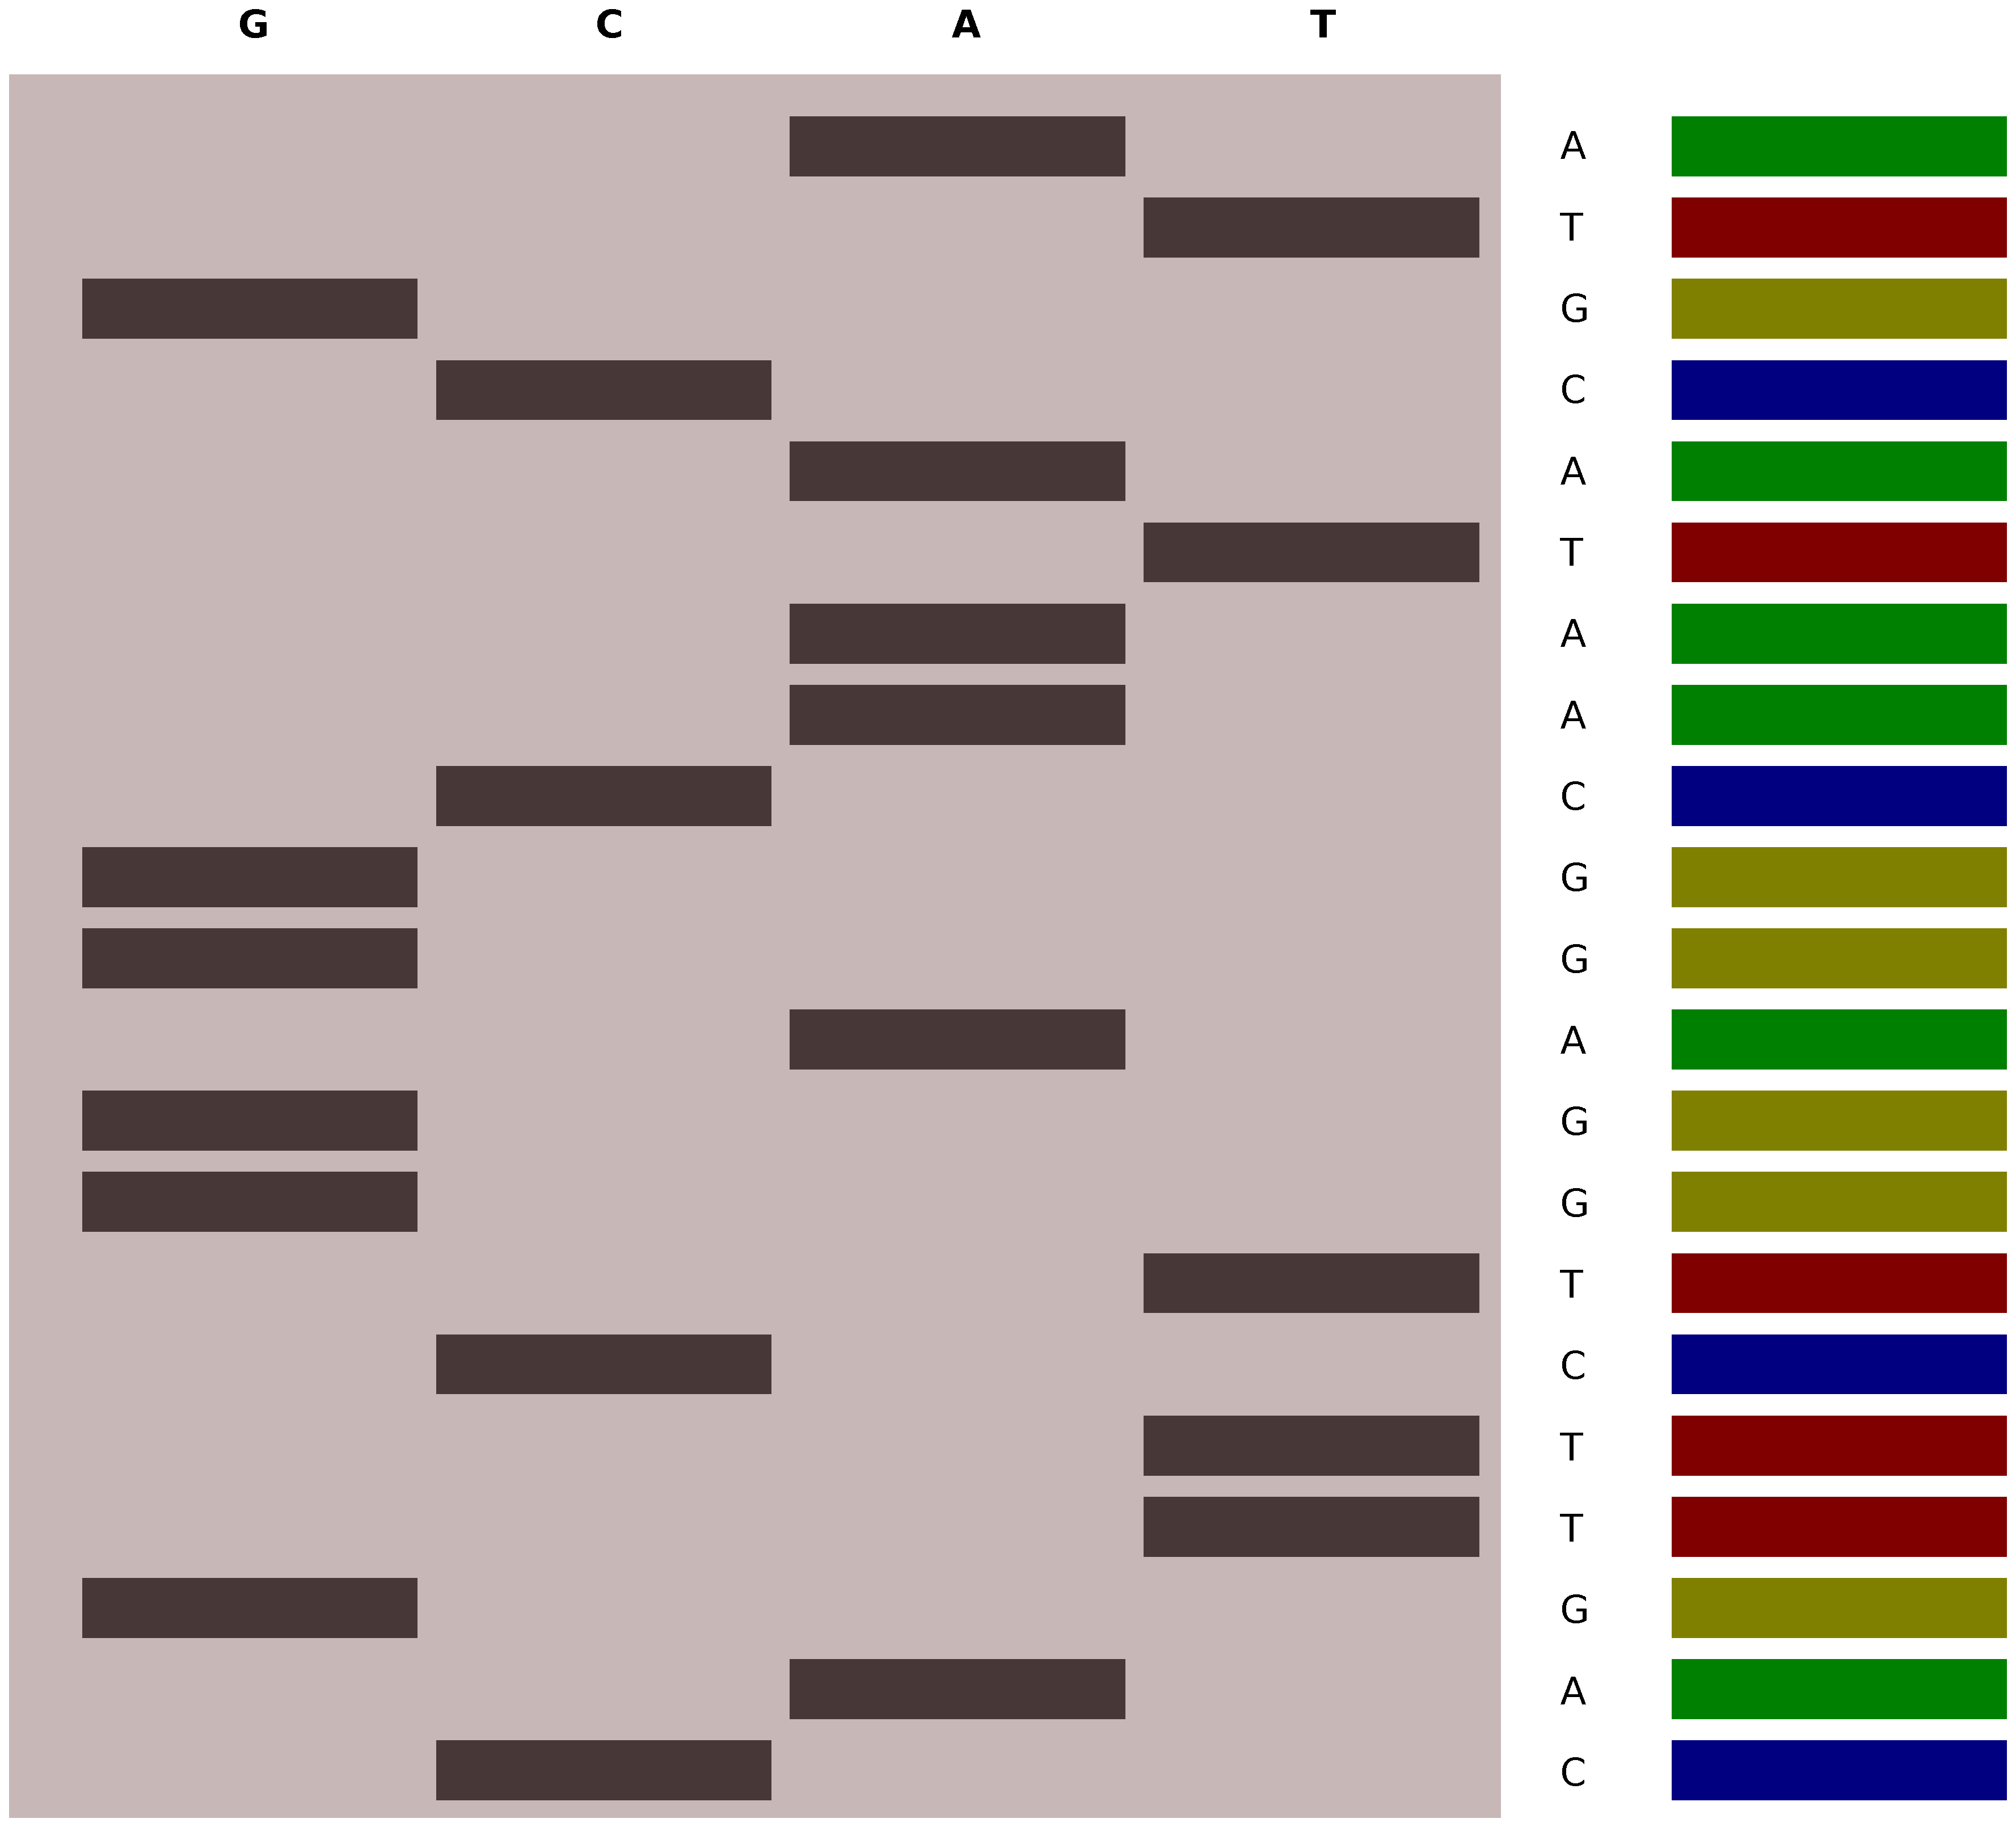
\includegraphics[width=0.8\textwidth]{illumina/sanger.pdf}}
\caption{Schematic of Sanger Sequencing using terminator chemistry. Left: sequencing on a four-lane gel. Four lanes represent sequencing mixtures containing different ddNTPs. Right: Sanger sequencing in a single lane using fluorescently labelled ddNTPs. Middle: the corresponding DNA sequence.}
\label{fig:sanger}
\end{figure*} 

\paragraph{Illumina Sequencing Technology}
The most popular, and best known, NGS technology is Illumina's sequencing by synthesis~\cite{illumina2010}. In the Illumina sequencing pipeline, DNA strands are fragmented into short pieces and attached to specific adapter sequences. The modified sequences are introduced to the Illumina flowcell, locally amplified in a ``clustering" reaction~\cite{Adessi2000} and then cycled through repeated elongation and imaging steps, to read out the DNA sequence one nucleotide at a time (Fig.~\ref{fig:illumina}). Illumina sequencing is a fluorescence-based technology. It uses reversible terminator chemistry to elongate a templated DNA molecule by a single base, using a dye-labelled nucleotide bearing a terminator group to prevent further elongation. The DNA base is identified based on the fluorescence emission of the attached dye. Following imaging, the terminator group and dye are removed and the next terminated nucleotide introduced at the now exposed hydroxyl group (Fig.~\ref{fig:terminator}). 

\begin{figure*}
\centerline{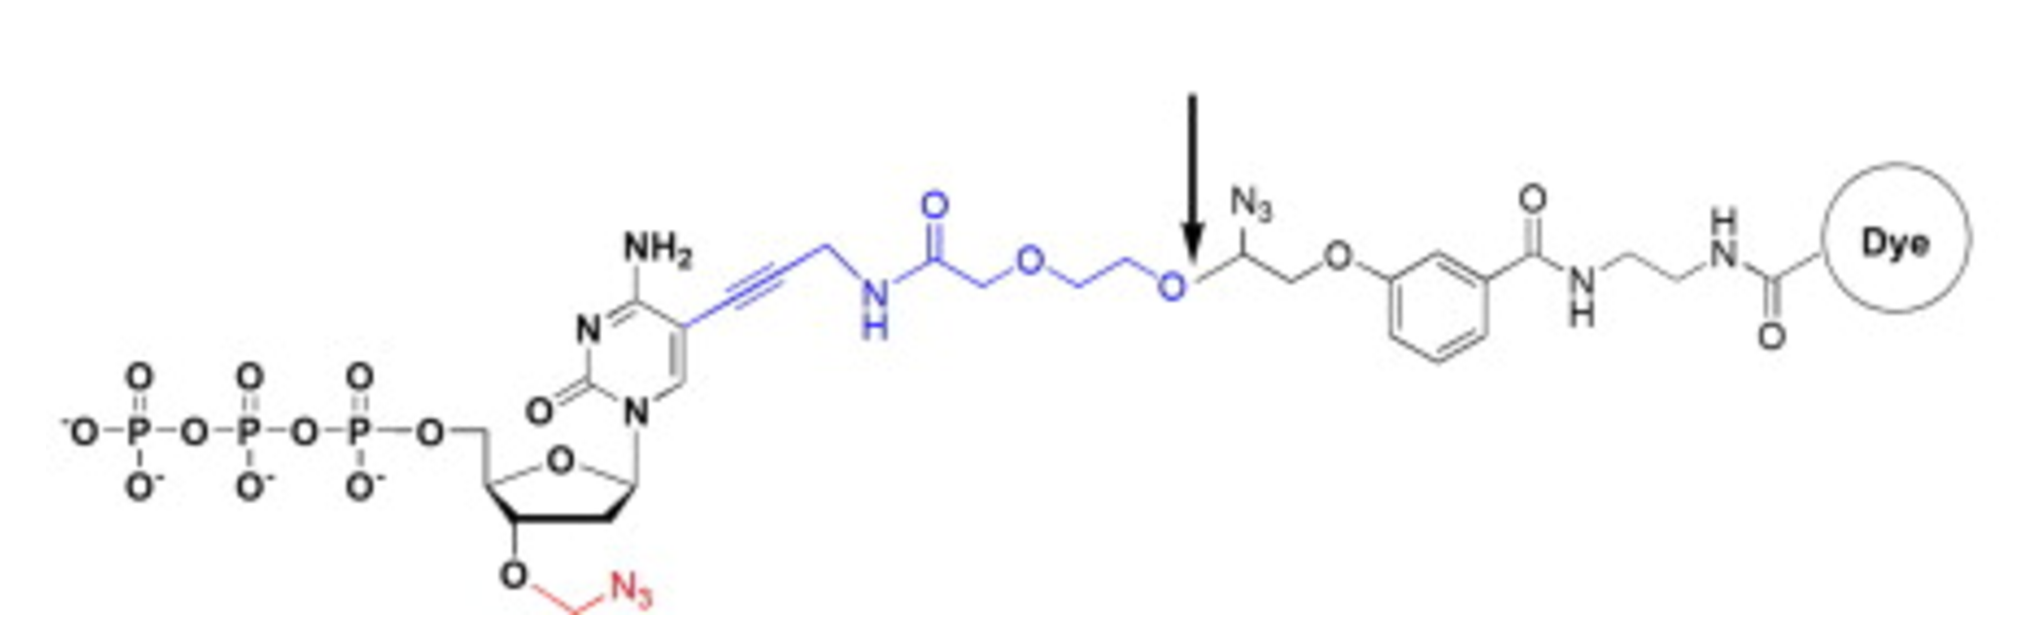
\includegraphics[width=0.8\textwidth]{illumina/illumina_linker.pdf}}
\caption{A modified nucleotide showing Illumina terminator chemistry. The 3'-hydroxyl group is reversibly blocked by the 3′-O-azidomethy terminator (red atoms), whilst the fluorescent indicator dye can be reversibly cleaved from the modified DNA base at the bond indicated by the arrow. Figure adapted from~\cite{Chen2013}}
\label{fig:terminator}
\end{figure*}  

This is a fluorescence based imaging technique. However, there are several major differences between this sequencing process and the single molecule confocal experiments described in the previous chapters. Firstly, rather than freely diffusing molecules imaged by a laser beam, the fluorescently labelled sequences are tethered to the flow-cell base and imaged using multiple cameras and epifluorescent illumination (see Section~\ref{subsect:techniques}). Secondly, unlike in a smFRET experiment, the imaging step does not attempt to distinguish individual fluorophores against a noisy background signal. Instead, the clustering step prior to imaging produces multiple, spatially localised copies of the same DNA sequence, hugely amplifying the available fluorescent signal. 

\begin{figure*}
\centerline{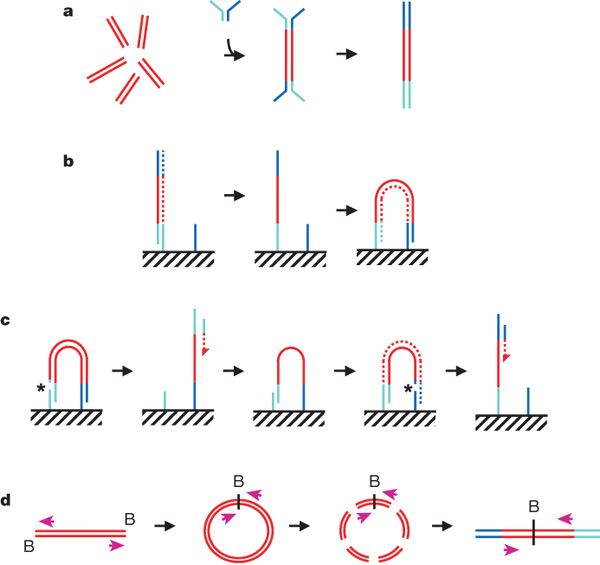
\includegraphics[width=0.8\textwidth]{illumina/illumina_sequencing.jpg}}
\caption{Sequencing by synthesis. A) DNA fragments are generated and joined to a pair of oligonucleotides. The ligated products are amplified using two oligonucleotide primers, resulting in double-stranded blunt-ended material with a different adaptor sequence on either end. B) DNA fragments are denatured and single strands are annealed to complementary oligonucleotides on the flow-cell surface. A new strand is copied from the original strand in an extension reaction; the original strand is then removed by denaturation. Multiple cycles of annealing, extension and denaturation in isothermal conditions result in cluster growth. C) The DNA in each cluster is linearized by cleavage within one adaptor sequence and denatured, generating single-stranded templates. D) Long-range paired-end sample preparation. The ends of each long fragment are tagged by incorporation of biotinylated (B) nucleotide and then circularized, forming a junction between the two ends. Circularized DNA is randomly fragmented and the biotinylated junction fragments are recovered and used as starting material in the standard sample preparation procedure. Figure and (adapted) caption from~\cite{bentley2008}.}
\label{fig:illumina}
\end{figure*} 

\paragraph{Single Molecule Sequencing Technologies}
Although Illumina does not use single molecule imaging, several other sequencing methods do sequence individual DNA molecules. Single Molecule Real Time Sequencing (SMRT)~\cite{eid2008} is another fluorescence based sequencing technology. In SMRT, DNA polymerase molecules are immobilized within the detection region of a zero-mode waveguide (ZMW). Fluorescently labelled dNTPs are incorporated by the polymerase and imaged in real time. The ZMW, an aluminium-coated glass slide, containing multiple nano-scale pinhole apertures, creates a zeptolitre detection volume, enabling detection of the nucleotide currently under incorporation, despite a relatively high ($\mu$M) concentration of labelled oligonucleotides~\cite{Levene2003}. SMRT, used in Pacific Biosciences sequencing technologies, is currently extremely expensive, but produce sequences with an average read length of 3000 nucleotides~\cite{Roberts2013}, compared with the 151 or 251 bases typical of an Illumina read.

A second, currently experimental, single molecule sequencing technique is under development by Oxford Nanopore~\cite{Bayley2014}. This sequencing method uses electrophoresis to drive long DNA molecules through a nano-scale pore. Application of a voltage across the nanopore causes a flow of ions through the pore, creating a measurable current. DNA is negatively charged, so can also be drawn through the pore, causing variations in the observed current that are dependent on the DNA bases currently occupying the pore~\cite{Branton2008}. In principle, this allows a direct read-out of the base sequence; in practice several challenges, including control of the speed of strand progression through the pore and achieving individual base resolution~\cite{Laszlo2014}, mean that although nanopore sequencing can produce very long reads (average 5000 bases), these have a high error rate including systematic errors~\cite{Mikheyev2014}.  

\subsection{De Novo Sequence Assembly}
As described above, Illumina NGS produces reads of length 151 or 251 bases. Even a small bacterial genome has a total genomic size of several million bases. Consequently, one of the most challenging aspects of genome sequencing is to piece together the short fragments of sequence obtained from the sequencer into one or more contiguous sequences, corresponding to correctly reconstructed sections of the genome. This process of attempting to generate a complete genome from short reads is termed \textit{de novo} sequence assembly; it is distinct from, for example, sequence alignent~\cite{Li2010}, in which short reads are aligned against a previously constructed reference genome for the same organism, allowing identification of polymorphisms and small differences from the reference genome. 

\textit{De novo} assembly is the construction of a long, contiguous genomic sequence from short DNA reads, without using a reference genome. The most popular method of \textit{de novo} assembly contstructs a de Bruijn overlap graph~\cite{Compeau2011} from even shorter fragments, termed $k$-mers, generated by fragmenting the short reads, then traverses this graph to reconstruct the genome sequence. De Bruijn graph traversal as a method of assembly was proposed as early as 2001~\cite{Pevzner2001}; however the method only gained popularity once the first de Bruijn assemblers were released~\cite{Zerbino2008}. In the simplest case, the graph is constructed from single end reads. However, with only single end reads, disambiguating repeat regions, which tangle the de Bruijn graph, remains challenging. 

In de Bruijn graph assembly, the sequencing reads are subdivided into all possilbe shorter reads of length $k$, termed $k$-mers. A $k$-mer is described as having a prefix (the first $k - 1$ nucleotides) and a suffix (the last $k - 1$ nucleotides). A graph is then constructed, in which observed prefixes and suffixes are represented as nodes; a directed edge is drawn between two nodes if the $k$-mer representing that prefix-suffix pair is present in the sequencing data (Fig.~\ref{fig:de-bruijn}). The challenge of constructing the \textit{de novo} assembly is then addressed by constructing a continuous path through the resulting de Bruijn graph, in which every edge is visited. Such a path is termed an Eulerian cycle; efficient algorithms exist to find such cycles and many have been implemented for the \textit{de novo} assembly application~\cite{Zerbino2008, Bankevich2012, Li2010_SOAP}. 

\begin{figure*}
\centerline{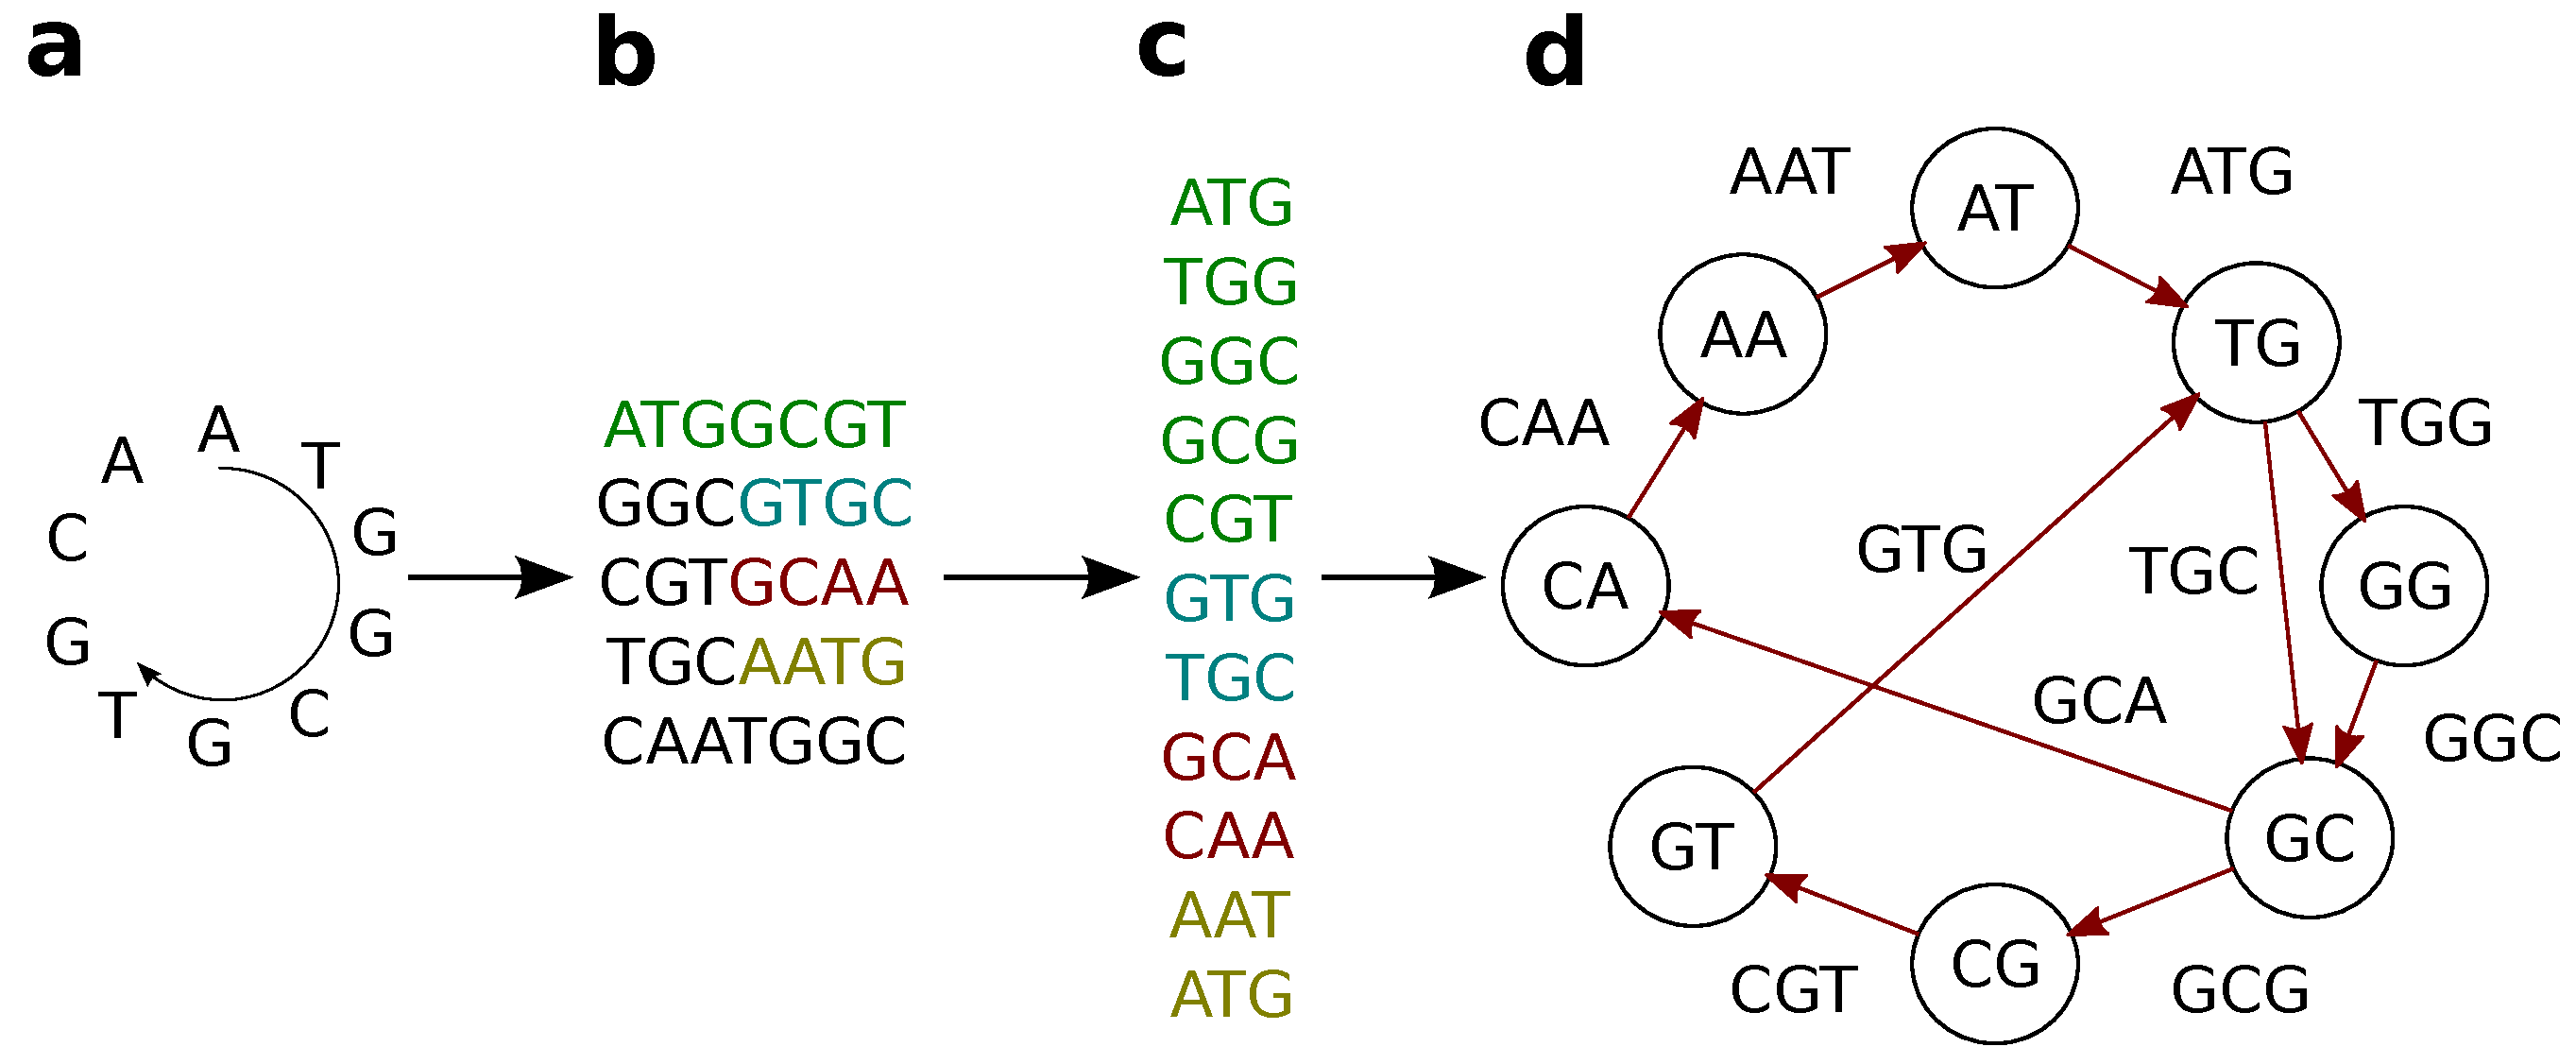
\includegraphics[width=0.8\textwidth]{illumina/de_bruijn.pdf}}
\caption{De Bruijn graph assembly from $k$-mers. (A) A small, circular genome (B) Some short reads sequences. (C) Breaking the reads into $k$-mers ($k = 3$). $k$-mers are coloured according to the sequence from which they are derived. (D) Constructing a De Bruijn Graph from the $k$-mers. Figure adapted from~\cite{Compeau2011}.}
\label{fig:de-bruijn}
\end{figure*}

Even using the most sophisticated assemblers, it is rare for the entire genome to be recovered as a single, contiguous unit. Consequently, assembly is typically a two-stage process. First, long contiguous sections, named contigs, are constructed. Second, once the contigs cannot be extended any further, ``scaffolding" algorithms~\cite{hunt2014} attempt to join multiple contigs, using insert size information to determine contig order and approximate gap size.

One important challenge that is not resolved by de Bruijn graph assembly is the disambiguation of repeats -- sequences found in multiple places in the genome -- which tangle the de Bruijn graph (Fig.~\ref{fig:tangle}): certain $k$-mer sequences, corresponding to the start and end of repeat regions, have multiple entry and exit paths, the ordering of which cannot be determined. Repeat disambiguation is a major challenge for correct \textit{de novo} assembly. Consequently, several alterations to the sequencing methodology have been developed to provide more data about the positioning of repeat sequences within a genome. 

\begin{figure*}
\centerline{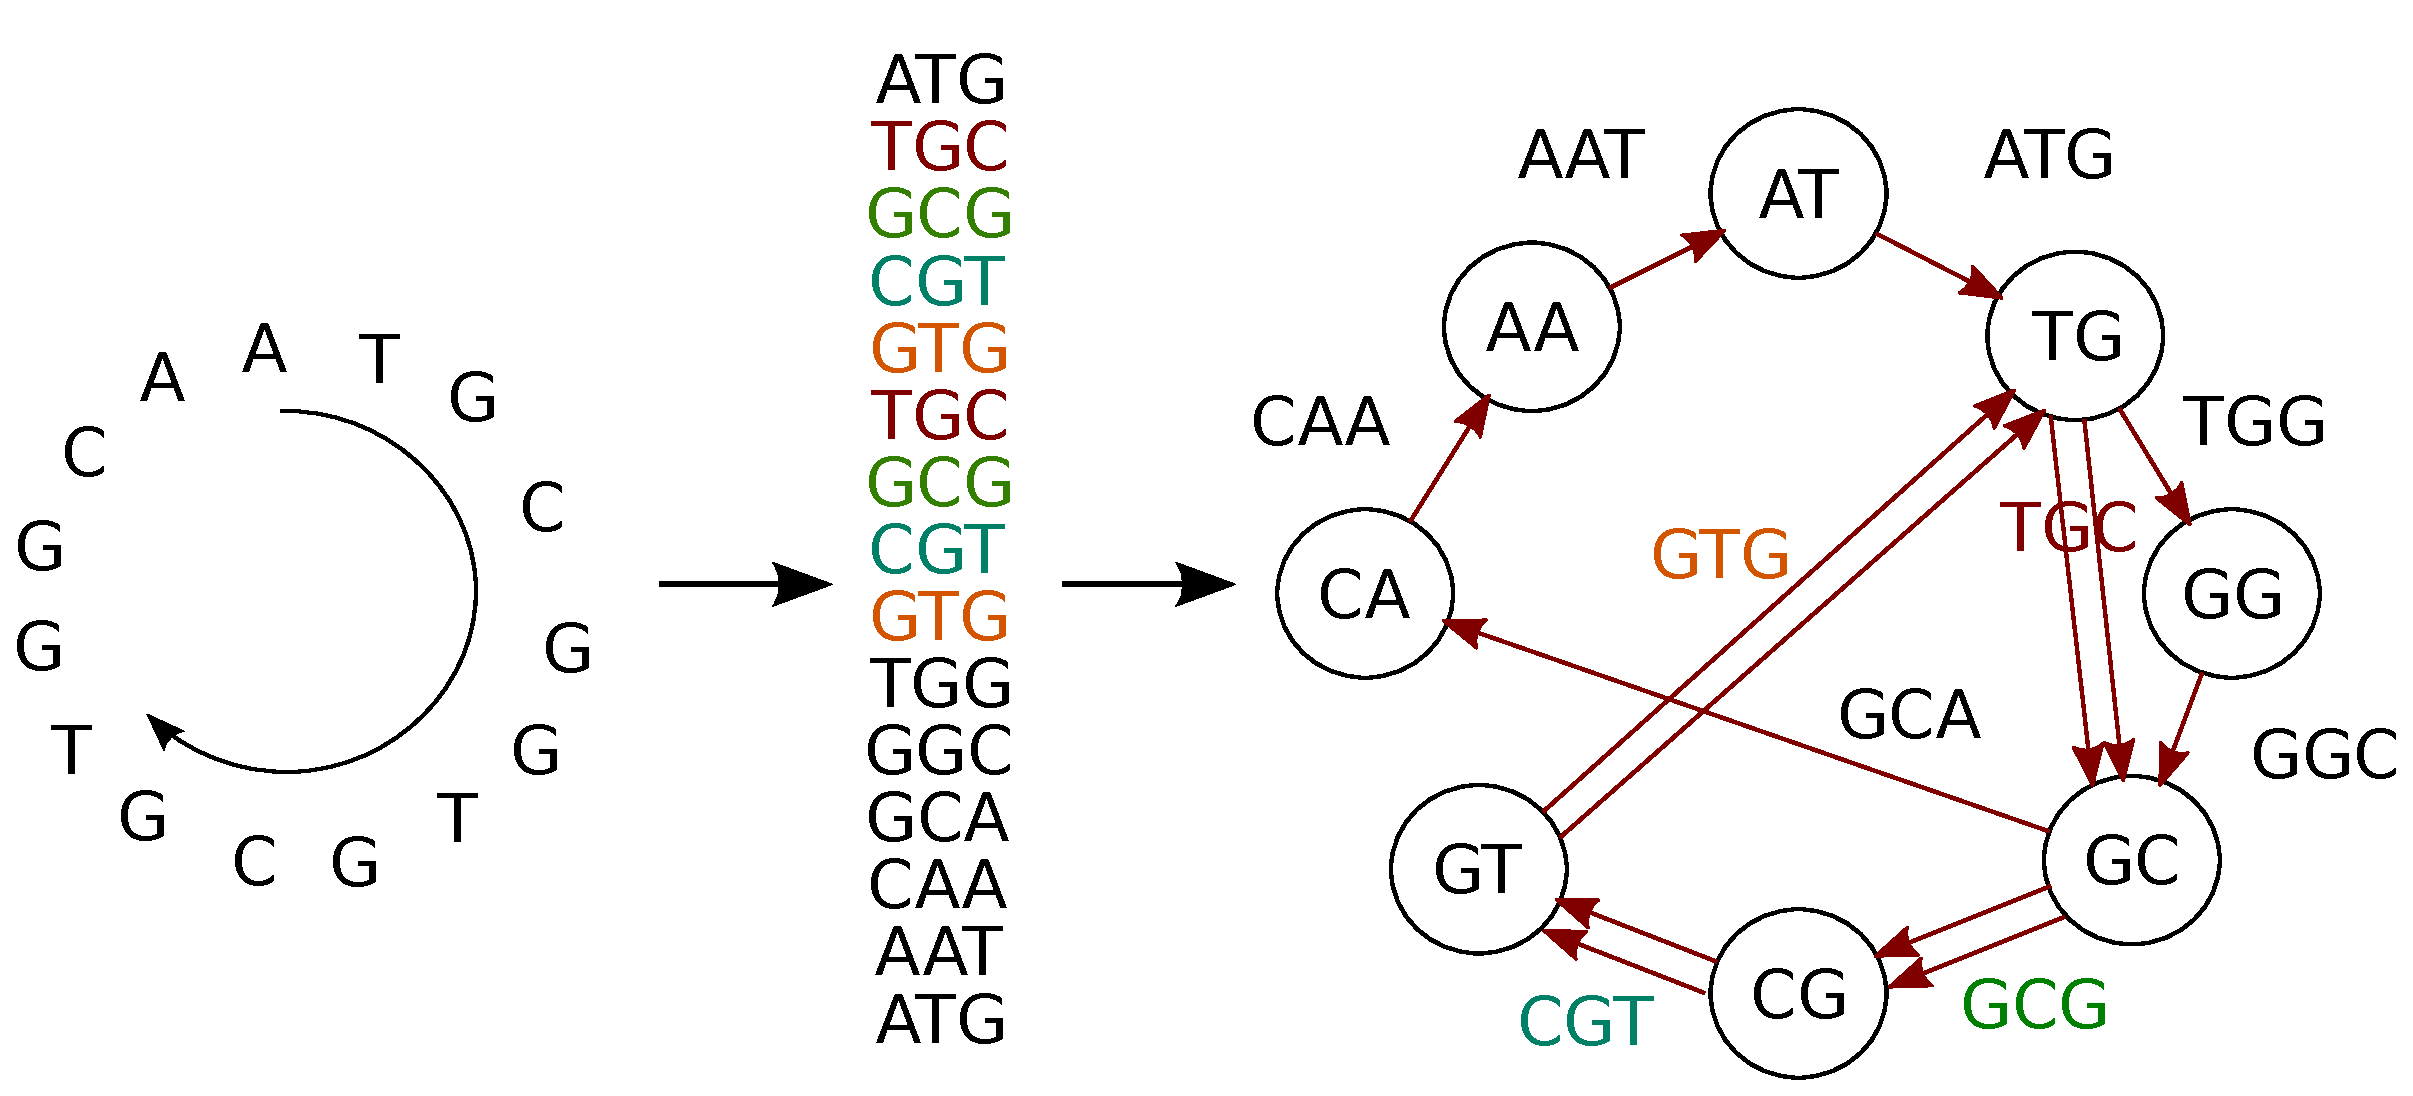
\includegraphics[width=0.8\textwidth]{illumina/de_bruijn_tangle.pdf}}
\caption{A se Bruijn graph with repeats. The larger circular genome ATGCGTGCGTGGCA contains the repeated section TGCGTG, resulting in several 3-mers (TGC, GCG, CGT and GTG, coloured red, green blue and orange respectively) appearing more than once. This results in a tangled de Bruijn graph. Figure adapted from~\cite{Compeau2011}.}
\label{fig:de-bruijn}
\end{figure*}

\subsection{Paired End Reads and Mate Pair Sequencing}
\paragraph{Paired End and Single End Reads}
The description of \textit{de novo} assembly given above has assumed that reads are ``single-end" -- that is, the fragments of genomic DNA attached to the flowcell surface are sequenced using one strand only. However, a simple modification to the protocol additionally allows sequencing of the complementary strand. This provides two sequences, corresponding to the two ends of the genome fragment, separated by some unsequenced central region. These two sequences can be matched~\cite{edwards1990}, to give a pair of reads (a read pair), separated by some small distance within the genome. The genomic distance from the start of one read to the end of the other is termed the insert size. The genomic libraries used for this paired end sequencing typically contain fragments with an insert size of around 500 bases in length, although this can be controlled during library preparation.

When the insert size (fragment length) is longer than the length of a repeat unit, paired end reads provide extra information that can help to disentangle a de Bruijn graph. By creating a bridge between the start and end sections of a repeat unit, the paired end reads can enable the order of repeat sections to be determined. Some assemblers~\cite{medvedev2011, Bankevich2012} directly incorporate pairing information into the de Bruijn graph; in other assembly pipelines, pairing information is used in the subsequent  scaffolding step to order determine the correct ordering of the contigs.  

\paragraph{Mate Pair Sequening}
Many repeat regions are larger than the average insert size of a paired end library, with the result that fully constructing a genome from short reads is still not possible. To enable further disambiguation of the repeat structure, protocols to create read pairs with a much larger insert size have been developed~\cite{nextera2012}, allowing construction of libraries containing fragments that are several kilobases (kb) in length. These ``mate pair" libraries can be used either alone, or in combination with a paired end library, to provide additional information for a \textit{de novo} assembly.

\subsection{Evaluating Assembly Quality}
Many assemblers incorporate mate pair insert size information into either both the contig assembly and scaffolding processes~\cite{medvedev2011, Bankevich2012}, or just into the scaffolding step~\cite{Zerbino2008} but errors can still occur. These errors can significantly affect the quality of the assembled genome, with repercussions for downstream research. Consequently, error correction and quality evaluation of \textit{de novo} assemblies are problems receiving considerable research interest.

The most serious mistakes found in a \textit{de novo} assembly are large scale scaffolding or extension errors (Fig.~\ref{fig:NxRepair} (A)), in which two two disparate regions of a genome are incorrectly joined together. Similarly, large insertion or deletion errors (indels) create structural irregularities in the \textit{de novo} assembly; whereas mistakes in base calling lead to errors at a single position only. 

The most common method of evaluating assembly quality is to measure its $N50$ score, defined as ``the length of the shortest contig in the set that contains the fewest (largest) contigs whose combined length represents at least 50\% of the total assembly"~\cite{Miller2010}. However, this evaluation method optimises only for contig length, without considering the correctness of the assembly. When a reference genome is available, the modified $NA50$ statistic~\cite{Gurevich2013} can be used, which considers only contig sections that correctly align to the reference. Recent work, such as the Assemblathon~\cite{Bradnam2013} and GAGE~\cite{Salzberg2012} collaborations used this metric to compare the quality of the \textit{de novo} assemblies prepared by various assemblers by comparing them with their equivalent reference genomes. However, in the absence of a high-quality reference genome, other methods of quality evaluation must be used.

\subsection{Error Detection Methods}
Ghodsi et al.~\cite{Ghodsi2013} have developed a Bayesian method of assembly quality evaluation, which can calculate an assembly quality score, without requiring a reference genome. However, this provides only an overall quality score and cannot be used to identify errors or low-quality regions. Several recent papers have developed error identification and correction methods, which perform a fine-grained analysis of assembly quality. The most well-known of these is the A5 Assembly Pipeline~\cite{Coil2014, tritt2012}, which includes an error detection and rescaffolding step that makes use of mate pair alignment information. Two new tools, REAPR~\cite{Hunt2013} and ALE~\cite{Clark2013} have also been developed to use read pair data to identify misassemblies. A similar tool is currently under development at the Broad Institute~\cite{pilon2014}. However, with the exception of ALE, which is no longer actively maintained, these newer tools are not optimised to use mate pair information.  

This chapter describes NxRepair, an assembly error detection tool that we designed to identify the most serious misassemblies by examining the distribution of Nextera mate pair insert sizes. NxRepair does not require a reference genome and can be used with assemblies prepared with a single mate pair library alone. It specifically targets the most serious scaffolding errors and large-scale indels by identifying regions with a high number of anomalous insert sizes, or very few supporting reads, breaking the scaffold and optionally trimming out the misassembled region. NxRepair also provides a fine-grained quality score, allowing researchers to visualise poor-quality regions. 

In the following sections, we describe the theoretical basis of NxRepair and its efficient implementation using an interval tree data structure. We then demonstrate the use of NxRepair on bacterial genomes assembled from a single Nextera mate pair library. For the \textit{de novo} assembly process, we use the state of the art SPAdes assembler~\cite{Bankevich2012}, which explicitly uses insert size information during contig construction, as well as for scaffolding. Using these genomes, we benchmark NxRepair against the error correction module of the A5 assembler, A5qc~\cite{tritt2012}, which is currently the most widely used error correction tool, demonstrating NxRepair's superior performance. We conclude the chapter with a discussion of the performance and limitations of NxRepair as a quality control tool and discuss possible extensions that could improve performance.

\begin{figure*}
\centerline{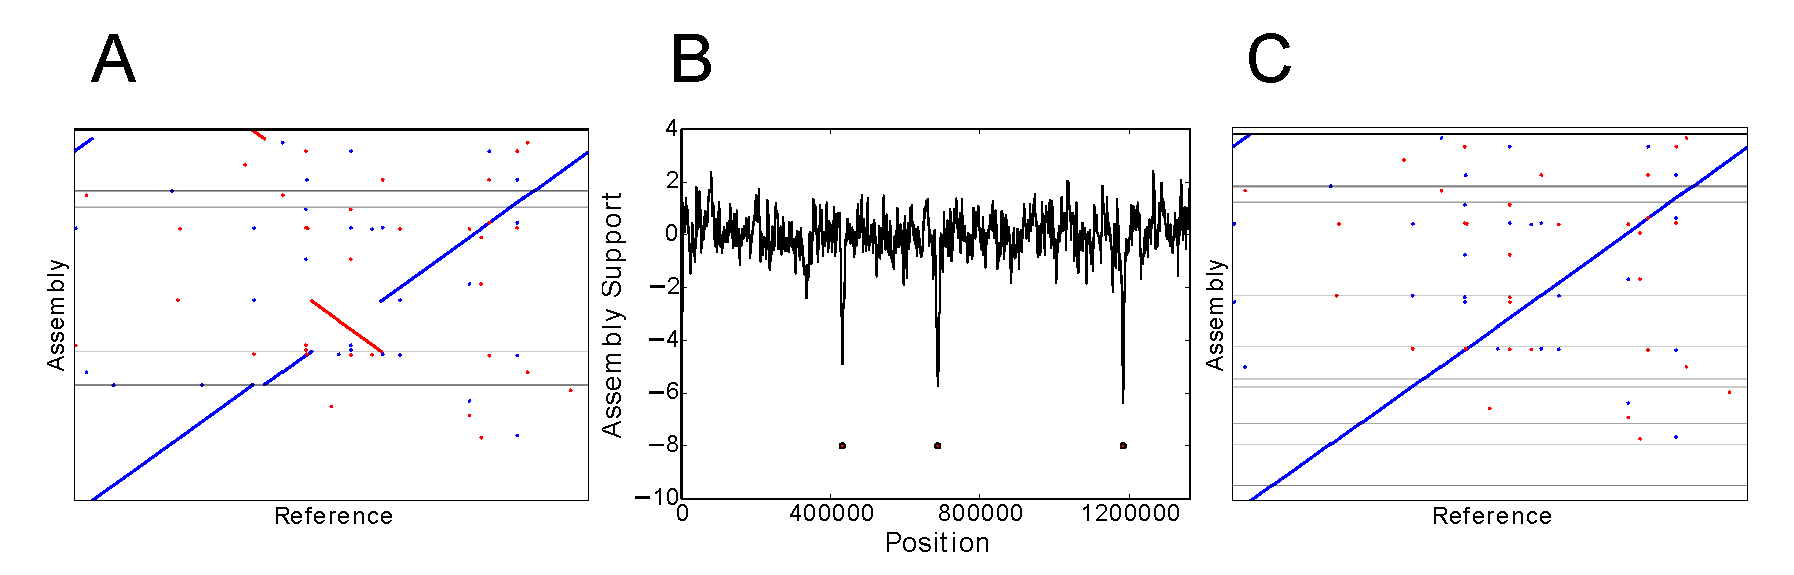
\includegraphics[width=0.8\textwidth]{illumina/fig1_nxrepair.pdf}}
\caption{Using NxRepair to remove large misassemblies. (A) Alignment of the \textit{de novo} assembly of the M. tuberculosis genome to its reference genome. The assembly contains several large misassemblies. (B) A plot of NxRepair's support metric against scaffold position for the assembly. Low support for the assembly is identified in three regions of a contig. (C) Breaking the contigs at the identified positions resolves the most significant misassemblies. In (A) and (C), horizontal lines demarcate the scaffold boundaries.}\label{fig:NxRepair}
\end{figure*}

\clearpage

\section{Theory}
\subsection{Statistical Analysis of Mate Pair Insert Sizes}
\label{sect:illumina_theory}
Nextera mate pair libraries are prepared to have a certain insert size, typically between 1 and 10 kb. Following construction of a \textit{de novo} assembly, it is possible to align the mate pair reads used to construct the assembly back to the assembly itself. The actual distance along the \textit{de novo} assembly between the two reads that form a mate pair can then be calculated. Large-scale errors in the assembly will cause mate pair reads aligning near to the error to have unusual insert sizes and read orientations. This means that we can use the insert size distribution displayed by mate pair reads aligning at different sites along the assembly to evaluate the local assembly quality. We identify assembly errors at sites where the local insert size distribution deviates too far from that observed in the rest of the genome.       

We model the observed insert sizes of mate pairs aligned to the \textit{de novo} assembly using a two-component mixture distribution. The first component of this mixture is the insert size distribution of correctly aligned mate pairs.  We model the distribution of insert sizes, $Y$, as a normal distribution with mean $\hat{\mu}$ and standard deviation $\hat{\sigma}$: $Y \sim N(\hat{\mu},\hat{\sigma}^2).$ We estimate $\hat{\mu}$ and $\hat{\sigma}$ for the entire genome by aligning reads back to the assembly and using robust estimators (see below). The second component, defined as a uniform distribution across the contig size $U(0,L)$ for a contig of length $L$, captures anomalous insert sizes. 

To calculate the degree of support for the assembly at each site across a contig, NxRepair retrieves all mate pairs spanning the region $[i-W, i+W]$, of size $2W-1$ at position $i$ on the contig, where spanning is defined to mean that one read ends entirely before the region $[i-W, i+W]$ and the other read begins entirely after (see Fig.~\ref{fig:spanning}.) The default value of $W$ is 200 bases (see Table~\ref{tab:parameters}). 

A uniform distribution was selected to model anomalous insert sizes, as it makes no assumption about the cause of an anomaly. It is uniform over the contig length, $L$, as opposed to over all possible sites in the assembly, as only pairs where both members align fully to that contig are considered. Similarly, even though the insert size distribution for correctly aligned mate pairs will typically display a longer tail than the normal distribution (unless a gel-extraction protocol is used), we found that using a normal distribution to model correct insert sizes did not adversely affect NxRepair's error detection. This is because each site is spanned by many mate pairs and the insert size of correctly aligned mate pairs is not correlated with location. Consequently, despite these assumptions, the small fraction of correctly aligned mate pairs with a very large insert size do not lead to false positives in error identification. 

We define a latent indicator variable $X_l\in\{0,1\}$ for each pair of reads, $l$, which takes the value $1$ if the insert size came from the null distribution, and $0$ otherwise. Within each window queried, the probability that each retrieved read, $r_l$ is drawn from the null distribution is given by:

\begin{eqnarray} P(X_l=x|Y_l)& =& \frac{\pi_x(Y_l|X_l=x)}{\sum_{k=0}^1 \pi_k(Y_l|X_l=k)}
\label{eq:posterior}  
\end{eqnarray}

where $Y_l$ is the insert size of read pair $l$, $\pi_k$ is the user defined prior probability of class $k$ and $\pi_1 + \pi_0 = 1$. The default value of $\pi_0$ is 0.01 (see Table~\ref{tab:parameters}), meaning that in the absence of any insert size information, 99 \% of read pairs are expected to arise from the null distribution.  

Within each window, the total support for a correct assembly at position $i$ can be calculated as:

\begin{equation}
D_i = \sum_{l=1}^N P(X_l=1|Y_l)\cdot C_l
\end{equation}

where the summation is over all read pairs aligning across position $i$ and $C_l$ is an indicator variable, reporting pairing orientation:

\begin{equation}
    C_l=
    \begin{cases}
      1, & \text{if}\ \text{mate pairs have correct orientation and strand alignment} \\
      0, & \text{otherwise}
    \end{cases}
  \label{eq:C}
  \end{equation}

Within each contig, the contig assembly support mean $\mu_D$ and variance $s_D$ are calculated from all reads aligning to the contig,
\begin{equation}
\hat{\mu}_D = \frac{\sum_{l=1}^N D_l}{N} \qquad s_D = \frac{\sum_{l=1}^N \sqrt{(D_l - \hat{\mu})^2}}{N}
\label{eq:contigD}
\end{equation}

We use these contig specific mean and variance, rather than the global values, to prevent local variations in coverage from either causing false positives or masking changes in the insert size distribution. Using these values, we calculate the Z-score $z_l$ within each queried interval as: 

\begin{equation}
z_l = \frac{D_l - \hat{\mu}_D}{s_D}
%\hat{\mu} = \frac{\sum_l^N D_l}{N} \qquad \s = \frac{\sum_l^N \sqrt{(D_l - \hat{\mu})^2}}{N}
\label{eq:zscore}
\end{equation}

The Z-score is sensitive both to local changes in the insert size distribution, and to large variations in the number of correctly aligned mate pairs, for example caused by a large number of reads with a mate aligning to a different contig. This ensures that NxRepair can identify misassemblies occurring both within and between contigs.  

A misassembly is identified if $z_l < T$ for a user-defined threshold $T$ (default value -4). This threshold describes the number of standard deviations below the mean assembly support that is required to identify an anomaly. The default value of -4 will flag only positions whose assembly support is less than four standard deviations below the mean level of support.

\begin{figure}
\centerline{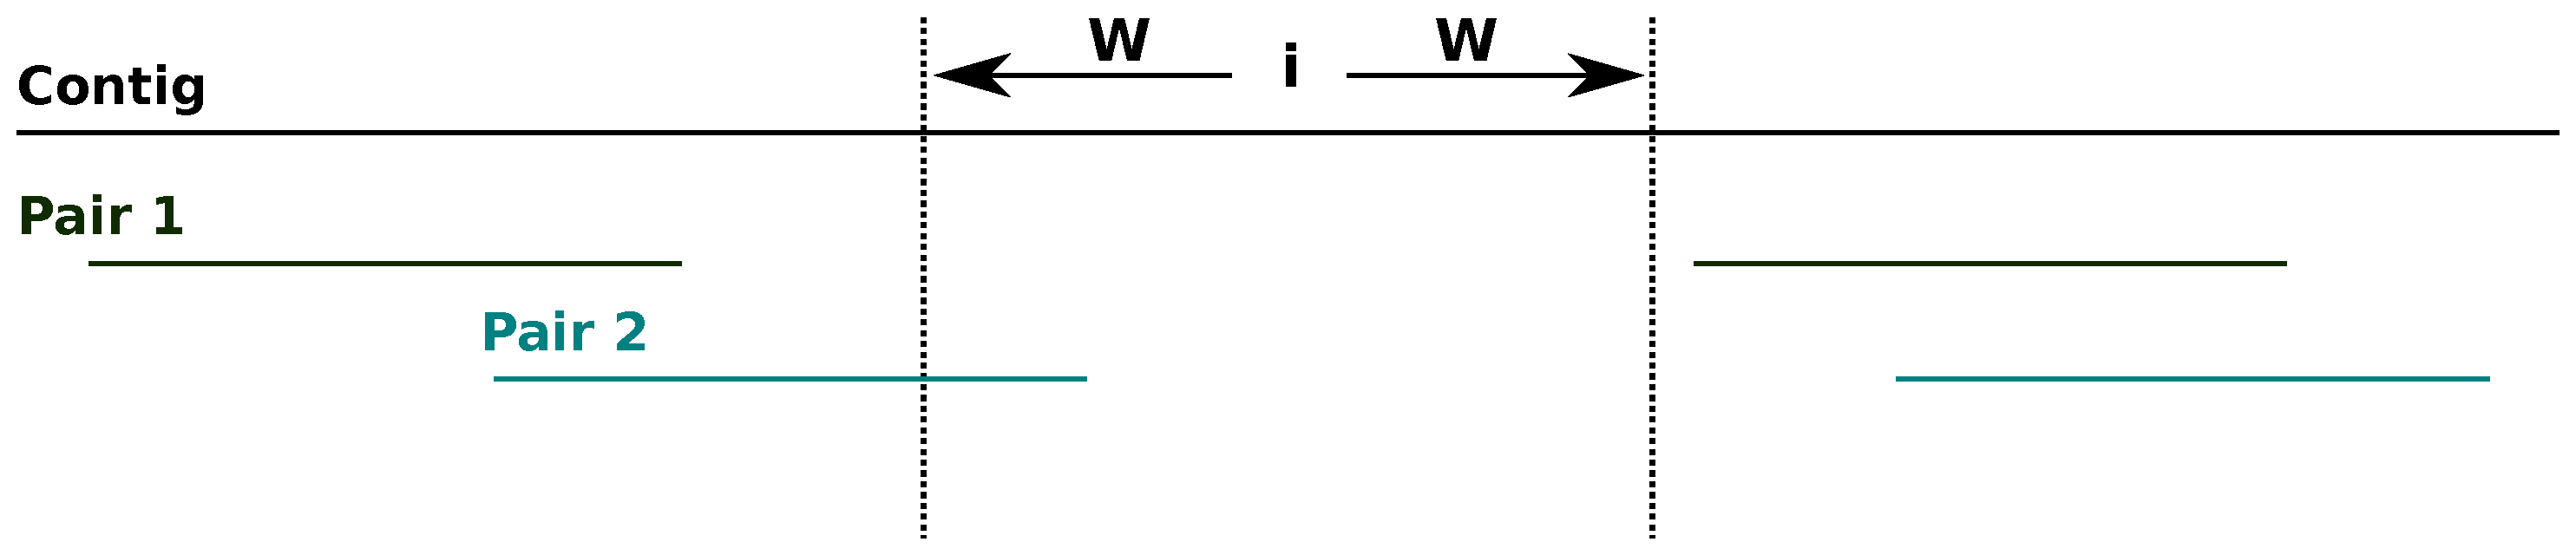
\includegraphics[width=0.8\textwidth]{illumina/spanning.pdf}}
\caption{Schematic illustrating mate pairs spanning a selected region. The upper read pair (green) spans the indicated region, as both reads align entirely outside of the region $[i-W, i+W]$. The lower read pair (cyan) do not span the indicated region, as the left-hand read overlaps the target area. \label{fig:spanning}}
\end{figure}

\subsection{Global Assembly Parameters}
NxRepair identifies misassemblies by identifying regions where the mate pair insert size distribution differs significantly from the insert size distribution across the entirety of the \textit{de novo} assembly. Consequently, it is necessary to have a robust estimate of the global mate pair insert size distribution. For calculation of population statistics, mate pairs that align to different contigs are excluded, as are mate pairs with an incorrect strand or pairing orientation and pairs whose insert size exceed 30 kb (approximately 10 times the mean insert size). Pairs whose mapping quality falls below a user specified threshold (minmapq, default value 40) are also excluded, removing reads that are not uniquely mapped from the calculation of global parameters. The global mean $\hat{\mu}$ and median absolute deviation ($\text{MAD}$) are calculated across all contigs in the assembly as:

\begin{equation}
\hat{\mu} = \frac{\sum_{l=1}^N Y_l}{N} \qquad \text{MAD} = \text{median}_m(|Y_m - \text{median}_l(Y_l)|)
\label{eq:global}
\end{equation}

where $\text{median}_l(Y_l)$ is the median insert size of reads with correct pairing behaviour and $|Y_m - \text{median}_l(Y_l)|$ is the absolute value of the residual from the median of the $m$th on $N$ reads. The standard deviation was then calculated by scaling the MAD using:

\begin{equation}
\hat{\sigma} = K \cdot \text{MAD}
\label{eq:mad_to_sigma}
\end{equation}

where 

\begin{equation}
K = \frac{1}{\frac{3}{4} \cdot \phi^{-1}} \sim 1.4826
\label{eq:k_scale}
\end{equation}

and $\phi^{-1}$ is the quantile function~\cite{Leys2013}

The $\text{MAD}$ is a robust estimator for the standard deviation, as it is not sensitive to outliers, such as the long tail of the mate pair insert size distribution. Using the MAD as an estimator prevents over-estimating the variance of the insert size, allowing anomalously large insert sizes to be correctly identified.

These were then used as the parameters of the null distribution, as described above (Section~\ref{sect:illumina_theory}.

\subsection{Interval Tree Construction}
To facilitate rapid lookup of mate pair properties, we construct an interval tree~\cite{cormen2009} for each contig in the \textit{de novo} assembly. An interval tree is a data structure that facilitates $O(\text{log} n + m)$ lookup of intervals that span a given point or interval, for $n$ total entries and $m$ spanning entries. The interval tree contains the start and end positions of each mate pair aligned to that contig, as well as a flag variable indicating whether that mate pair had correct strand and pairing orientation. Mate pairs where the two reads align to different contigs were excluded. Mapping quality is currently not considered at this stage - reads are retained regardless of mapq score. For each position $i$ for which the Z-score is to be calculated, the tree is queried with a start position $i-W$ and end position $i+W$, to retrieve read pairs spanning the interval between positions $i-W$ and $i+W$ (exclusive). The insert sizes of retrieved read pairs are then used to calculate the Z-score for position $i$. This allows NxRepair to rapidly query positions across a contig to discover the insert size distribution at the queried position. Use of the interval tree significantly increases the efficiency of Z-score calculation, as each pair of reads is fetched only once in order to build the tree. All relevant parameters are then stored in the tree for rapid look-up when a position is queried. This has several advantages. Firstly, it is significantly faster than fetching reads only when a position is queried. Secondly, it is more space efficient than a frequency array of all positions on all contigs but does not lose any information about the exact alignment positions. Finally, once construction of the tree is complete, multiple passes across a contig (for example with different spatial resolutions, or using different window sizes) can rapidly be made using the same tree.      

\subsection{Misassembly Location and Contig Breaking}
To improve the quality of the \textit{de novo} assembly, once a misassembly has been located, a contig is broken into two separate pieces at the site of a misassembly. The broken ends of the two new contigs can optionally be trimmed by a user defined length (default 4 kb) to remove the misassembled region. Trimming allows removal of the incorrectly assembled regions around a break-point, but can be switched off if a user does not want any sequence to be removed from the assembly. To prevent excessive clipping, misassemblies separated by less than the trimming distance are grouped together, the contig is broken at the start and end of the misassembled region and the misassembled section is discarded. Low-scoring regions within the trimming distance of the ends of contigs are not considered misassemblies, as the high proportion of mate pairs aligning here whose mate maps to a different contig reduces the number of pairs under consideration and hence lowers the observed Z-score. This also ensures that circular molecules, such as small plasmids, which are assembled into a single contig, are not truncated because of mate pairs at either end of the assembly that appear to span the entire contig, but which are spatially close when circularisation is considered.

\subsection{Availability and Dependencies}
NxRepair is available for free anonymous download from the Python Package Index (PyPI) here: \url{https://pypi.python.org/pypi/nxrepair}.
The source code, written in python is hosted on GitHub: \url{https://github.com/rebeccaroisin/nxrepair}.
A full tutorial and API can be found on ReadTheDocs: \url{http://nxrepair.readthedocs.org/en/latest/}.

NxRepair makes use of several further open source libraries, specifically:

\begin{itemize}
\item[] Numpy~\cite{numpy} (\url{http://www.numpy.org/})
\item[] Scipy~\cite{scipy} (\url{http://www.scipy.org/})
\item[] Matplotlib~\cite{Hunter2007} (\url{http://matplotlib.org/})
\item[] Pysam (\url{https://pypi.python.org/pypi/pysam}), the python wrapper for Samtools
\item[] Samtools~\cite{li2009} (\url{http://samtools.sourceforge.net/})
\end{itemize}

We installed the numpy, scipy and matplotlib libraries via Anaconda (\url{https://store.continuum.io/cshop/anaconda/}).

We have used the Interval Tree implementation from the bx-python library (\url{https://bitbucket.org/james_taylor/bx-python/wiki/Home}).   

\section{Experimental Methods}
\subsection{Data}
\textit{Preparation of the genome libraries was carried out by Emma Carlson and Niall Gormley at Illumina Cambridge.} \\
Nine bacterial genomes were prepared according to the Nextera mate pair protocol and sequenced in duplicate in a single MiSeq run using $2 \times 151$ bp reads. The organisms sequenced are shown in Table~\ref{data-description}. Reads were trimmed using the MiSeq inbuilt trimmer. Table~\ref{tab:yield} gives an overview of sequencing yield, mean quality and read length after trimming. The untrimmed reads are available from BaseSpace via \url{https://basespace.illumina.com/s/TXv32Ve6wTl9}. In addition,
the trimmed reads are available at the European Nucleotide Archive (ENA) at \url{http://www.ebi.ac.uk/ena/data/view/PRJEB8559}. Note that only these Nextera mate pair libraries were used. No additional single end or paired end libraries were required. For performance optimisation, the first replicate from each genome sequenced was used as a training set. The test set, for performance evaluation, was formed from the second replicate of each genome. 

\subsection{Performance Optimisation}
\paragraph*{ROC Plots}
To optimise the threshold in $Z$ below which to identify a misassembled region, we prepared ROC plots using Replicate 1 of each genome, varying the threshold value, $T$, in steps of 1 between -10 and 0. 

The positions of true misassemblies were identified by aligning each \textit{de novo} assembly to its reference genome using QUAST~\cite{Gurevich2013}. To correctly compare the sites of true misassemblies with those identified by NxRepair, we divided each contig of the assembly into short stretches of 1 kb length. We then prepared an array, $A_{Nx}$ of size $\frac{L}{1000}$ for contig length $L$, corresponding to misassemblies identified by NxRepair. $A_{Nx}$ was filled as follows:

\begin{equation}
    A_{Nx}=
    \begin{cases}
      1, & \text{if}\ \text{NxRepair identified a misassembly in stretch $i$} \\
      0, & \text{otherwise}
    \end{cases}
  \label{eq:found}
\end{equation}

To prepare the ROCs, each position $i$ in $A_{Nx}$ was labeled as true positive (TP) if $A_{Nx}[i] = 1$ and a true misassembly fell within it, true negative (TN) if $A_{Nx}[i] = 0$ and no true misassembly occurred within the interval, false positive (FP) if $A_{Nx}[i] = 1$ but no true misassembly had occurred, or false negative (FN) if $A_{Nx}[i] = 0$ but the interval contained a true misassembly. The 1 kb interval used was the same interval used in error identification, ensuring that the resolution of the evaluation matched the error detection resolution. The true positive rate (TPR) and false positive rate (FPR) were then calculated as follows:

\begin{equation}
\text{TPR} = \frac{\text{TP}}{\text{TP} + \text{FN}} \qquad \text{FPR} = \frac{\text{FP}}{\text{FP} + \text{TN}}
\label{eq:tpr}
\end{equation}

Based on the resultant ROC plots, shown in Fig.~\ref{fig:ROCs}, a threshold in $Z$ of -4 was found to detect true misassemblies with minimal false positives, so was used for all subsequent analyses. 

\begin{figure}
\centerline{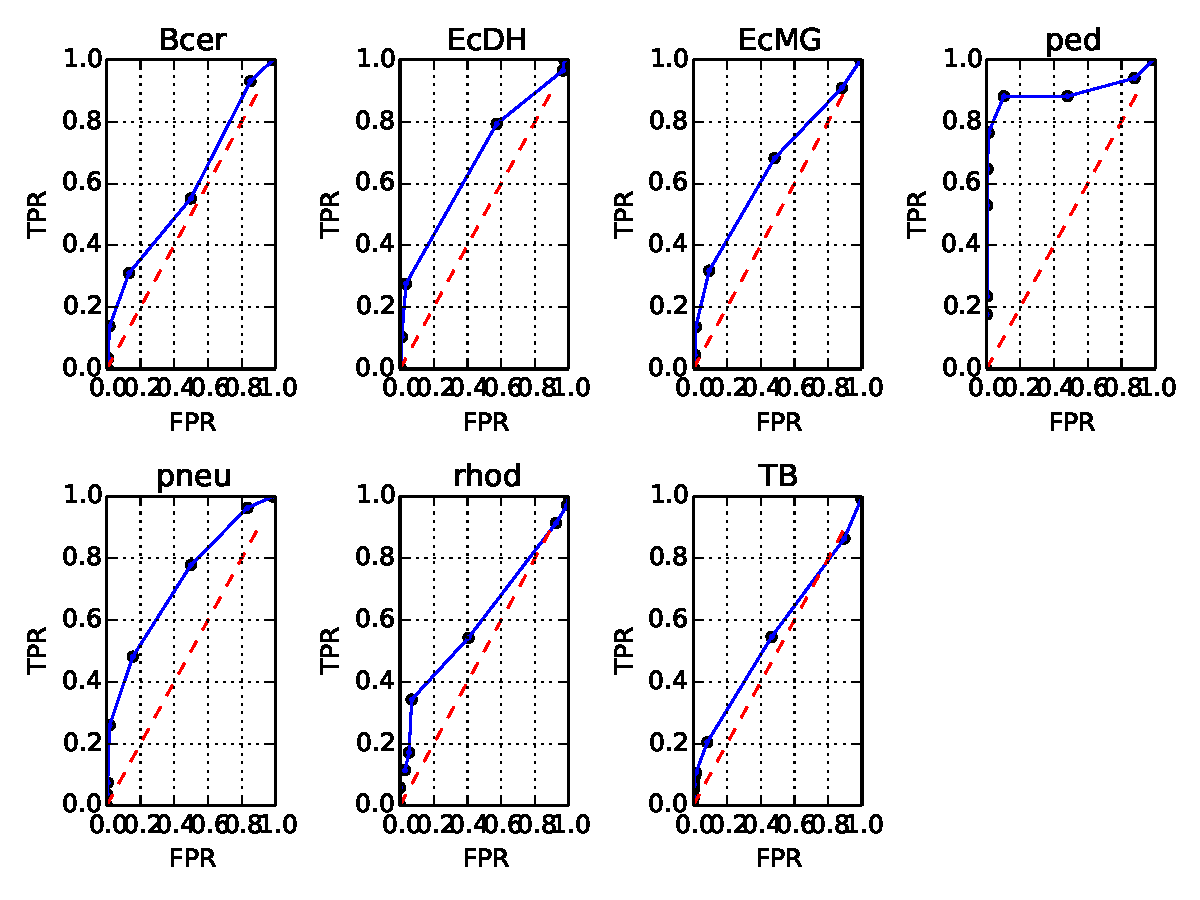
\includegraphics[width=0.8\textwidth]{illumina/allROC.pdf}}
\caption{ROC plots for the seven genomes containing misassemblies.\label{fig:ROCs}}
\end{figure}

\paragraph{Profiling}
Performance analysis was performed on a single core with 8 GB RAM available. Runtime analysis was performed using the python cProfile module. The memoryprofiler python module was used to analyse memory usage.

\subsection{Workflow Pipeline}
\textit{De novo} assemblies were prepared using the SPAdes Assembler, version 3.1.1~\cite{Bankevich2012}:

\texttt{spades.py -k 21,33,55,77 -t 4 \\ --hqmp1-12 bacteria.fastq.gz  --hqmp1-fr -o assembly}

The initial assembly quality was evaluated using QUAST~\cite{Gurevich2013} (version 2.3) to align the \textit{de novo} assembly to a reference genome:

\texttt{python quast.py -o results\_sample -t 16 \\  -R ref/reference.fna sample\_new.fasta }

  Following assembly, the same reads used to generate the assembly were aligned back to the \textit{de novo} assembly using BWA-MEM~\cite{li2013} (BWA version 0.7.10). A sorted BAM file of the resulting alignment was then prepared using SAMtools (version 1.1)~\cite{li2009}: 

\texttt{bwa index sample/scaffolds.fasta}

\texttt{bwa mem sample/scaffolds.fasta -p bacteria.fastq.gz | samtools view -bS - |  samtools sort - sample}

\texttt{samtools index sample.bam}

We identified misassemblies using NxRepair (version 0.13) as follows:

\texttt{python nxrepair.py sample.bam   sample/scaffolds.fasta sample\_scores.csv  sample\_new.fasta -img\_name sample\_new}


The default parameters used and their meanings are shown in Table~\ref{tab:parameters}. These have been optimised for Illumina Nextera mate pair libraries with a mean insert size of approximately 4 kb. For mate pair libraries with a much larger (smaller) insert size, the maxinsert and trim parameters may need to be increased (decreased).

\begin{table}
\begin{center}
\caption{NxRepair Parameters \label{tab:parameters}}
\begin{tabular}{llp{8cm}}
    \hline
    Parameter & Default Value & Meaning \\ \hline
    imgname & None & Prefix under which to save plots. \\
    maxinsert & 30000 &  Maximum insert size, below which a read pair is included in calculating population statistics.\\
    minmapq & 40 & Minimum MapQ value, above which a read pair is included in calculating population statistics.\\
    minsize & 10000 & Minimum contig size to analyse.\\ 
    prior & 0.01 & Prior probability that the insert size is anomalous.\\
    stepsize & 1000 & Step-size in bases to traverse contigs.\\
    trim & 4000 & Number of bases to trim from each side of an identified misassembly.\\
    T & -4.0 & Threshold in Z score (number of standard deviations from the mean) below which a misassembly is called.\\
    window & 200 & Window size across which bridging mate pairs are evaluated.\\ \hline
\end{tabular}
\end{center}
\end{table}

Finally we used QUAST~\cite{Gurevich2013} to evaluate the assembly quality following NxRepair by aligning the \textit{de novo} assembly to a reference genome as described above.


\section{Results}
We used NxRepair to correct \textit{de novo} assemblies from Replicate 2 of each of the nine bacterial genomes described above. Mate pair reads were trimmed, assembled using the SPAdes assembler (version 3.1.1)~\cite{Bankevich2012} and then aligned back to the assembled scaffold using BWA-MEM~\cite{li2013}. We used QUAST~\cite{Gurevich2013} to evaluate the assembly quality before and after NxRepair correction by aligning to an appropriate reference genome. For all NxRepair analyses, the default parameters, shown in Table~\ref{tab:parameters} were used. Fig.~\ref{fig:NxRepair} (A) shows a misassembled genome that contained several scaffolding errors identified by NxRepair (Fig.~\ref{fig:NxRepair} (B)). Following NxRepair correction, the most significant structural misassemblies were resolved (Fig.~\ref{fig:NxRepair} (C)). The improvement following NxRepair correction is shown for all nine genomes in Table~\ref{tab:improvement} (middle column). For two assemblies, errors were removed without reducing NGA50; for one genome, errors were removed but NGA50 was slightly reduced; for six genomes, three of which contained no large errors, no errors were found and the assembly was unchanged. We are not able to correct all misassemblies, as not all misassemblies exhibit a change in Z-score large enough to identify an error against the background score fluctuation caused by the wide insert size distribution of the Nextera mate pairs. 

To benchmark NxRepair's performance, we also attempted to identify assembly errors using the A5qc error correction module of the A5 Assembly pipeline~\cite{tritt2012}. The results are shown in Table~\ref{tab:improvement} (right hand column). For eight of the nine genomes evaluated, A5qc was unable to detect any errors. For the final genome (K. pneumoniae), A5qc did detect errors, but the contig-breaking process left Quast unable to align the resultant assembly to the reference genome. Re-scaffolding using the A5 scaffolder did allow reference alignment, but the assembly contained more misassemblies (15) than the original assembly. Consequently, we are confident that, for these high-quality alignments, NxRepair is a superior error-detection tool. 

Despite this good performance, it is clear that NxRepair is not able to find all misassemblies present. There are several reasons for this. Firstly, NxRepair's resolution is limited to relatively large-scale errors, as a very large disruption in mate pair insert sizes over a region of approximately 1 kb to significantly reduce the Z-score. Consequently, indel errors with a displacement smaller than 1 kb will not be detected. Secondly, NxRepair is limited by the intrinsic error rate of the mate pair library used. If the insert size distribution has a very wide variance, large fluctuations caused by assembly errors will be masked, making error correction more challenging. 

A number of improvements to NxRepair might mitigate these issues. Firstly, NxRepair currently identifies errors using a simple threshold applied to the total assembly support from spanning mate pairs, $D$. A more rigorous approach would implement a fully probabilistic method of error detection, using the distribution of spanning mate pair insert sizes to evaluate the relative probability of an error. 

Furthermore, NxRepair currently uses a user-defined prior probability of incorrect pairing and uses some simplistic thresholding to determine the parameters of the global insert size distribution. It would be possible to implement simultaneous co-estimatation of the mate pair error rate and the insert size distribution. In addition to relieving the user of estimating the error rate of their mate pair library, this would improve the accuracy of parameter estimation for the correct mate pairs, particularly for libraries with a large mate pair error rate. However, this would not necessarily translate into improved accuracy of error detection, as noise from the mate pair library would still mask true errors.        

\begin{table}[]
\begin{center}
\caption{Number of large misassemblies and NGA50 as reported by QUAST before (left) and after correction by NxRepair (middle) and A5qc (right). \label{tab:improvement}}
\resizebox{\textwidth}{!}{
{\begin{tabular}{llllllll}\hline
 & & \multicolumn{2}{l}{Before NxRepair} & \multicolumn{2}{l}{{\bf After NxRepair}} & \multicolumn{2}{l}{After A5qc} \\\hline
Genome & Genome size & No. & NGA50 & No. & NGA50 & No. & NGA50 \\\hline
B. cereus ATCC 10987 & 5,432,652 & 0 & 1,157,846 & 0 & 1,157,846 & 0 & 1,157,846 \\
E. coli K-12 substr. DH10B & 4,686,137 & 7 & 573,003 & 6 & 573,003 & 7 & 573,003 \\
E. coli K-12 substr. MG1655 & 4,641,652  & 3 & 693,692 & 3 & 693,692 & 3 & 693,692\\
L. monocytogenes EGDe & 2,944,528 & 0 & 1,496,613 & 0 & 1,496,613 & 0 & 1,496,613 \\
M. ruber DSM 2366 & 4,839,203 & 0 & 2,702,549 & 0 & 2,702,549 & 0 & 2,702,549 \\
P. heparinus DSM 2366 & 5,167,383 & 1 & 1,269,147 & 0 & 952,558 & 1 & 1,269,147 \\
K. pneumoniae MGH 78578 & 5,694,894 & 8 & 578,813 & 8 & 578,813 & - & - \\
R. sphaeroides 2.4.1 & 4,602,977 & 8 & 2,715,434 & 8 & 2,715,434 & 8 & 2,715,434 \\
M. tuberculosis H37Ra & 4,411,532 & 63 & 186,136 & 57 & 186,136 & 63 & 186,136 \\\hline
\end{tabular}}{}
}
\end{center}
\end{table}  


\subsection{Performance}
We evaluated the runtime and peak memory usage of NxRepair on each of the nine genomes analysed. The results are shown in Table~\ref{tab:performance}. The most memory and computationally intensive part of the NxRepair analysis is construction of the interval trees. The size of each interval tree is dependent on the contig size. Consequently, we expect both runtime and memory usage to scale with the size of the largest contig. 

\begin{table}
\begin{center}
\caption{NxRepair performance analysis. \label{tab:performance}}
\begin{tabular}{lll}
    \hline
    Bacterium & Total Time (s) & Memory Usage (MiB) \\ \hline
    B. cereus ATCC 10987 & 78 & 271 \\
    E. coli K-12 substr. DH10B & 123 & 444 \\
    E. coli K-12 substr. MG1655 & 70 & 260 \\
    L. monocytogenes EGDe & 97 & 383 \\
    M. ruber DSM 2366 & 259 & 565 \\
    P. heparinus DSM 2366 & 123 & 417 \\
    K. pneumoniae MGH 78578 & 59 & 227 \\
    R. sphaeroides 2.4.1 & 190 & 463 \\
    M. tuberculosis H37RaTB & 155 & 411 \\ 
    \hline
\end{tabular}
\end{center}
\end{table}

\begin{table}[h]
  \centering
  \caption{Summary of bacteria analysed and the relevant NCBI information on their reference genomes. There were two repeats of each strain. All 18 samples were prepared with the Nextera mate pair protocol and sequenced in a single MiSeq run using $2 \times 151$ bp reads. The untrimmed reads we used as input to NxTrim (3.9Gbp in all) are available from BaseSpace via \url{https://basespace.illumina.com/s/TXv32Ve6wTl9}.\label{data-description}}
\resizebox{\textwidth}{!}{
  \begin{tabular}{ll}
    \hline
    \textbf{Abbreviation:}             &    Bcer \\
    \textbf{Bacteria:}                 &    \emph{Bacillus cereus ATCC 10987} \\
    \textbf{Accession ID:}  &  NC\_003909, NC\_005707 \\ 
    \textbf{NCBI FTP:}                 &    \url{ftp.ncbi.nih.gov/genomes/Bacteria/Bacillus\_cereus\_ATCC\_10987\_uid57673/} \\
    \hline
    \textbf{Abbreviation:}             &    EcDH \\ 
    \textbf{Bacteria:}                 &    \emph{Escherichia coli str. K-12 substr. DH10B}\\ 
    \textbf{Accession ID:}              &    NC\_010473 \\ 
    \textbf{NCBI FTP:}     &    \url{ftp.ncbi.nih.gov/genomes/Bacteria/Escherichia\_coli\_K\_12\_substr\_\_DH10B\_uid58979/}\\
    \hline
    \textbf{Abbreviation:}             &   EcMG \\
    \textbf{Bacteria:}                 & \emph{Escherichia coli str. K-12 substr. MG1655}\\
    \textbf{Accession ID:}            & NC\_000913    \\ 
    \textbf{NCBI FTP:}       & \url{ftp.ncbi.nih.gov/genomes/Bacteria/Escherichia\_coli\_K\_12\_substr\_\_MG1655\_uid57779/}\\
    \hline
    \textbf{Abbreviation:}             &   list\\ 
    \textbf{Bacteria:}                 &\emph{Listeria monocytogenes}\\  
\textbf{Accession ID:}              & NC\_003210 \\ 
\textbf{NCBI FTP:}     & \url{ftp.ncbi.nih.gov/genomes/Bacteria/Listeria\_monocytogenes\_EGD\_e\_uid61583/}\\
\hline
\textbf{Abbreviation:}             &  meio \\ 
\textbf{Bacteria:}                 &\emph{Meiothermus ruber DSM 1279}\\ 
\textbf{Accession ID:}             &NC\_013946 \\ 
\textbf{NCBI FTP:}      & \url{ftp.ncbi.nih.gov/genomes/Bacteria/Meiothermus\_ruber\_DSM\_1279\_uid46661/}\\
   \hline
\textbf{Abbreviation:}             &  ped \\
\textbf{Bacteria:}                 &\emph{Pedobacter heparinus DSM 2366}\\
\textbf{Accession ID:}                 & NC\_013061 \\ 
\textbf{NCBI FTP:}  & \url{ftp.ncbi.nih.gov/genomes/Bacteria/Pedobacter\_heparinus\_DSM\_2366\_uid59111/}\\
   \hline
\textbf{Abbreviation:}             &   pneu \\
\textbf{Bacteria:}                 & \emph{Klebsiella pneumoniae subsp. pneumoniae MGH 78578}  \\
\textbf{Accession ID:}              & NC\_009648, NC\_009649, NC\_009650, NC\_009651, NC\_009652, NC\_009653 \\ 
\textbf{NCBI FTP:}     & \url{ftp.ncbi.nih.gov/genomes/Bacteria/Klebsiella\_pneumoniae\_MGH\_78578\_uid57619/}\\
   \hline
\textbf{Abbreviation:}             &  rhod \\ 
\textbf{Bacteria:}                 &\emph{Rhodobacter sphaeroides 2.4.1}\\ 
\textbf{Accession ID:}                 &NC\_007488, NC\_007489, NC\_007490, NC\_007493, NC\_007494, NC\_009007, NC\_009008\\ 
\textbf{NCBI FTP:}  & \url{ftp.ncbi.nih.gov/genomes/Bacteria/Rhodobacter\_sphaeroides\_2\_4\_1\_uid57653/}\\ 
   \hline
\textbf{Abbreviation:}             &  TB \\
\textbf{Bacteria:}                 & \emph{Mycobacterium tuberculosis H37Ra}\\ 
\textbf{Accession ID:}               &NC\_009525 \\ 
\textbf{NCBI FTP:}    & \url{ftp.ncbi.nih.gov/genomes/Bacteria/Mycobacterium\_tuberculosis\_H37Ra\_uid58853/}\\ 
   \hline
  \end{tabular}
}
\end{table}

\begin{table}[]
\begin{center}
{
\caption{Yield in bp, mean base quality and average read length after adapter removal, as well as the raw NGA50 score prior to NxRepair analysis for all genomes analysed.\label{tab:yield}}
{\begin{tabular}{lllll}\hline
Genome & Yield [bp] & Mean base quality & Mean read length & Raw NGA50 \\\hline
B. cereus lib1 & 140,034,231 & 30.83 & 120.50 &  1,157,404\\
B. cereus lib2 & 150,883,336 & 31.69 & 124.08  & 1,157,846\\
E. coli DH10B lib1 & 229,164,175 & 31.50 & 127.55 & 576,143\\
E. coli DH10B lib2 & 167,955,255 & 31.19 & 126.49 & 573,003\\
E. coli MG1655 lib1 & 138,893,204 & NaN & 104.56 & 640,732\\
E. coli MG1655 lib2 & 164,490,239 & 31.93 & 129.67 & 693,692\\
L. monocytogenes lib1 & 197,796,210 & 32.66 & 129.79 & 1,496,615\\
L. monocytogenes lib2 & 161,114,700 & 31.81 & 125.79 & 1,496,613\\
M. ruber lib1 & 180,542,545 & 29.96 & 123.69 & 3,095,733\\
M. ruber lib2 & 150,298,958 & 31.09 & 129.40 & 2,702,549\\
P. heparinus lib1 & 186,070,764 & 32.21 & 127.30 & 1,269,259\\
P. heparinus lib2 & 146,448,694 & 31.32 & 124.00 & 1,269,147\\
K. pneumoniae lib1 & 182,614,602 & 31.86 & 131.70 & 577,220\\
K. pneumoniae lib2 & 166,306,322 & 31.82 & 130.28 & 578,813\\
R. sphaeroides lib1 & 184,138,610 & 30.08 & 127.99 & 3,181,390\\
R. sphaeroides lib2 & 210,961,284 & 30.12 & 129.79 & 2,715,434\\
M. tuberculosis lib1 & 211,892,634 & 30.43 & 127.37 & 184,170\\
M. tuberculosis lib2 & 177,615,358 & 30.06 & 126.82 & 186,136\\\hline
\end{tabular}}{}
}
\end{center}
\end{table}  


\section{Conclusions}
NxRepair is a simple error correction module that can be used to rapidly identify and remove large scale errors from \textit{de novo} assemblies using Nextera mate pair reads. We evaluated NxRepair using \textit{de novo} assemblies of nine bacterial genomes prepared using the SPAdes assembler, showing that of the six genomes containing misassemblies, three could be improved by NxRepair correction; compared with no improvements made by the A5qc module. SPAdes is the current state of the art in bacterial genome assembly and explicitly uses mate pair information during both contig construction and scaffolding. Even in these excellent assemblies, NxRepair could identify misassemblies and improve the assembly quality. We predict that NxRepair will be even more useful for identifying errors in \textit{de novo} assemblies where mate pair information was used only at the scaffolding stage. 

NxRepair is freely available online. It can be downloaded from the Python Package Index (\url{https://pypi.python.org/pypi/nxrepair}) and run with a single call from the command line, making it an attractive option for fast evaluations of and improvements to assembly quality. The source code is available on GitHub (\url{https://github.com/rebeccaroisin/nxrepair}), facilitating easy incorporation into user assembly pipelines.  

\chapter{Conclusions and Future Work}
\label{chap:conclusions}

\section{General Conclusions}
This thesis presents three years' work on understanding and improving the analysis tools used in confocal smFRET experiments. This work has involved both implementing and benchmarking existing techniques, as well as implementing and thoroughly evaluating novel methodologies. It is hoped that this work provides a strong foundation for rigorous work by other researchers in this field.

\subsection{pyFRET}
Chapter~\ref{chap:pyfret} described the development and release of an open source software library for the analysis of confocal smFRET data. For researchers working in different research environments to be able to cross-compare their results effectively, it is necessary that they have an effective method to describe and share their analysis tools and to select the best analysis tools for their specific research problem. Furthermore, smFRET data is quite sensitive to the analysis methods used.  As shown, both the specific analysis tools used and the method of their usage can quite significantly influence the appearance of the processed data and hence the outcome of downstream analyses. Unfortunately, to date there has been no culture of publishing the code or smFRET data analysis tools, which has made it difficult for researchers to compare the effectiveness and efficiency of different analysis methods.

To overcome these challenges, pyFRET, a software library that implements many of the main methodologies for analysis of smFRET data, was developed and released. pyFRET is open source and fully documented. This provides both a toolkit of analysis methods that can be freely accessed by other researchers and a platform for researchers to contribute and benchmark novel analysis methods. A rigorous comparison of different data collection and analysis methods for confocal smFRET data was also described. The evaluation presented here identifies the clear superiority of alternating excitation schemes that provide direct access to acceptor excitation information, enabling thresholding-based event selection to be carried out without bias. It is show that without direct access to information about acceptor emission, the more complex APBS and DCBS burst search algorithms display biases comparable to those seen from the simple AND and SUM thresholding algorithms, despite significantly increased space requirements and computational complexity. It is hoped that this work will facilitate research by other scientists, who can now quickly and effectively select the correct analysis tool for their data, as well as providing a platform for the publication and benchmarking of novel analysis methods.

\subsection{Inference Analysis of smFRET Data}
Thresholding-based event selection for confocal smFRET data necessarily discards a significant fraction of the smFRET dataset, including not only noise but also a large fraction of fluorescence emission events. Furthermore, as shown in Chapter~\ref{chap:pyfret}, in the absence of direct information about acceptor emission behaviour, thresholding criteria are biased and do not select a random subset of fluorescent events, resulting in distortion of downstream analyses. To overcome these challenges, a novel analysis method was developed, based on model-based Bayesian inference, that can simultaneously co-infer the values of all parameters of interest in a confocal smFRET dataset.

Chapter~\ref{chap:inference} presents the development and evaluation of this novel tool. This evaluation shows that model-based inference is an effective tool for analysis of smFRET data and that the concentrations and intramolecular distances of single fluorescent populations or of a mixture of two fluorescent populations can be accurately inferred. The full source code for our inference analysis is freely available online. This work provides a strong foundation for the application of model-based inference to a wider range of smFRET datasets and demonstrates the proof of concept that model-based inference is both feasible and fruitful as a method of data analysis for this research field.  

\subsection{Inference Analysis of Oligomer Sizing}
Chapter~\ref{chap:sizing} extends the concept of model-based inference and applies this form of analysis to the problem of accurately sizing heterogeneous mixtures of fluorescently labelled oligomers. A significant research effort has been made in the Klenerman group to develop experimental methodologies to allow accurate characterisation of the oligomerization reactions observed in amyloidosis. The data analysis side of this effort has been somewhat neglected, allowing unfounded assumptions about the data collected to significantly reduce the accuracy of calculated oligomer size distributions.

The work presented in this chapter demonstrates, through a comparison of simulated datasets and data from simple, well-controlled experiments, that the heterogeneity observed in photon emission is not dominated, as would be hoped, by the number of fluorophores attached to a molecule. Instead, underlying photophysical processes, including, but not limited to, photobleaching, photoblinking, and the diffusion pathway of molecules through the confocal volume, have a more significant effect on the number of photons observed. Although this research was not able to provide a greatly improved analysis technique, it is hoped that the thorough evaluation presented here of the challenges encountered in attempting to accurately determine oligomer sizes, even in well-characterised, homogeneous samples, demonstrates the importance of thoroughly examining all assumptions implicit in any method of data analysis.   

\subsection{NxRepair}
The final results chapter, Chapter~\ref{chap:illumina}, presented work performed in a different research field; namely the development of NxRepair, an error correction tool for \emph{de novo} assemblies of bacterial genomes assembled from Illumina's Nextera mate pair reads. Although long-read technologies are being developed, these are either still experimental or prohibitively expensive for normal use. Consequently, the challenge of accurately reconstructing the sequence of an entire genome from short read sequences remains current. 

The work presented in this chapter demonstrates a novel method for error identification and error correction based on probabilistic analysis of the insert size distribution when mate pair reads are aligned back to the \emph{de novo} assembly. NxRepair is available online for free download and the source code is hosted on the popular code repository GitHub.  This chapter presents a comprehensive evaluation of the performance of NxRepair using multiple bacterial genomes, demonstrating its superior performance when compared to the most popular existing error correction tool.

\section{Applications and Future Work}
The work presented in this thesis, and summarized above, provides a stable foundation for further work to consolidate and improve the analysis of smFRET data. Some of the results presented have encouraged experimental method development to allow more rigorous analysis of smFRET data. To conclude this thesis, some of the applications and extensions that are being considered as a result of the work described here are now summarized. 

\subsection{Open Source Software for smFRET}
pyFRET, the open source library of data analysis tools for smFRET currently provides sufficient functionality for a researcher to perform a full analysis of smFRET data collected from a range of different experiment types using a number of different methods. As the source code that implements the analysis tools, as well as the tools themselves, is freely available online it is straightforward for researchers to understand how the analysis works and to modify the tools as they require. This prevents new users of smFRET technology from needing to develop their analysis tools from scratch in order to be able to analyse their data. 

Furthermore, as experimental technologies develop and improve, it is to be expected that new analysis tools will also be required. pyFRET provides a central repository to the community to which new techniques can be added, to allow easy access and evaluations; and against which new techniques can be benchmarked; enabling researchers to make fully informed descisions about which analysis tools and experiemental methodologies to use in their research.

pyFRET already has users outside of the Klenerman research group and requests for additional features have been satisfied. There is clearly considerable work to do to allow pyFRET to become useful to a wider swathe of the smFRET research community. However, it is hoped that its existence encourages a more open, collaborative approach to smFRET data analysis and method development. 

\subsection{Inference Analysis of smFRET Data}
The work on inference analysis on smFRET data presented here clearly shows the feasibility of inference analysis as a method of analysing smFRET data. It also highlights considerable extensions and improvements to the inference method as presented here, the implementation of which would considerably increase the utility of inference as an analysis tool. The two most important of these are:

\begin{enumerate}
\item The implementation of reversible jump Monte Carlo inference~\cite{green1995}.
\item The release of the inference analysis as a software package.
\end{enumerate}

In its current implementation, the inference analysis cannot infer the number of fluorescent populations in a mixture; the number of populations must be given. This is a considerable limitation, as the number of fluorescent populations is frequently unknown. At present, determining the number of fluorescent populations can only be carried out by performing inference multiple times, modifying the number of expected fluorescent populations, and then manually inspecting the results obtained. Implementation of reversible jump Monte Carlo sampling would make this model selection step part of the inference analysis and would greatly increase the attraction of inference as a method of smFRET data analysis. 

Similarly, although the source code for the inference analysis can be viewed and downloaded from an open source code repository, the code is not packaged or documented in a manner that makes it easy to use. Packaging the analysis code as a software package, for example by incorporating it into the pyFRET framework, would make this analysis tool more accessible to other researchers. Making both of these improvements is likely to significantly improve the reception of inference analysis by smFRET researchers.

\subsection{Accurate Sizing of Fluorescent Oligomers}
Although the work on accurate oligomer sizing using inference methods was the least successful piece of research presented in this thesis in terms of successful method development, it is the work that has presented the greatest number of opportunities for further work. The results that are presented here conclusively demonstrate the role of both photophysics and the underlying experimental methodology in preventing accurate assessment of oligomer size distributions based on fluorescence data. These conclusions have led to significant re-evaluation of the experimental methods used and to the proposal of several modifications to the research methodology that may enable a more quantitative evaluation of oligomer sizes.

Specifically, the Klenerman group is currently constructing a novel confocal microscope that uses acousto-optic modulation to allow uniform excitation of the confocal volume in the $x$-dimension. By flowing labelled molecules rapidly across this region of uniform excitation using nanofluidic channels that confine the molecules to a narrow region in the $y$-dimension, it may be possible to reduce the experimental sources of emission heterogeneity. Similarly, fluorophore performance is currently being evaluated, to find commercially available structures that are more robust to photobleaching and photoblinking behaviour. A thorough evaluation of the new experimental set-up is currently in progress and it is hoped that this may lead to a more quantitative experimental methodology for determining sizes and size distributions.

\subsection{Error Detection in \emph{de novo} Assemblies}
The work presented on error correction in \emph{de novo} assemblies is predominantly self contained. An open-source error correction tool was developed and released. This tool is currently used by bioinformaticians at Illumina; an evaluation of the tool's performance forms the basis for a peer reviewed publication~\cite{murphy2015}. Extensions of this tool include modifications to enable larger genome assemblies to be evaluated and to allow evaluation of \emph{de novo} assemblies prepared using alternative sequencing methodologies, such as the long-reads from Nanopore sequencing that can be ``threaded'' through a de Bruijn graph to resolve ambiguities~\cite{Koren2015}. Modification of the tool to enable chaining with other assembly and quality control tools is also possible. Implementation of these additions depends on demand and uptake from other bioinformaticians. It is hoped that NxRepair finds an interested user-base within the bioinformatics research community.


%\nocite{*}

\bibliographystyle{unsrt}
\bibliography{thesis}


\end{document}